\section{Optimization of number of iterations for unfolding}
% This section examines the effect of conducting the stress test with a migration matrix filled from \pow+\py\ \ttbar+the nominal 3\% Wt. One thousand pseudoexperiments are taken from Poisson variations of the number of jets in each bin. Correction factors for event selection and \pt\ matching are taken from \powpy. The number of iterations is varies from 2 to 10.
\label{app:stressiter}


The optimization of the number of iterations for the Bayesian unfolding is done by studying the performance of the unfolding in stress tests. The response matrix is taken from the baseline ttbar sample(\powpy\ + 3\% $Wt$). The input reconstructed distribution are obtained from each of NLO alternate ttbar generators discussed in Chapter~\ref{ss:mcsignal}. The same 3\% $Wt$ contribution is included for each generator.

One thousand pseudoexperiments are constructed from each generator as in Chapter~\ref{ss:stress}. These pseudoexperiments are then unfolded, varying the number of iterations from one to nine. A number of metrics are studied to understand the behavior of the unfolding.
\begin{description}
\item[Mean bias:] The bias is calculated as $N_{\textrm{ unfolded}}-N_{\textrm{ true}}$ averaged one thousand pseudoexperiments.

Figures \ref{fig:powhwbias}-\ref{fig:mcnlohwbias} show the mean and $\sigma$ of the bias for each of the 41 bins, obtained from a Gaussian fit over all one thousand pseudoexperiments for one through four iterations. Figures \ref{fig:powhwfrbias}-\ref{fig:mcnlohwfrbias} show the fractional bias, taken as the ratio of the bias spectrum to the truth. As the number of iterations is increased, the $\sigma$ of the bias increases. 

To understand whether the mean of the bias improves with the number of iterations, the bias averaged over all 41 bins is calculated in Table~\ref{t:bias} for $N_{\textrm{ iter}}$ 1-9. Bin-by-bin unfolding is also included for comparison. Bin-by-bin unfolding produces an mean bias of $\sim$300 jets. For Bayesian unfolding, the bias varies from $<$1 up to $\sim$6 jets depending on generator. This represents a fractional bias of 0.3-2\% of the total number of jets.In all cases, the bias depends only weakly on $N_{\textrm{ iter}}$, but tends to increase with increasing $N_{\textrm{iter}}$.
\item[Mean bias$^2$:]The bias squared is calculated as
$$
\frac{1}{N_{\textrm{bins}}} \sum_{j=1}^{N_{\textrm{bins}}} \left (\frac{1}{N_{\textrm{pseudo}}} \sum_{i=1}^{N_{\textrm{pseudo}}} N^i_{\textrm{ unfolded}}-N^{i}_{\textrm{ true}} \right )_{j}^{2}
$$
Table~\ref{t:biassq} provides the mean bias$^{2}$ for bin-by-bin unfolding and Bayesian unfolding with $N_{\textrm{iter}}$=1-9. The bin-by-bin unfolding has a mean bias$^2$ of $\sim 10\e{6}$ jet$^2$. Depending on the generator, the mean bias$^2$ for one iteration varies from $\sim$20 to $\sim$80 jets$^2$.  In all cases, the bias$^2$ increases with $N_{\textrm{ iter}}$. For most generators, the mean bias$^2$ roughly stabilizes for $N_{\textrm{ iter}} > 4$. 
\item[Mean \textrm{ret}urned error:] The mean \textrm{ ret}urned error is defined as

$$
\frac{1}{N_{\textrm{bins}}} \sum_{j=1}^{N_{\textrm{bins}}} \frac{1}{N_{\textrm{pseudo}}} \sum_{i=1}^{N_{\textrm{pseudo}}} {\sigma_{\textrm{ ret}}}^{i}_{j}
$$  

where ${\sigma_{\textrm{ ret}}}^{i}_{j}$ is the uncertainty by \texttt{RooUnfold} for bin $j$ and pseudoexperiment $i$. These mean \textrm{ ret}urned errors are shown in Table~\ref{t:err} for Bayesian unfolding with $N_{\textrm{ iter}}$=1-9. For one iteration, the mean error is $\sim$ 8 jets for all generators. In all cases, the error increases with $N_{\textrm{ iter}}$.
\item[Pull:] The pull is calculated as $(N_{\textrm{ unfolded}}-N_{\textrm{ true}})/\sigma$, where $\sigma$ is the bin error \textrm{ ret}urned by \texttt{RooUnfold}.
Figures~\ref{fig:powhwpull}-\ref{fig:mcnlopull} show the mean and $\sigma$ of the pull for each of the 41 bins, obtained from a Gaussian fit over all One thousand pseudoexperiments for one through four iterations. The scatter in the means of the pull shows the same behavior as that of the bias. For $N_{\textrm{ iter}}$=1, the \textrm{ ret}urned error does not properly represent the spread seen among the pseudoexperiments. For $N_{\textrm{ iter}} \geq 2$, the width of the pull is close to 1 for all generators and all bins.  
\item[\chisq:] All of the metrics listed are insensitive to bin-to-bin correlations. To understand whether the unfolding is properly handling such correlations, the unfolded and fully corrected distributions for each generator are compared to that generator's truth distribution using the full chisq calculation in Equation\ref{eq:unfchi2}. Table~\ref{t:stresschi} and Figure~\ref{f:stresschi} show the \chisq\ for varying number of iterations.

For the baseline generator, the chisq is properly normalized, giving $\sim$43 for 41 degrees of freedom, independent of $N_{\textrm{ iter}}$. For the alternative generators, with $N_{\textrm{ iter}}=1$, the chisq vary from $\sim$140-$\sim$260. As $N_{\textrm{ iter}}$ increases, the chisq decreases, roughly stabilizing for $N_{\textrm{ iter}} \geq 6$. This decrease in chisq is largely due to the increase in size of the uncertainty rather than improvement in the unfolding itself, as seen from the above metrics. 
\end{description}
The metrics above do not point to a single optimal choice of $N_{\textrm{ iter}}$. The bias and the bias$^{2}$ increase slowly with $N_{\textrm{ iter}}$. The error uniformly increases with increasing $N_{\textrm{ iter}}$. The pulls indicate that for $N_{\textrm{ iter}}=1$, the unfolding does not \textrm{ ret}urn properly normalized uncertainties. The chisq metric favors a $N_{\textrm{ iter}}=4-6$. Because $N_{\textrm{ iter}}=2$ provides properly normalized uncertainties (as shown by the pull) and small values for the bias and bias$^2$, this is chosen as the optimal number of iterations. Because the chisq \textrm{ ret}urned for alternate generators is not properly normalized, a systematic uncertainty must be assigned. The procedure for assigning this uncertainty is described in Section~\ref{ss:unfsystt}. 


%\section{Bias \mcnlohw}

%\section{Bias \pow+\hw}
\begin{figure}
\begin{subfigure}[]{0.5\textwidth}
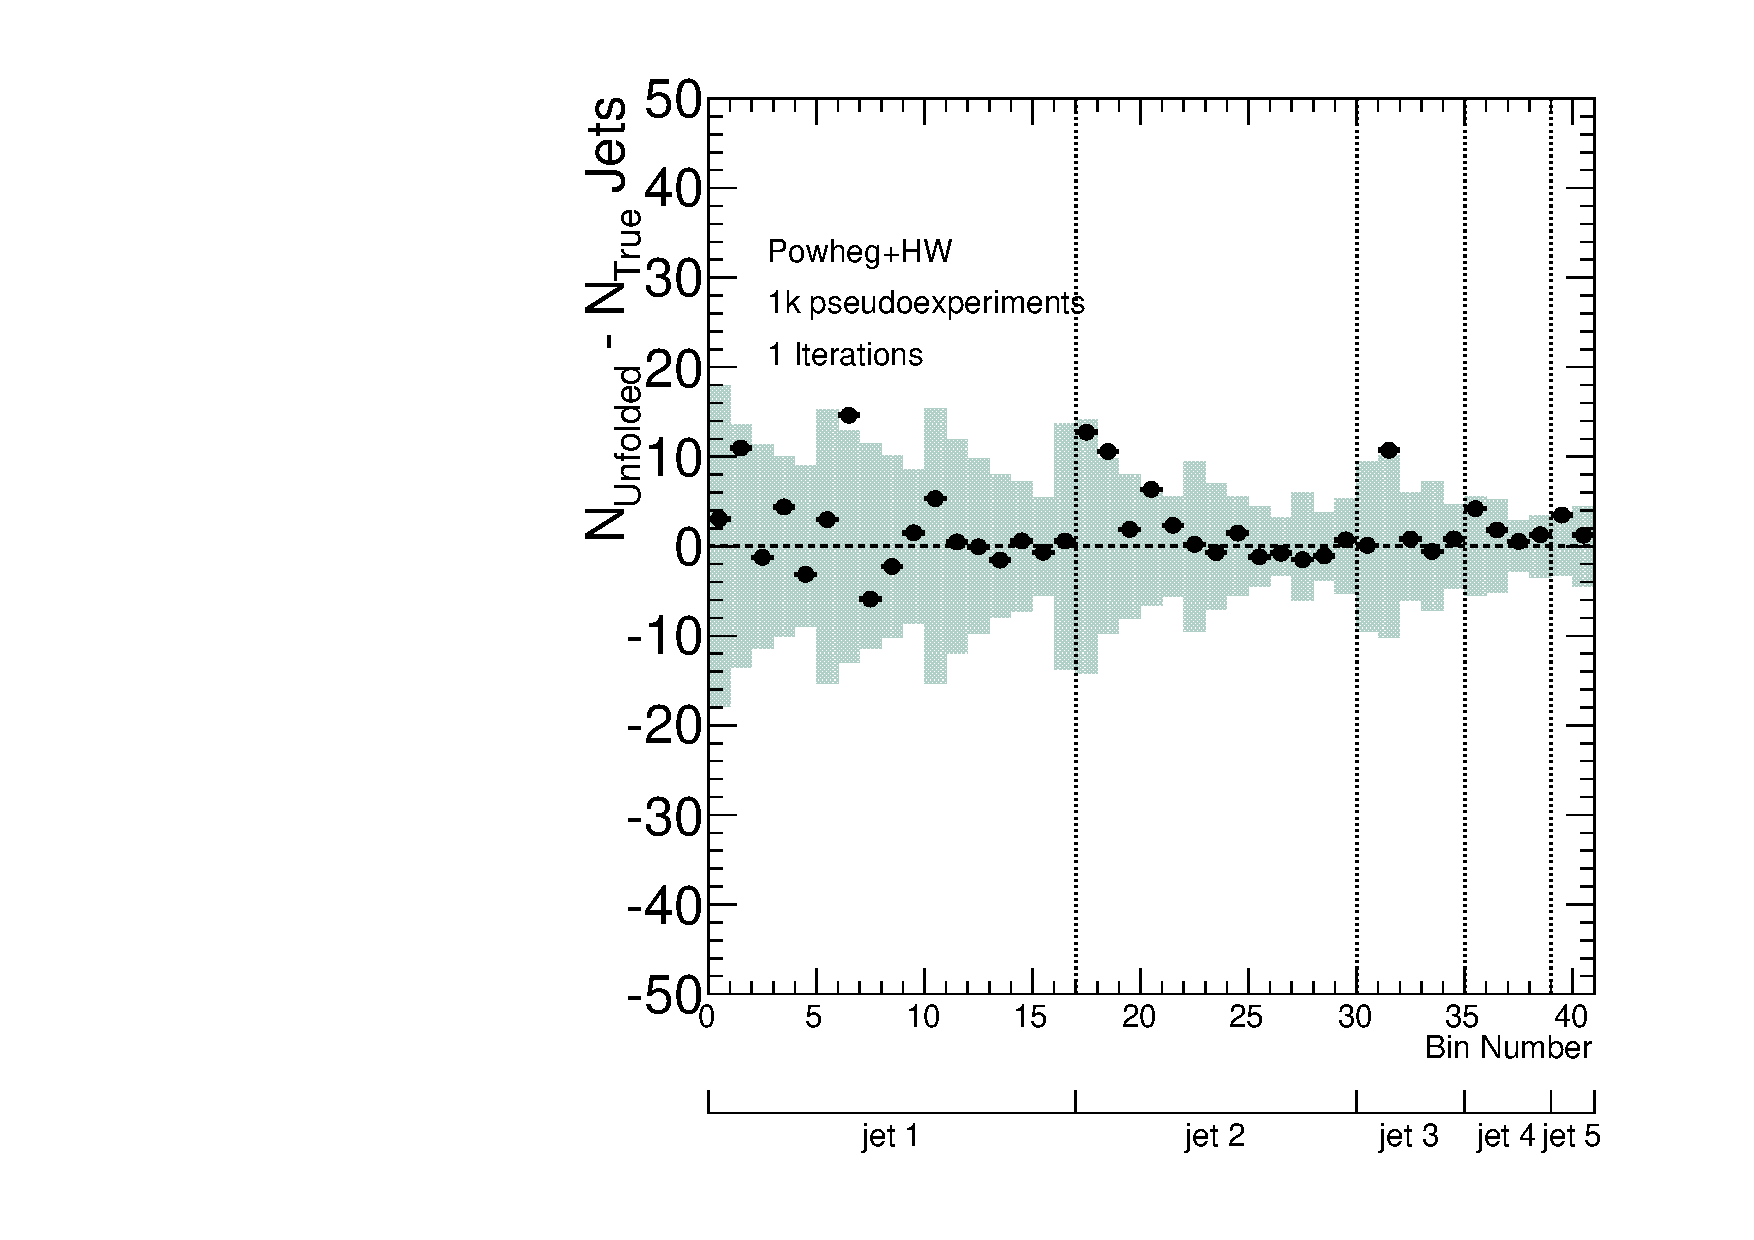
\includegraphics[width=\textwidth]{fig/Stress/105860atlfast/Bias1Iterations.pdf}
\end{subfigure}
~
\begin{subfigure}[]{0.5\textwidth}
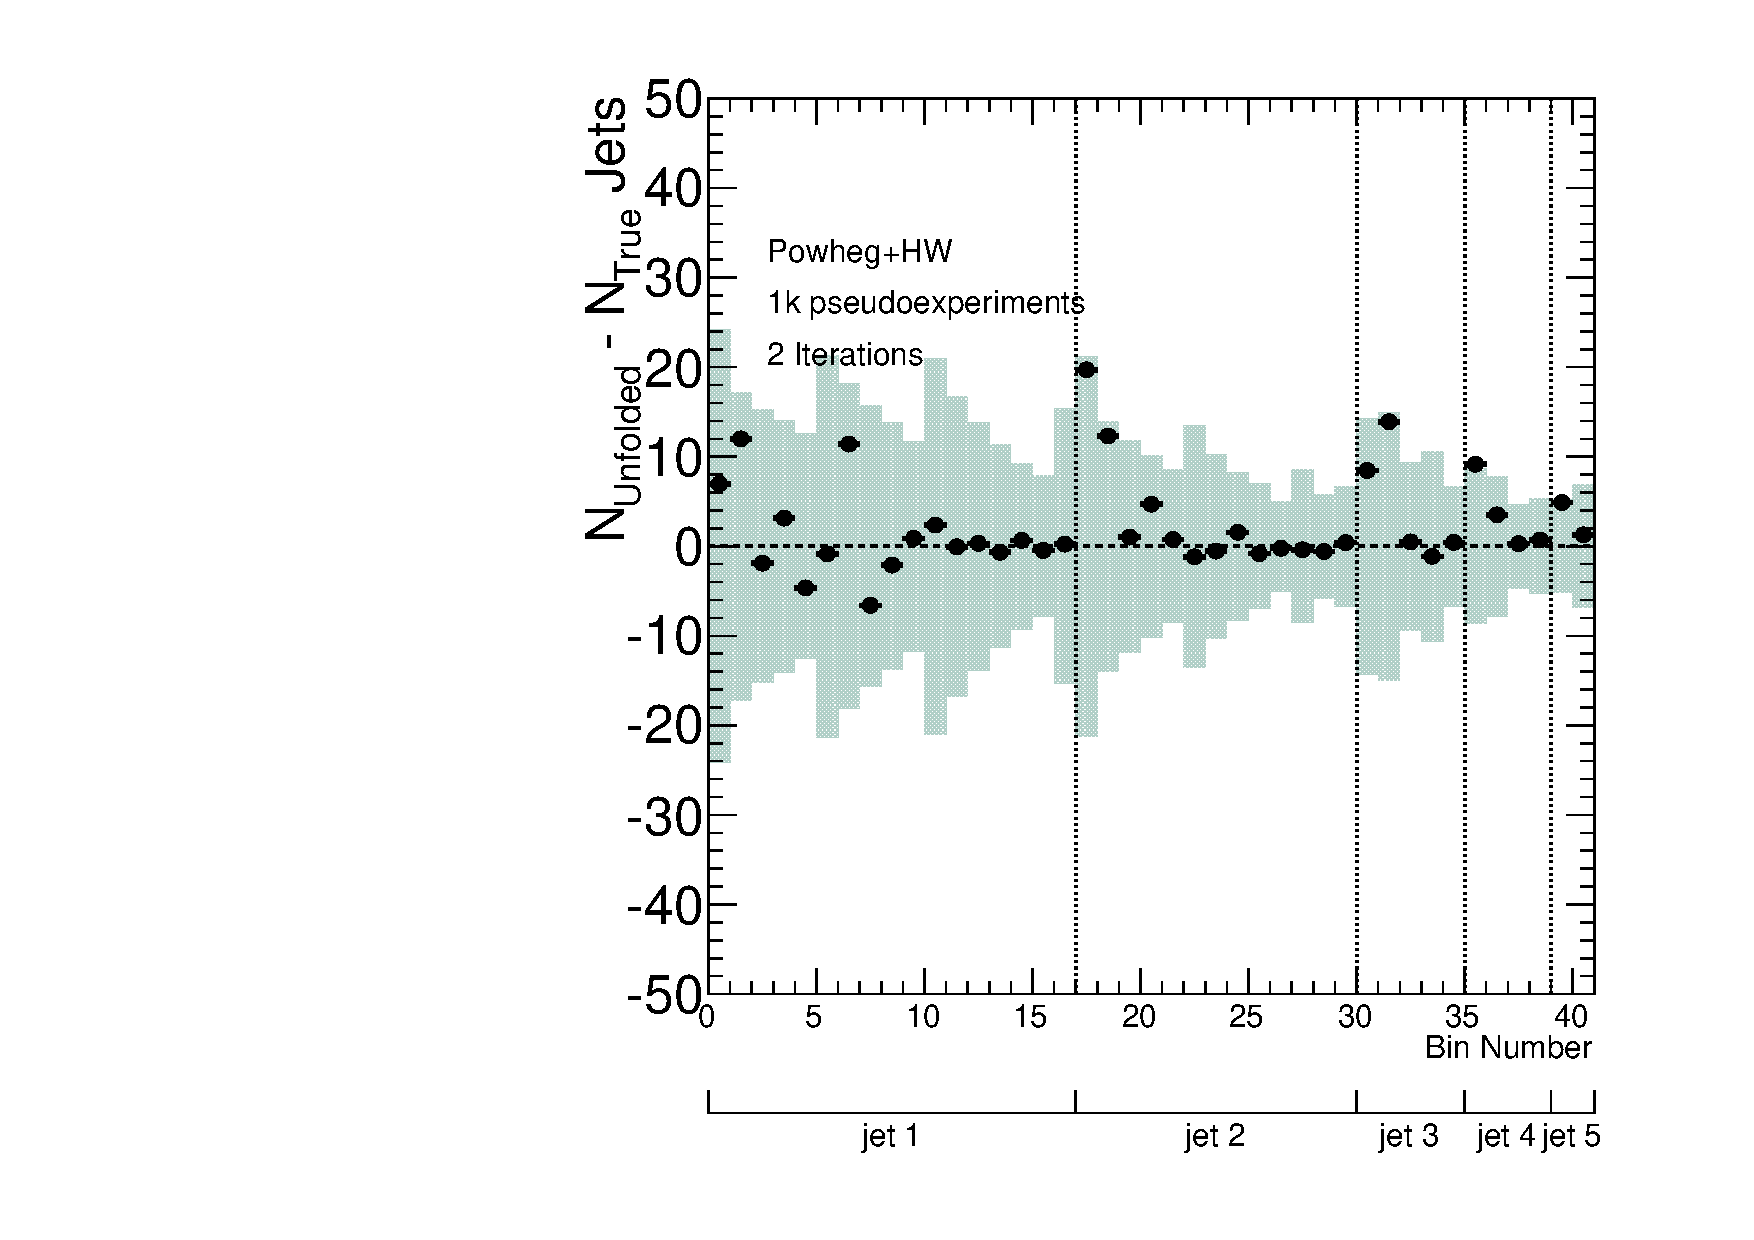
\includegraphics[width=\textwidth]{fig/Stress/105860atlfast/Bias2Iterations.pdf}
\end{subfigure}
\\
\begin{subfigure}[]{0.5\textwidth}
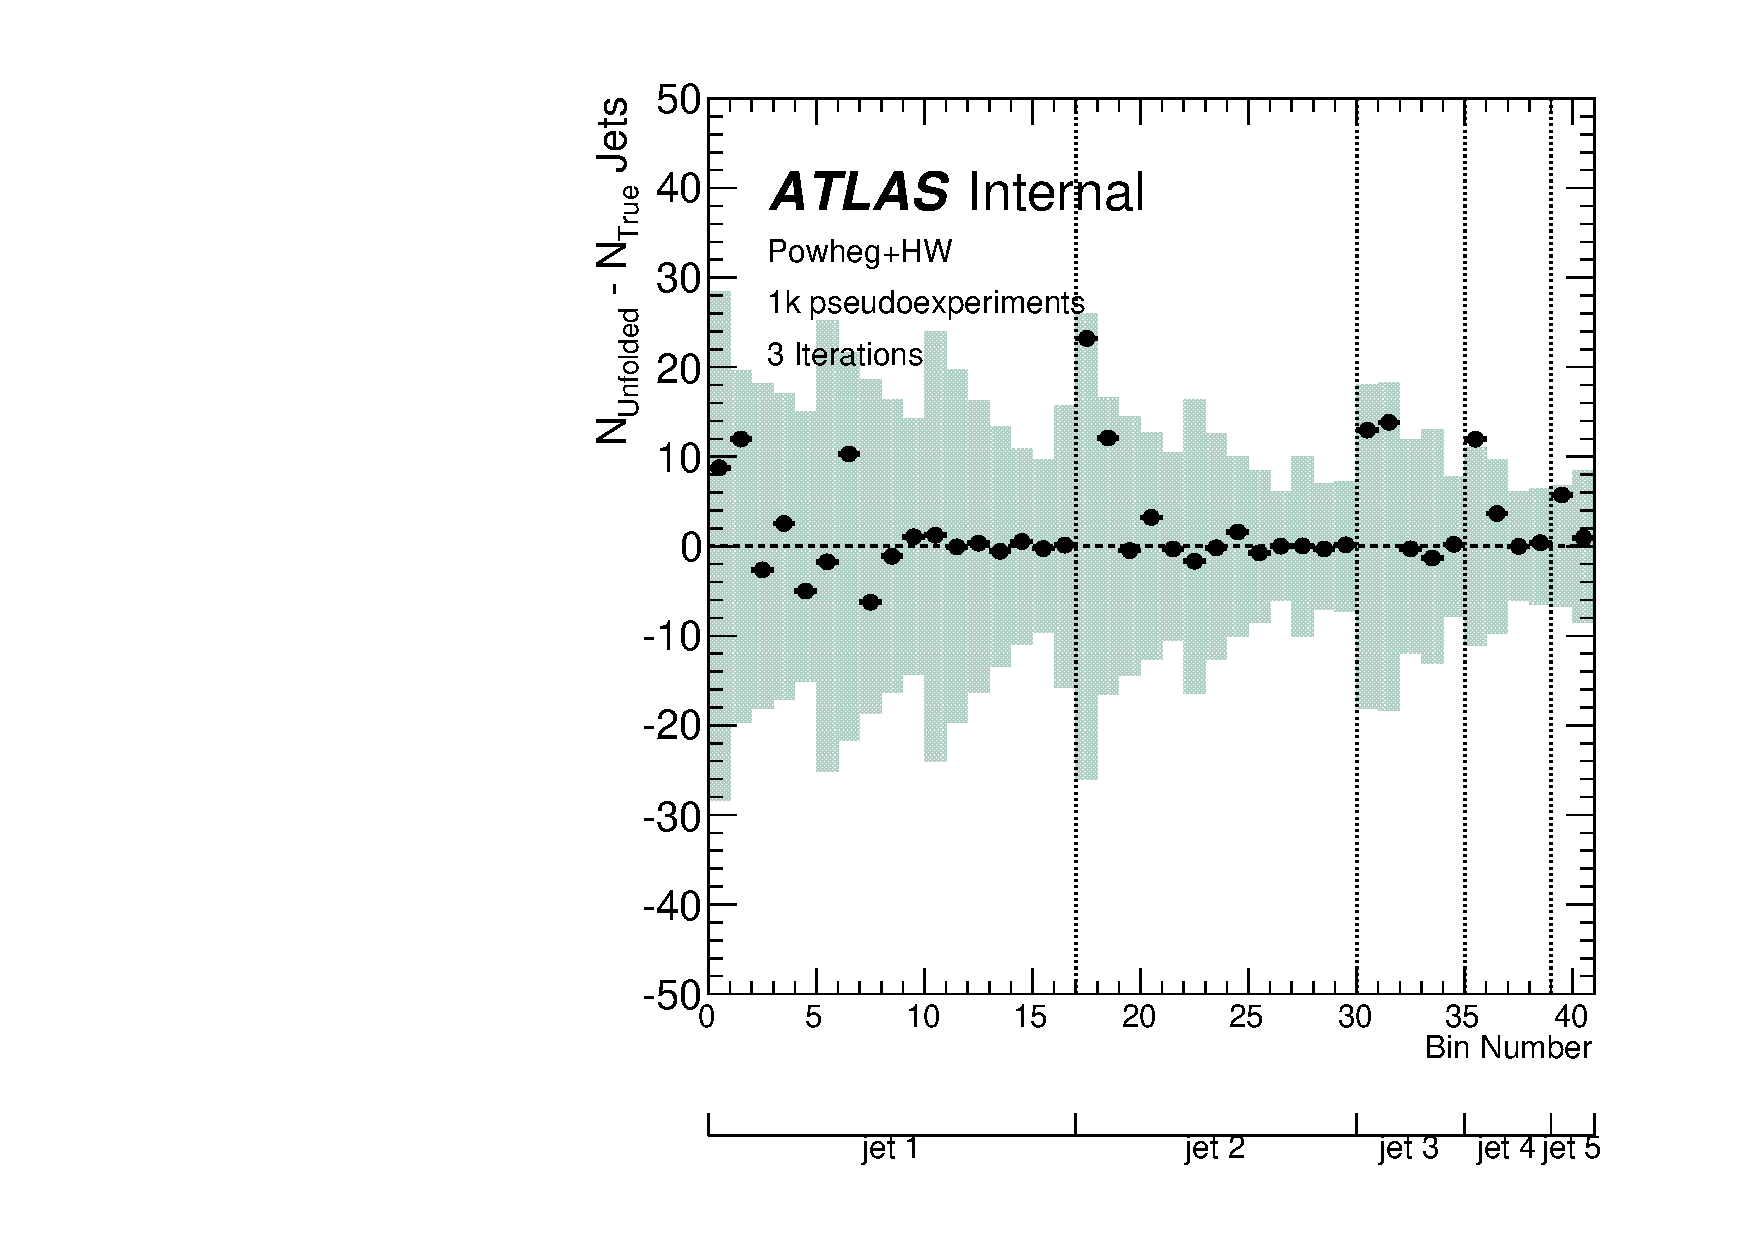
\includegraphics[width=\textwidth]{fig/Stress/105860atlfast/Bias3Iterations.pdf}
\end{subfigure}
~
\begin{subfigure}[]{0.5\textwidth}
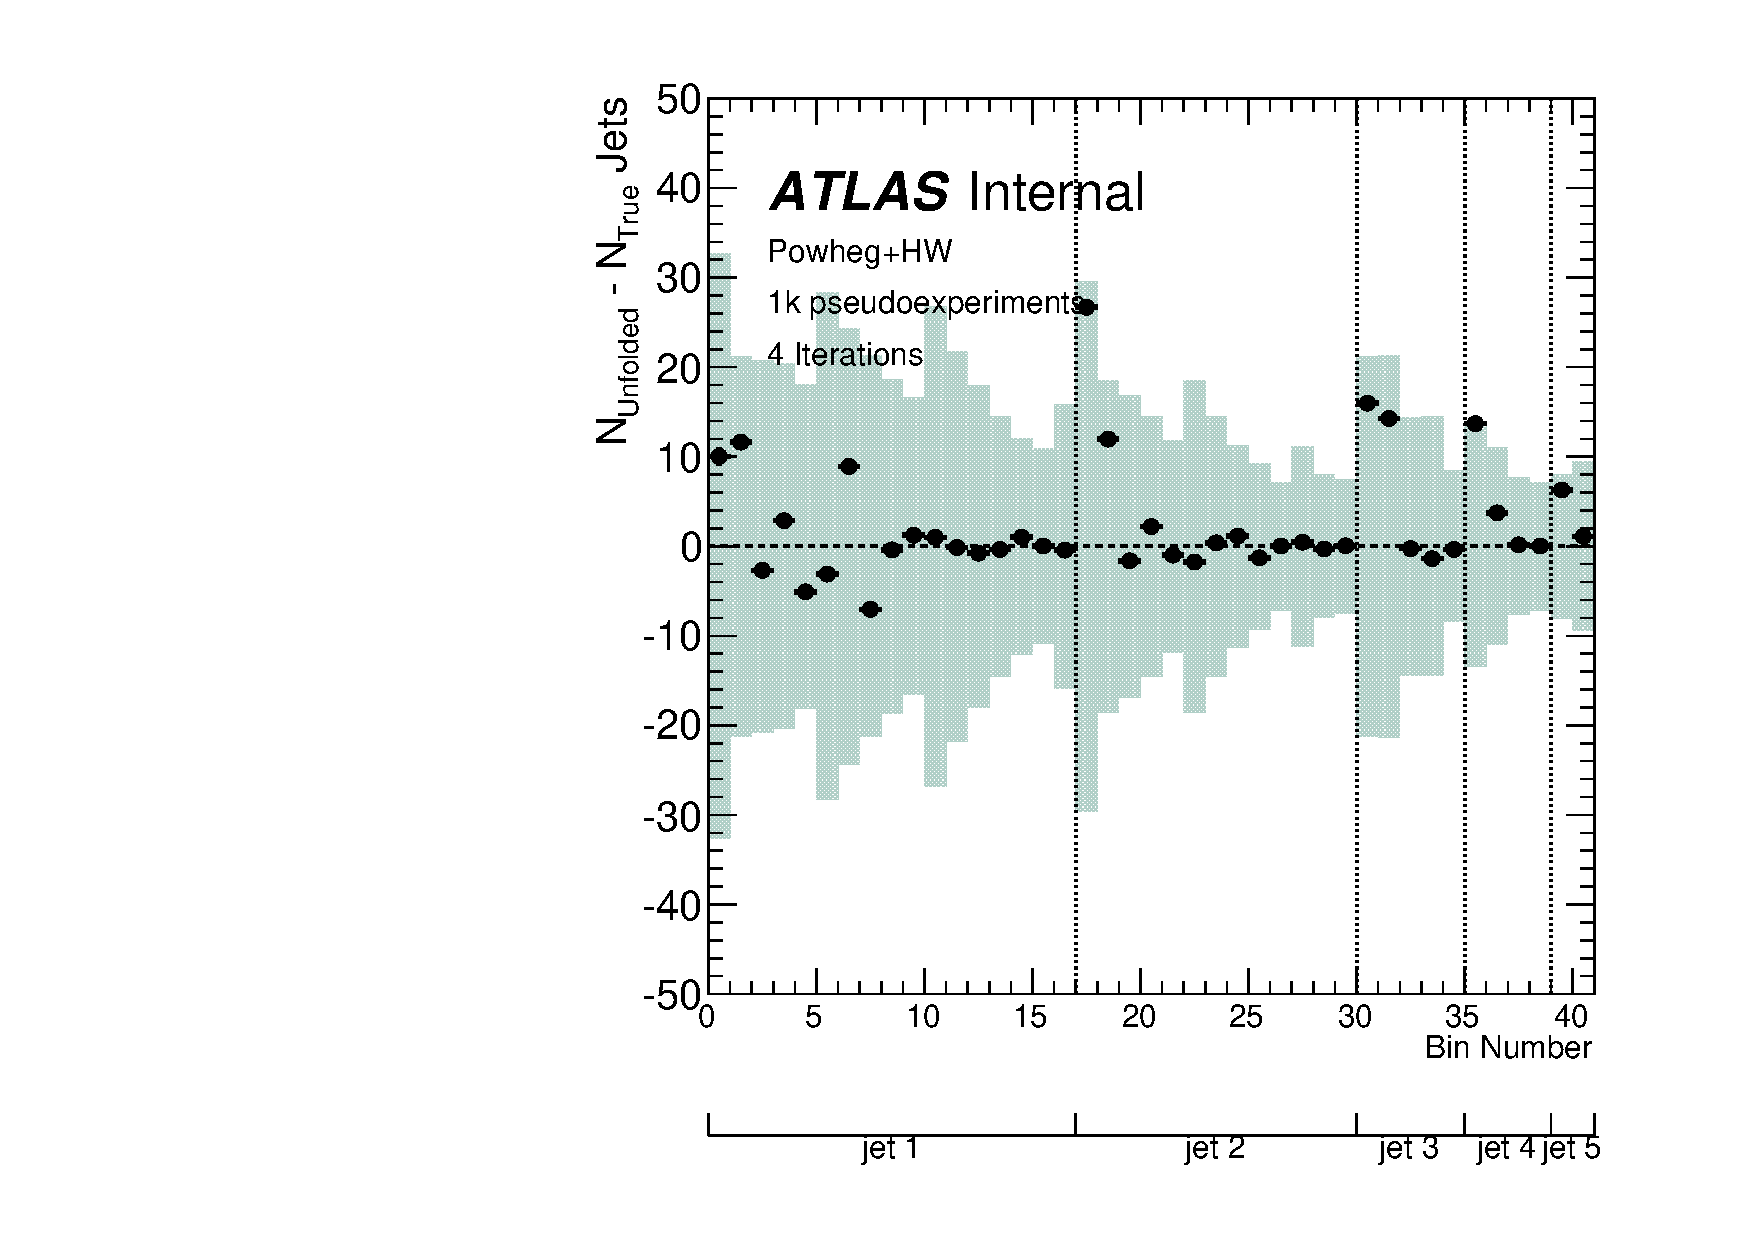
\includegraphics[width=\textwidth]{fig/Stress/105860atlfast/Bias4Iterations.pdf}
\end{subfigure}

\caption{Bias distribution for pseudoexperiments constructed from \pow+\hw simulation unfolded against a matrix filled with the baseline simulation. One thousand pseudoexperiments, each the size of the events in data, are selected from the sample and unfolded. The Bayesian unfolding method with various numbers of iterations is used. Each bin of the distribution over the pseudoexperiments is fit with a gaussian. The black points show the fitted mean of each bin and the blue band shows the fitted sigma. }
\label{fig:powhwbias}
\end{figure}

\clearpage


%\section{Bias \hdamp}
\begin{figure}
\begin{subfigure}[]{0.5\textwidth}
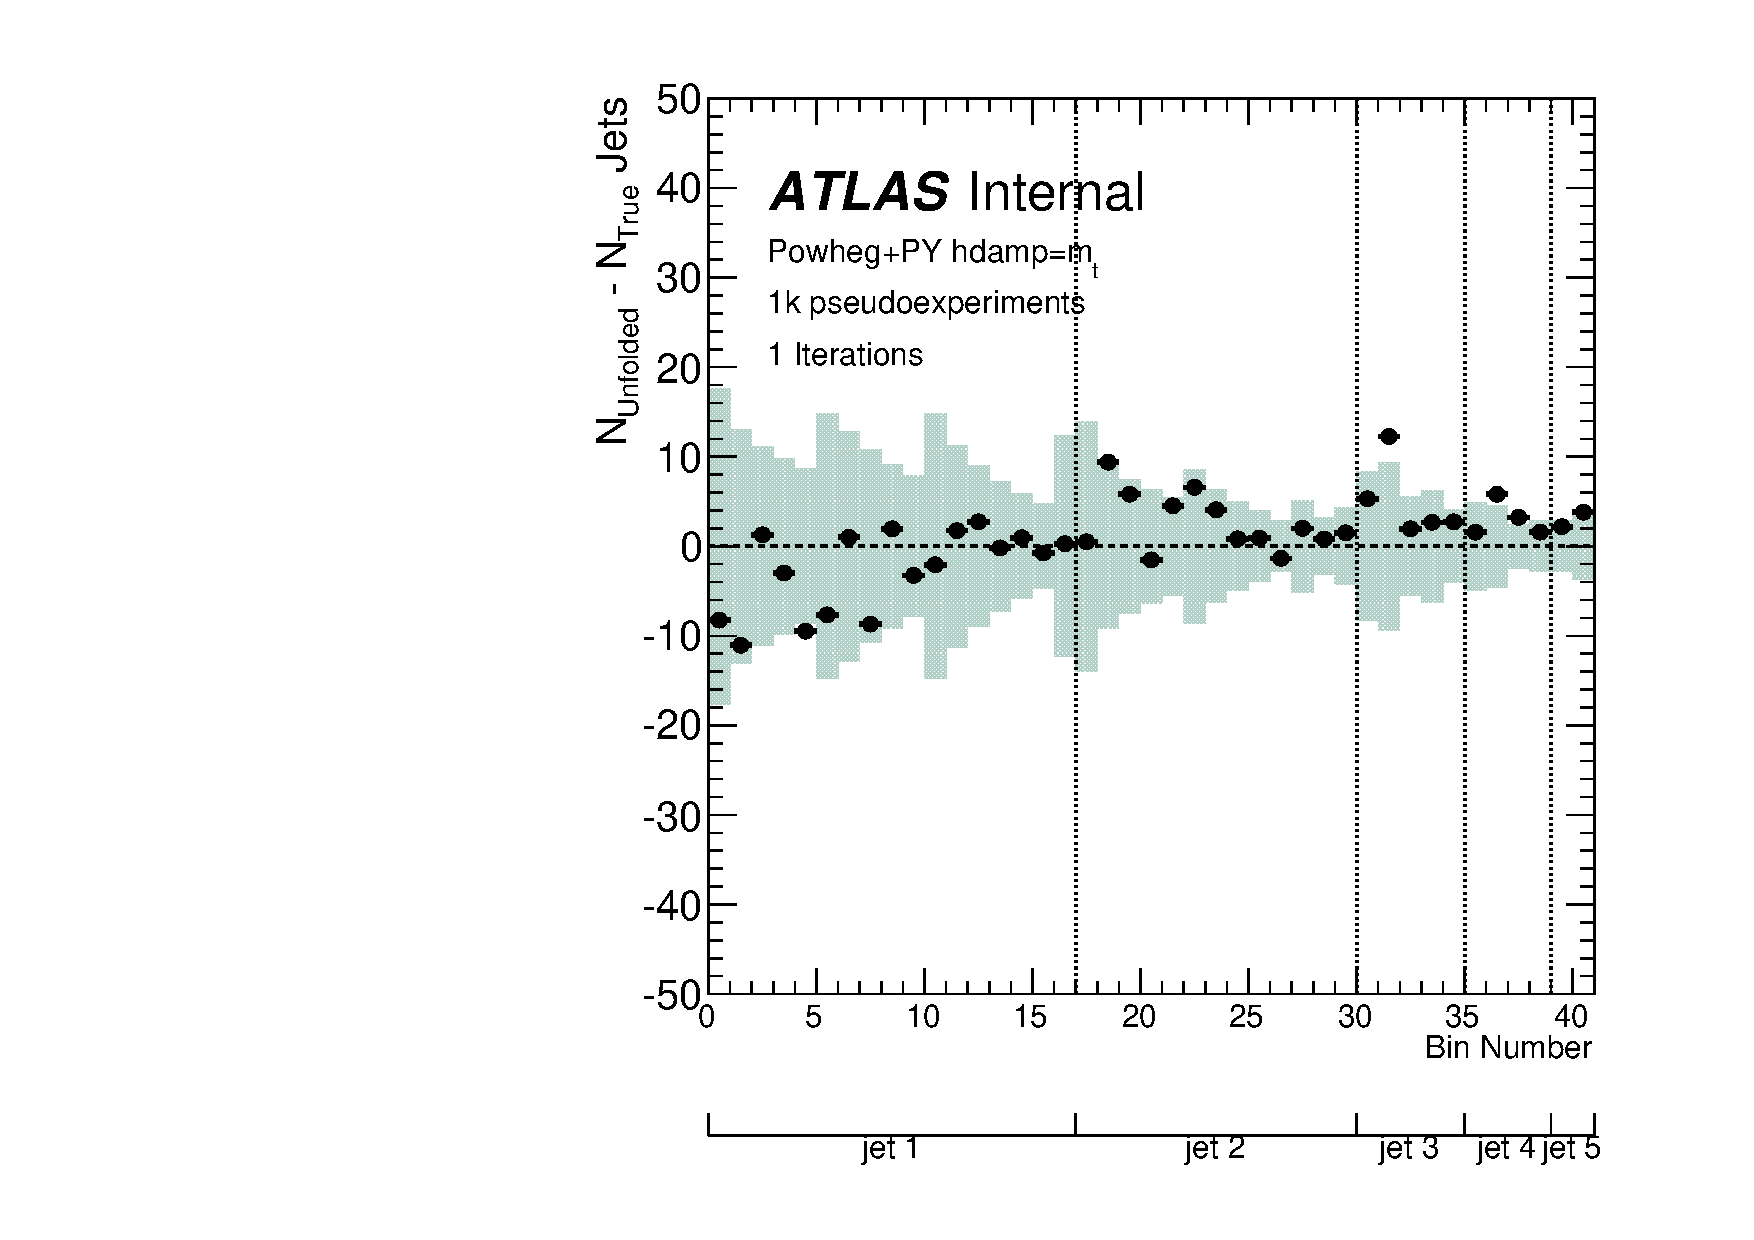
\includegraphics[width=\textwidth]{fig/Stress/110404atlfast/Bias1Iterations.pdf}
\end{subfigure}
~
\begin{subfigure}[]{0.5\textwidth}
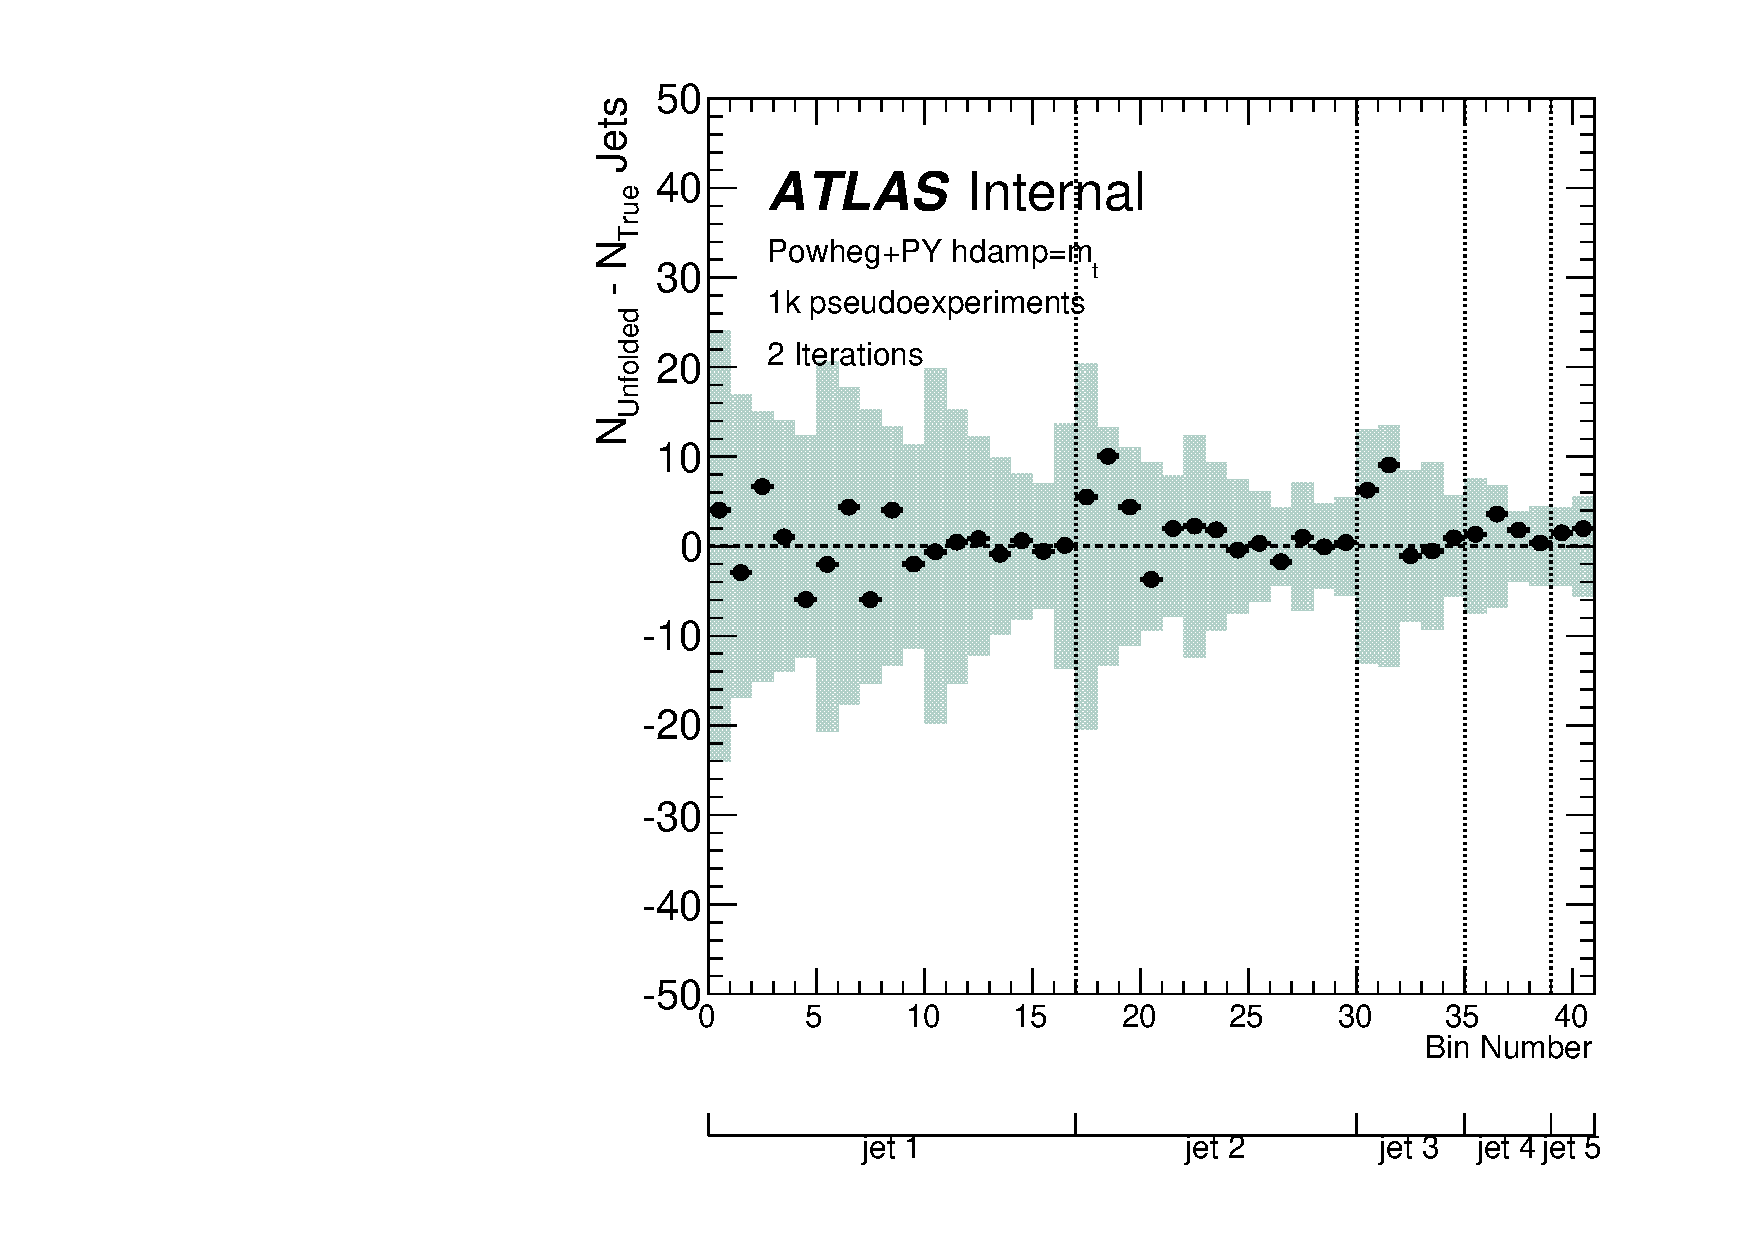
\includegraphics[width=\textwidth]{fig/Stress/110404atlfast/Bias2Iterations.pdf}
\end{subfigure}
\\
\begin{subfigure}[]{0.5\textwidth}
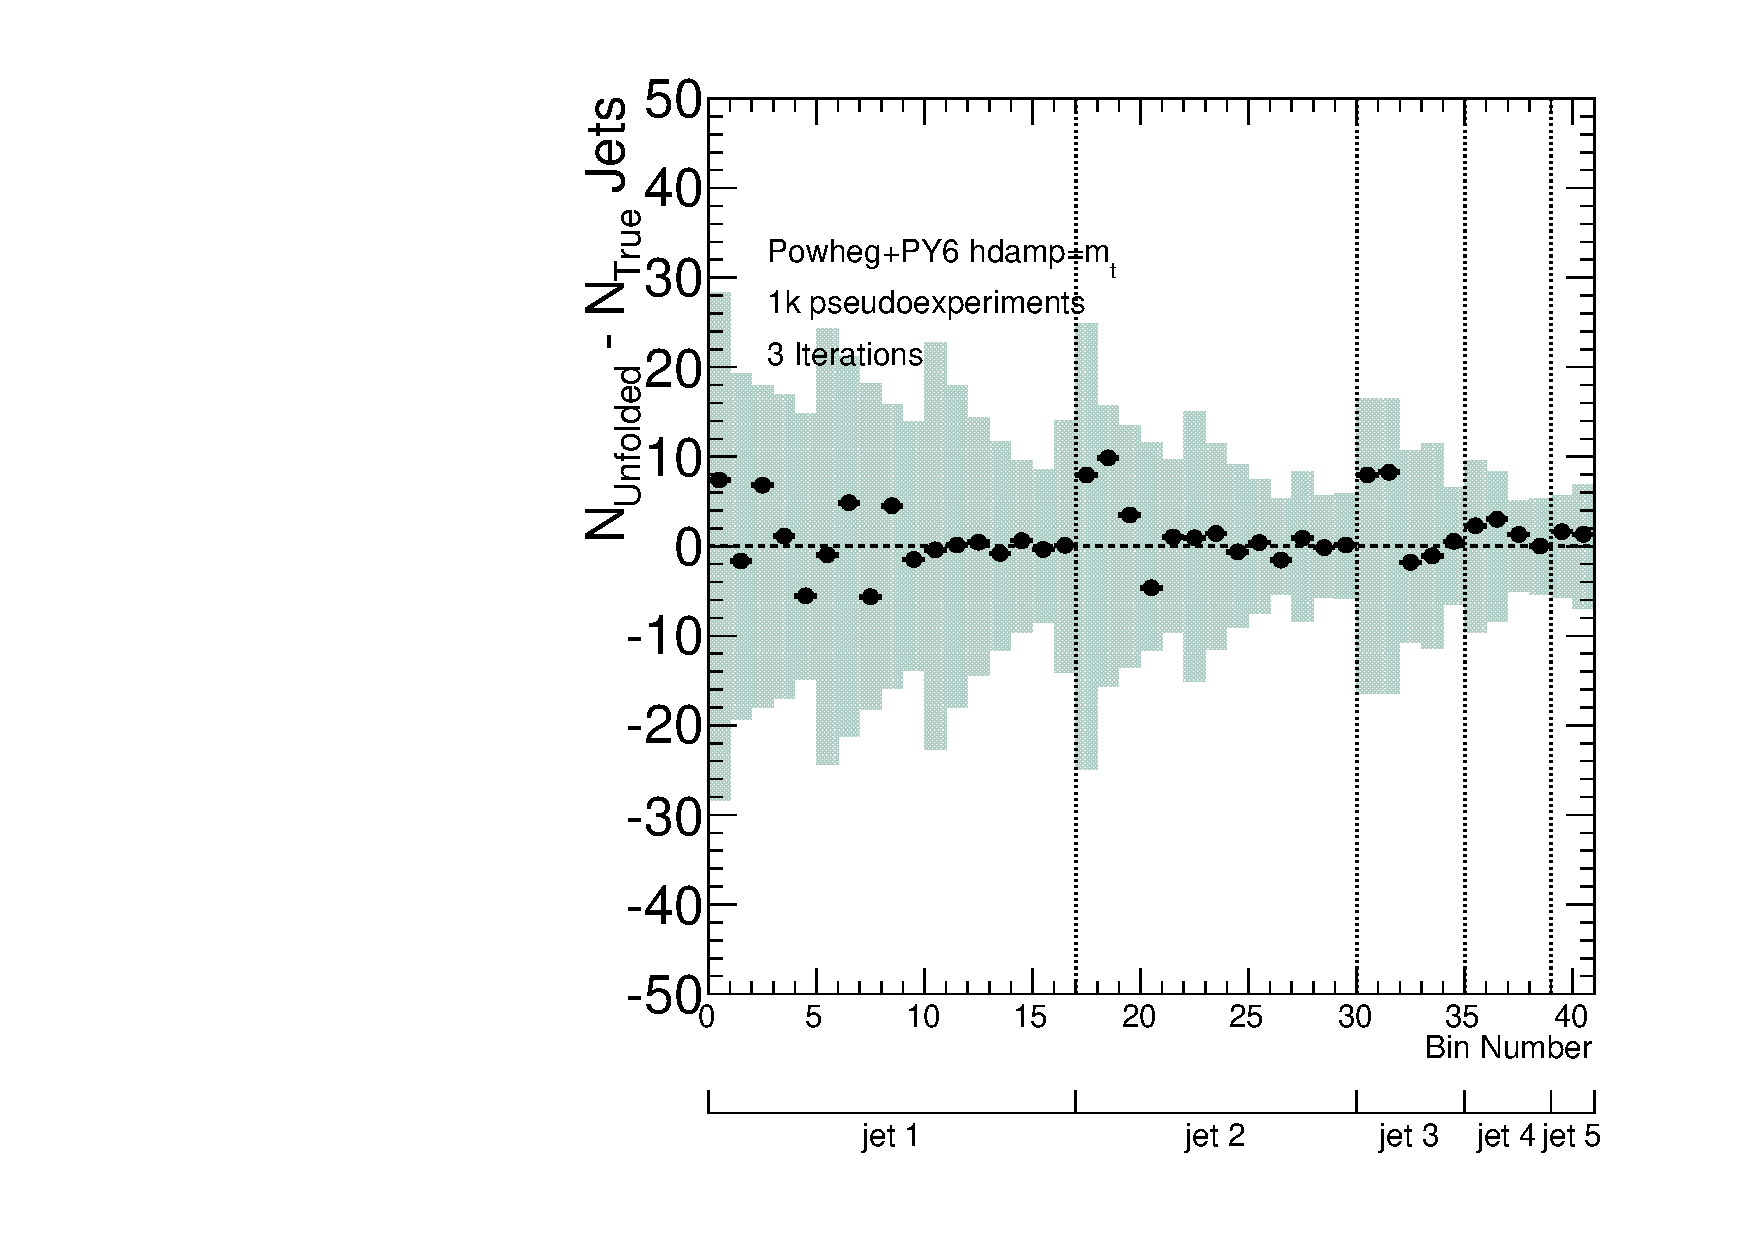
\includegraphics[width=\textwidth]{fig/Stress/110404atlfast/Bias3Iterations.pdf}
\end{subfigure}
~
\begin{subfigure}[]{0.5\textwidth}
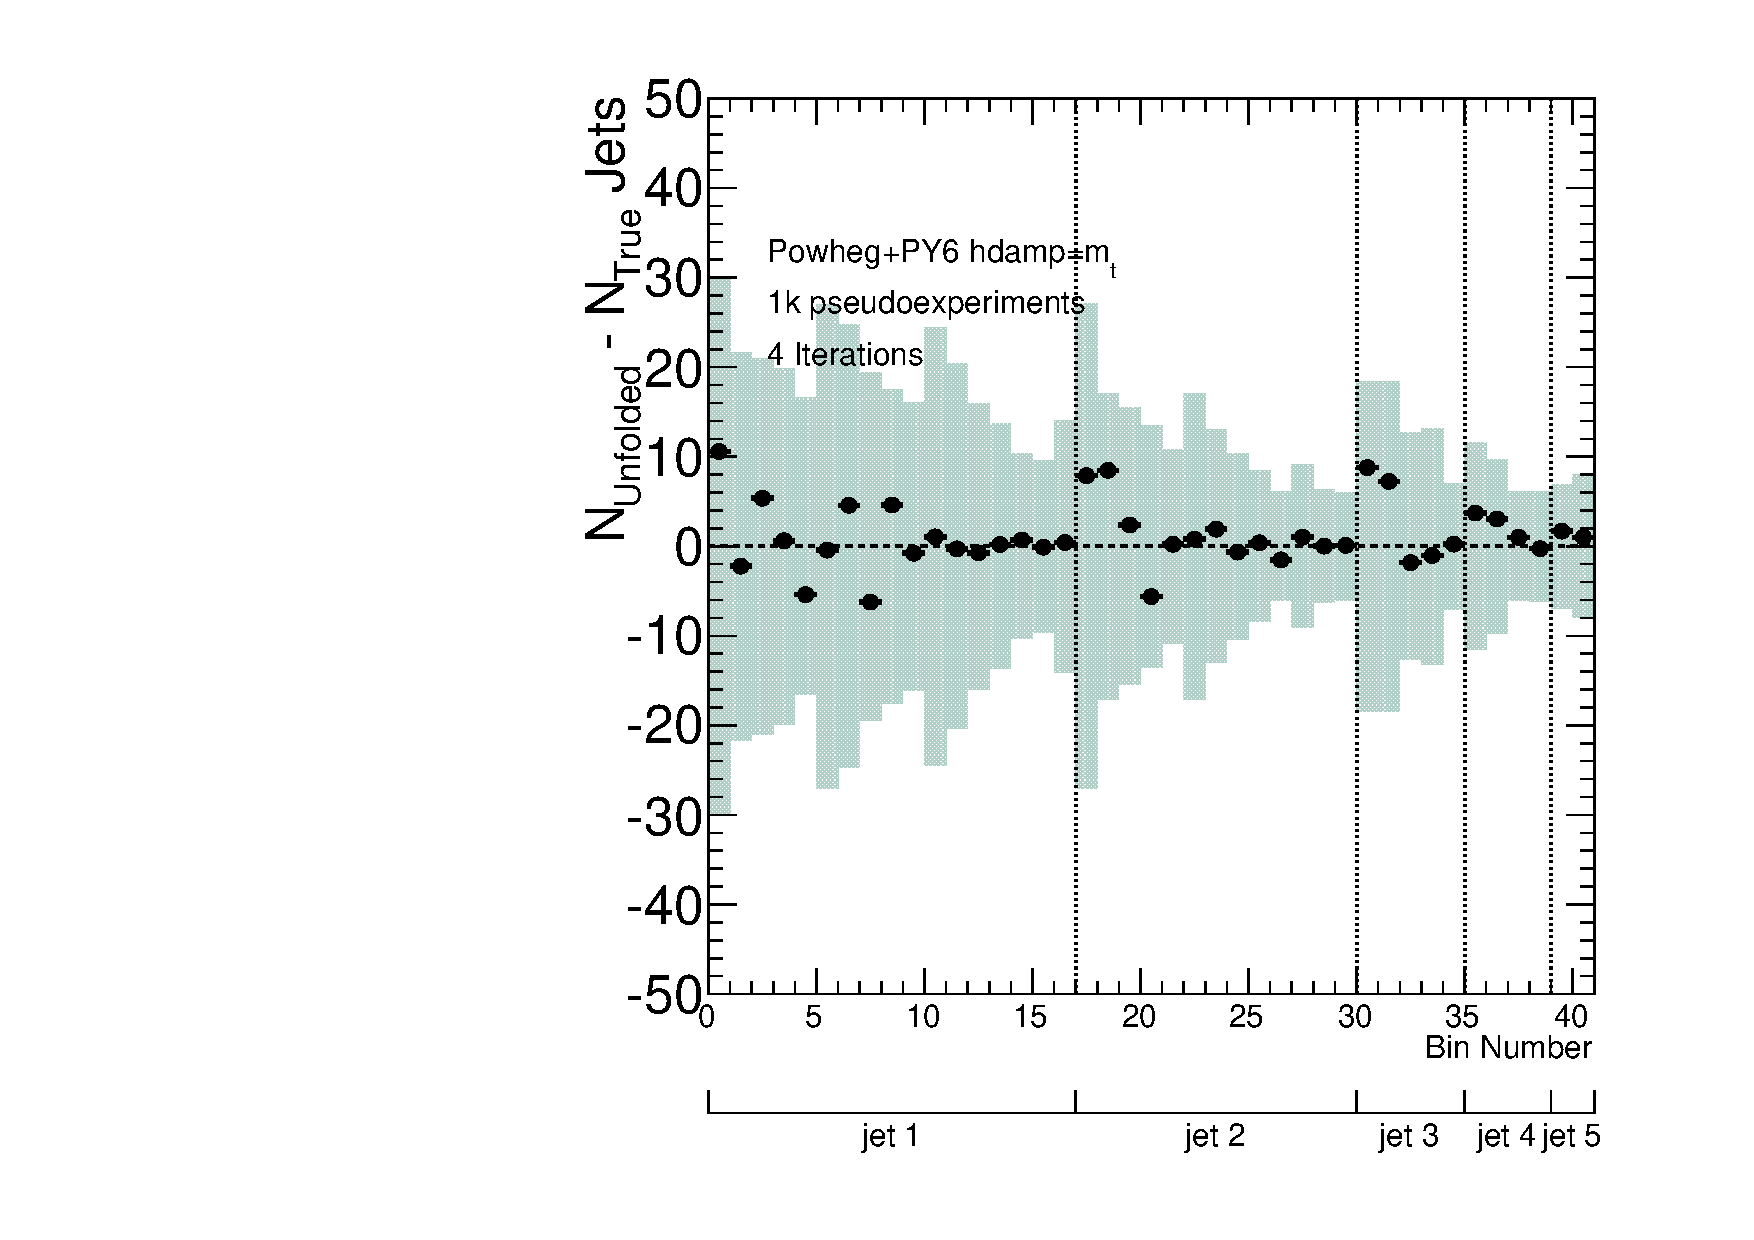
\includegraphics[width=\textwidth]{fig/Stress/110404atlfast/Bias4Iterations.pdf}
\end{subfigure}
\caption{Bias distribution for pseudoexperiments constructed from \newline \hdamp~ simulation unfolded against a matrix filled with the baseline simulation. One thousand pseudoexperiments, each the size of the events in data, are selected from the sample and unfolded. The Bayesian unfolding method with various numbers of iterations is used. Each bin of the distribution over the pseudoexperiments is fit with a gaussian. The black points show the fitted mean of each bin and the blue band shows the fitted sigma. }
\label{fig:hdampbias}
\end{figure}
\clearpage
%\section{Bias \peight}
\begin{figure}
\begin{subfigure}[]{0.5\textwidth}
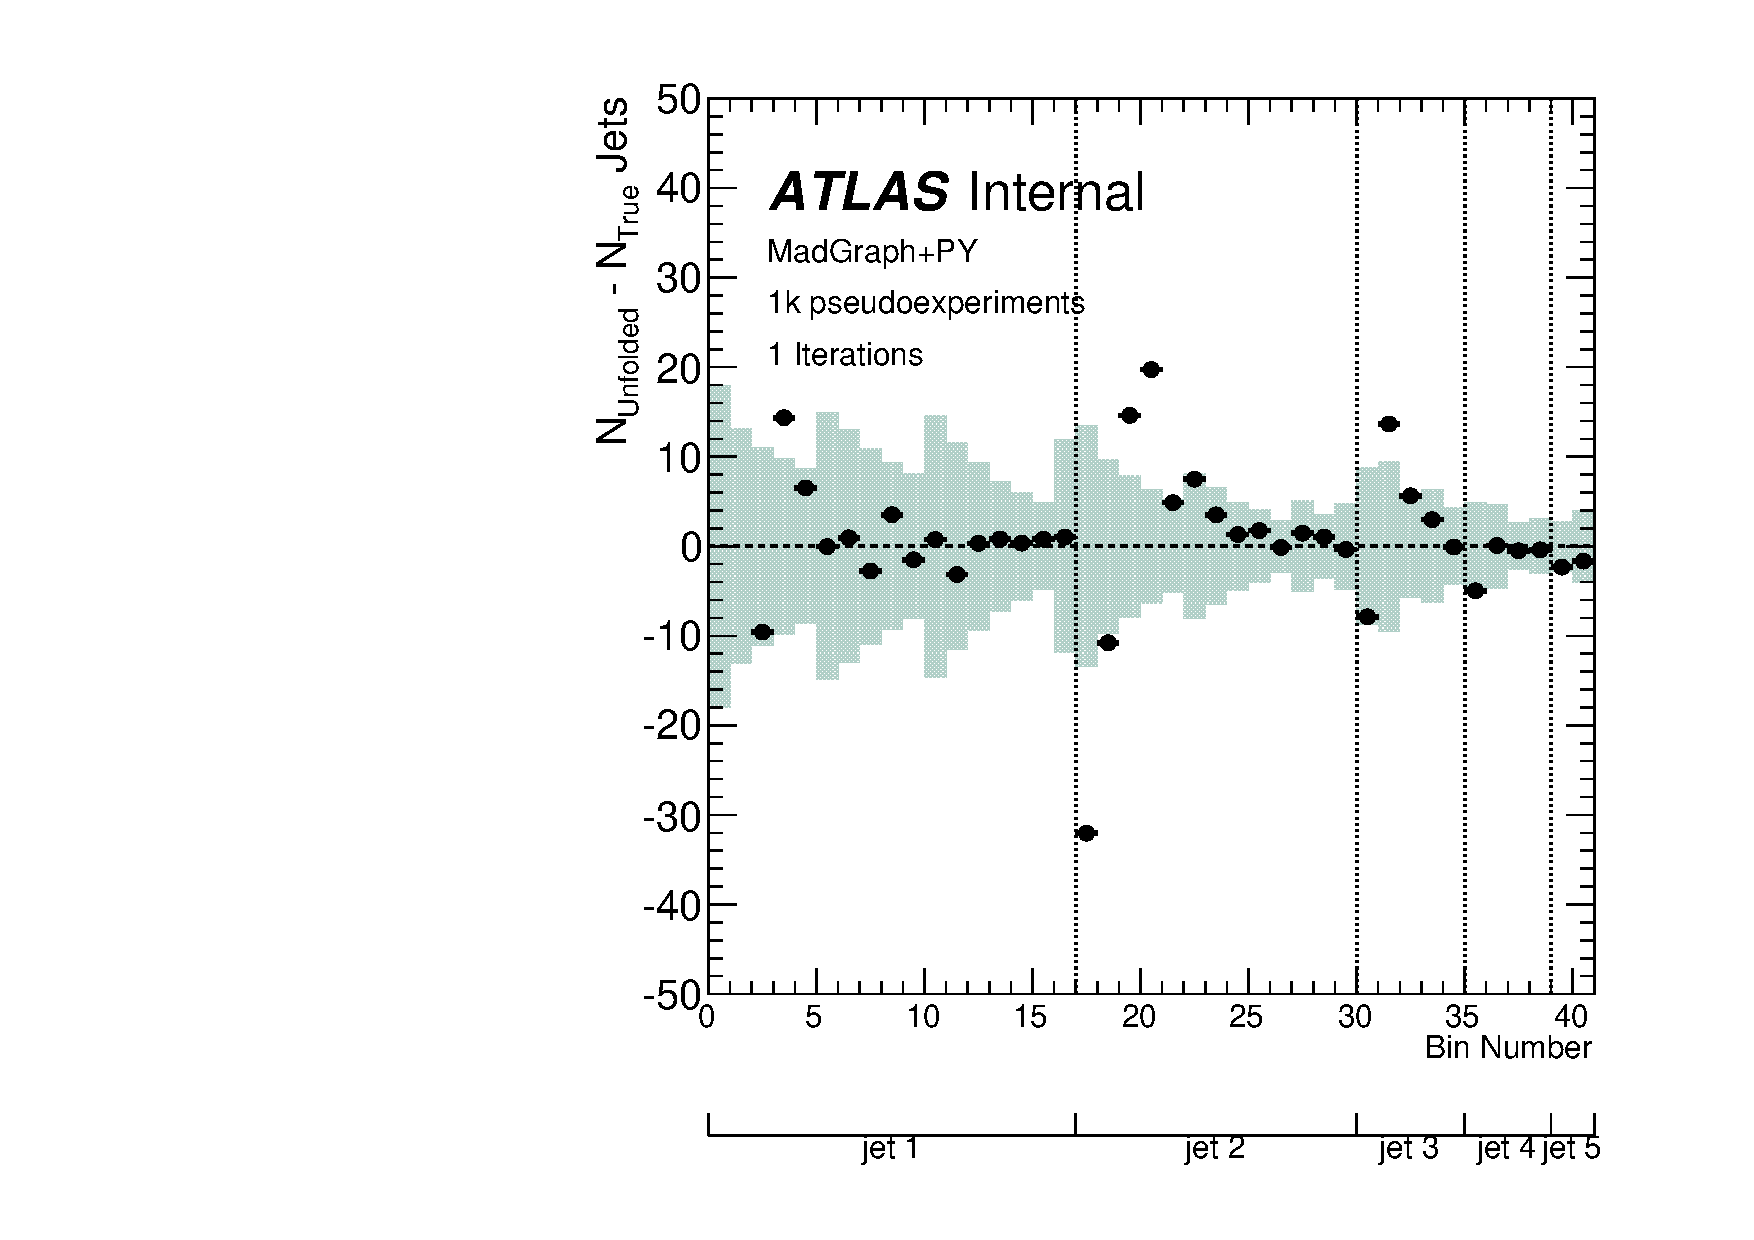
\includegraphics[width=\textwidth]{fig/Stress/110872atlfast/Bias1Iterations.pdf}
\end{subfigure}
~
\begin{subfigure}[]{0.5\textwidth}
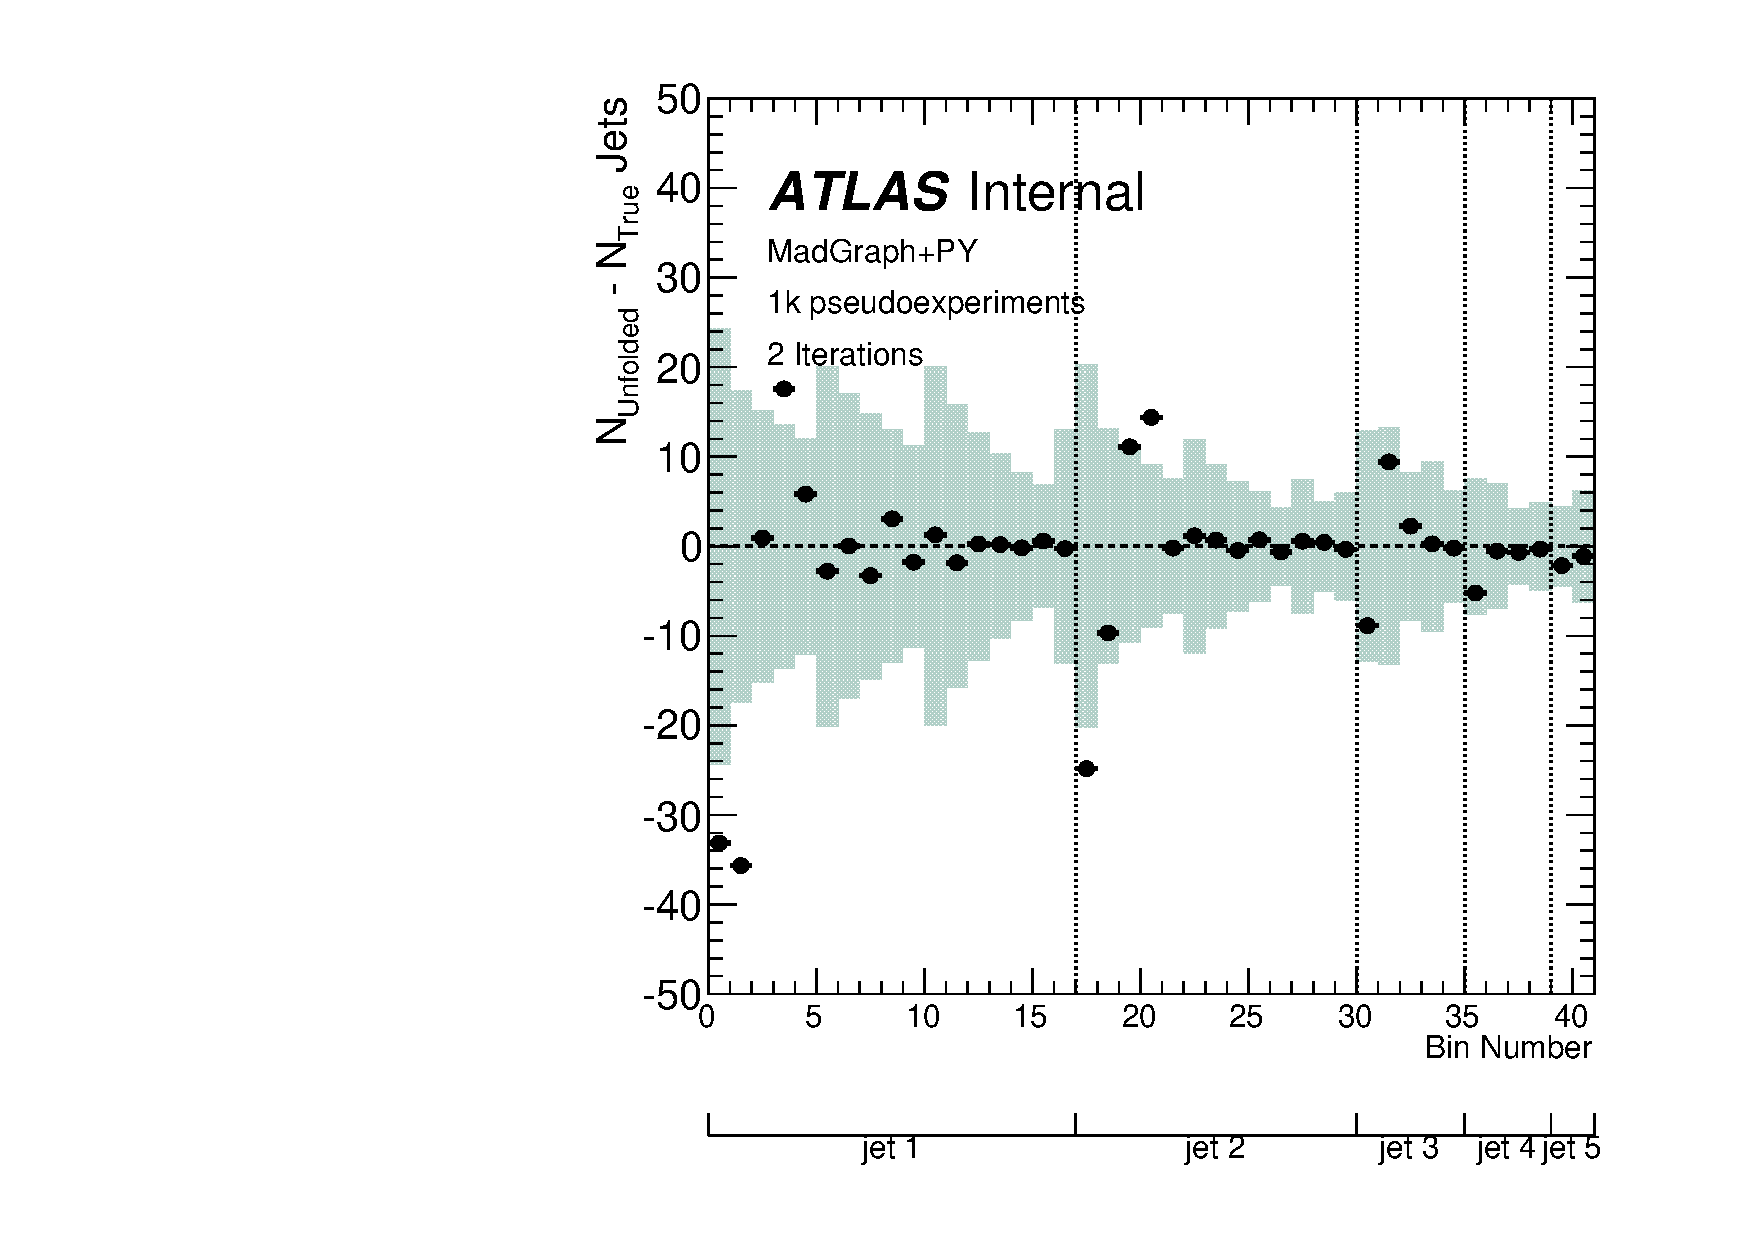
\includegraphics[width=\textwidth]{fig/Stress/110872atlfast/Bias2Iterations.pdf}
\end{subfigure}
\\
\begin{subfigure}[]{0.5\textwidth}
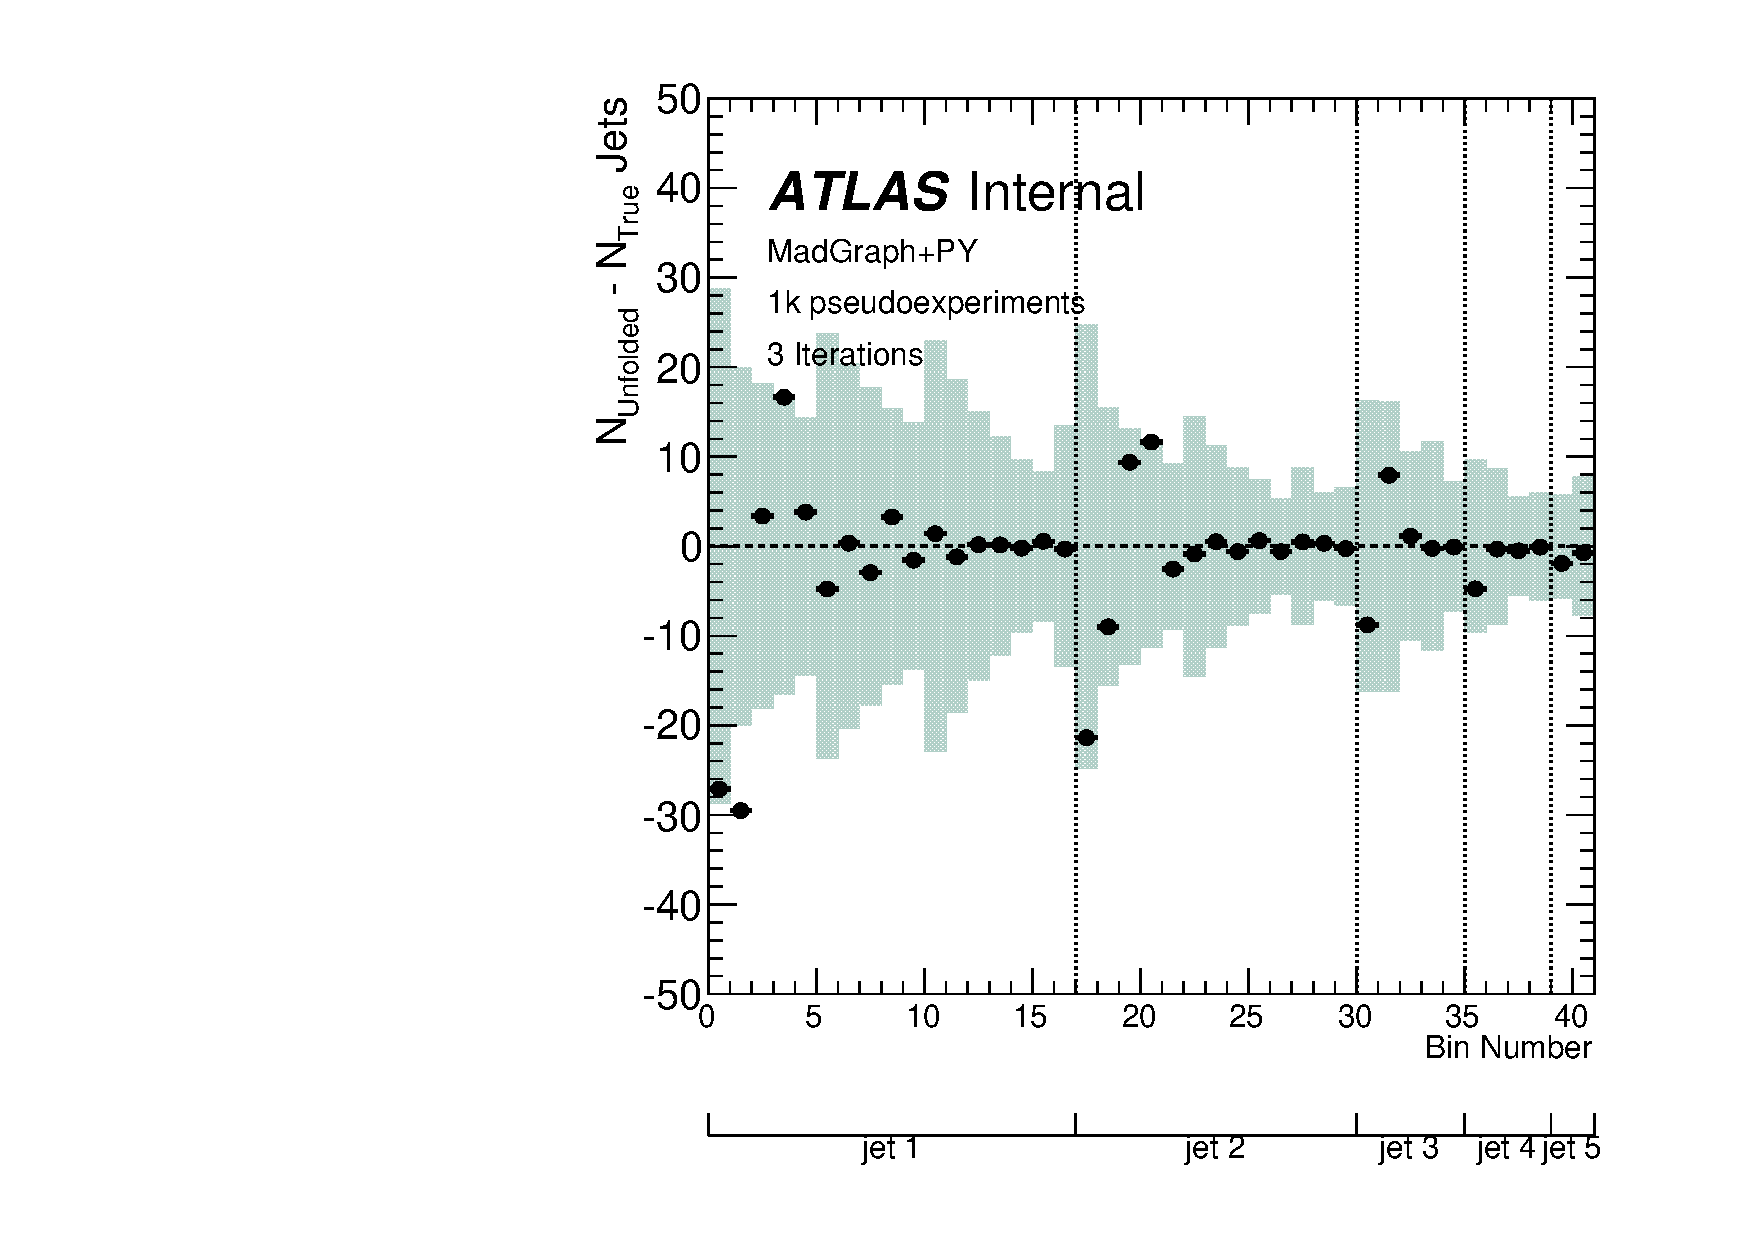
\includegraphics[width=\textwidth]{fig/Stress/110872atlfast/Bias3Iterations.pdf}
\end{subfigure}
~
\begin{subfigure}[]{0.5\textwidth}
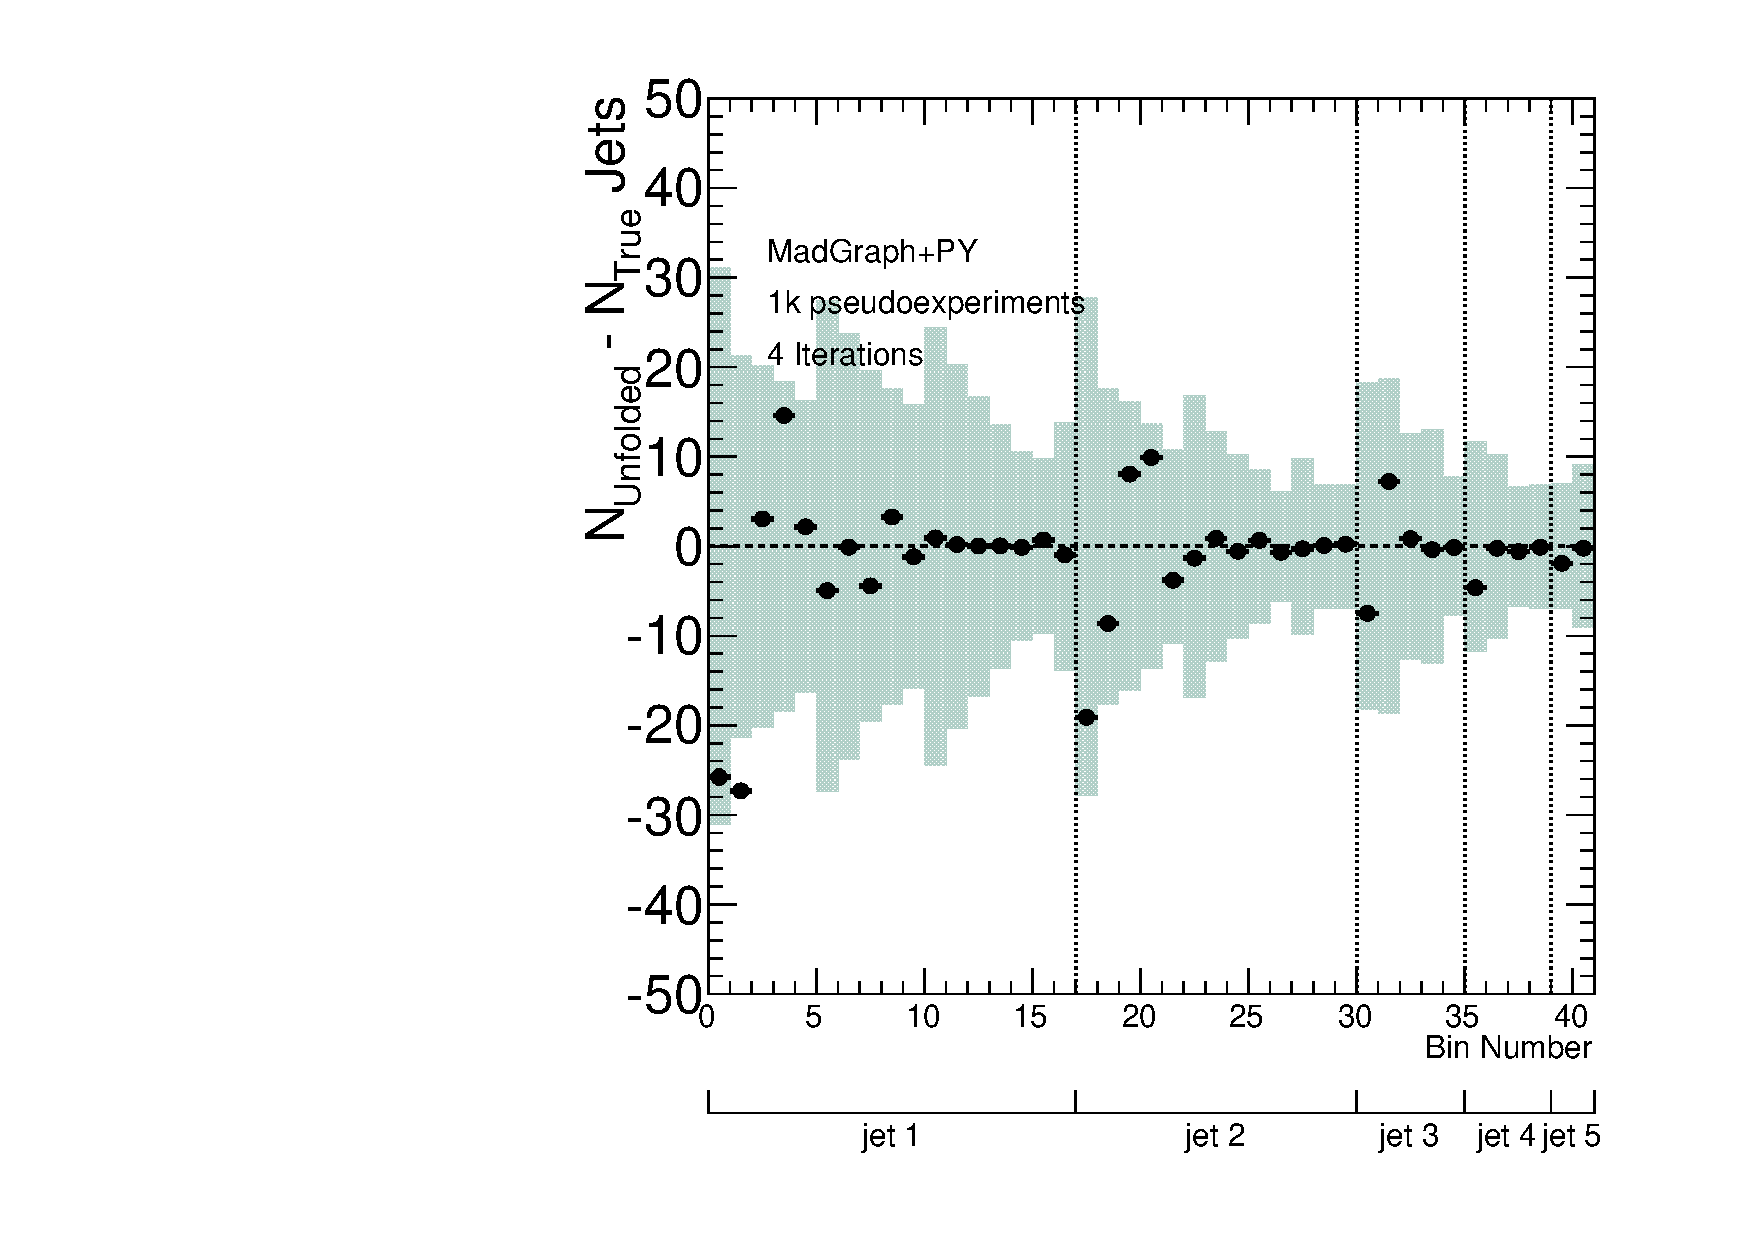
\includegraphics[width=\textwidth]{fig/Stress/110872atlfast/Bias4Iterations.pdf}
\end{subfigure}
\caption{Bias distribution for pseudoexperiments constructed from \newline \madpy\ simulation unfolded against a matrix filled with the baseline simulation. One thousand pseudoexperiments, each the size of the events in data, are selected from the sample and unfolded. The Bayesian unfolding method with various numbers of iterations is used. Each bin of the distribution over the pseudoexperiments is fit with a gaussian. The black points show the fitted mean of each bin and the blue band shows the fitted sigma.}
\label{fig:p8bias}
\end{figure}
\clearpage
%\section{Bias \powpy\ fullsim}
\begin{figure}
\begin{subfigure}[]{0.5\textwidth}
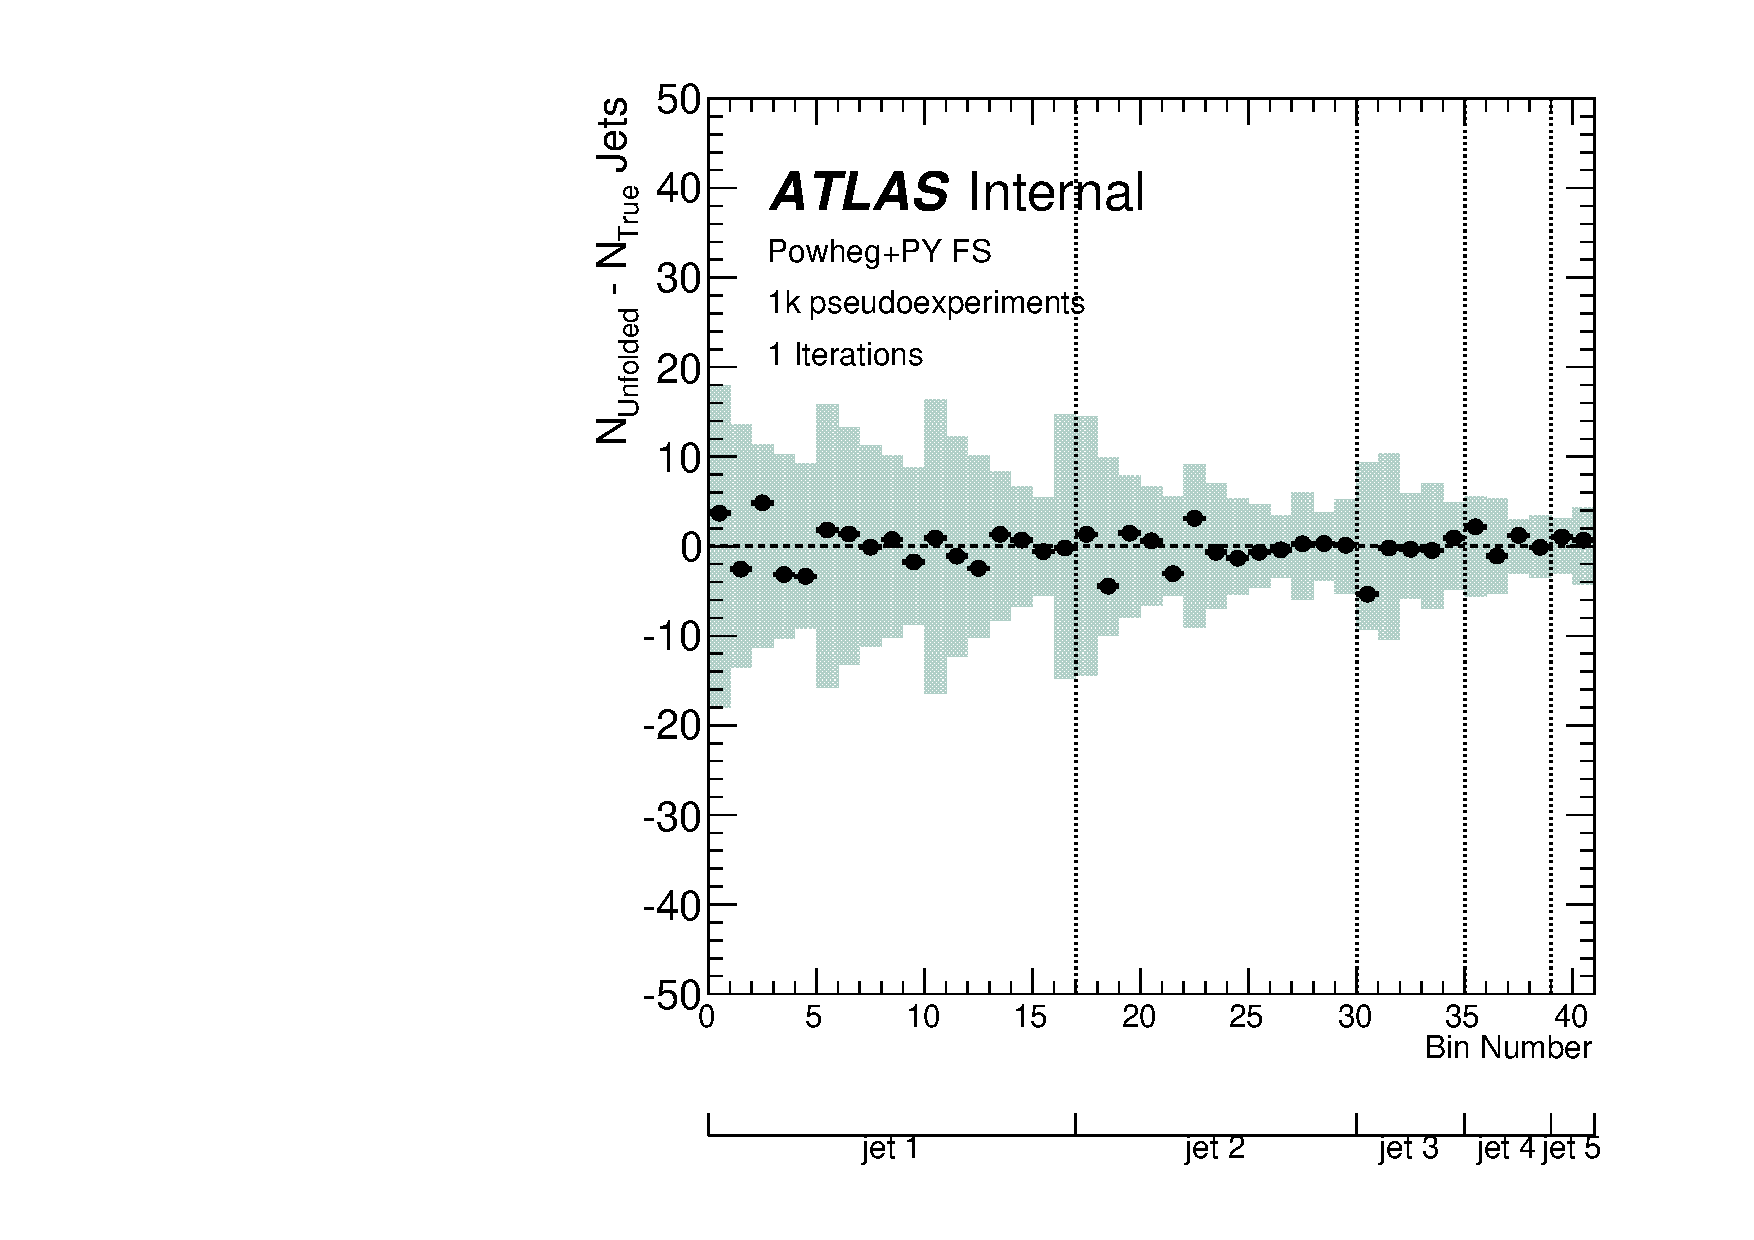
\includegraphics[width=\textwidth]{fig/Stress/117050fullsim/Bias1Iterations.pdf}
\end{subfigure}
~
\begin{subfigure}[]{0.5\textwidth}
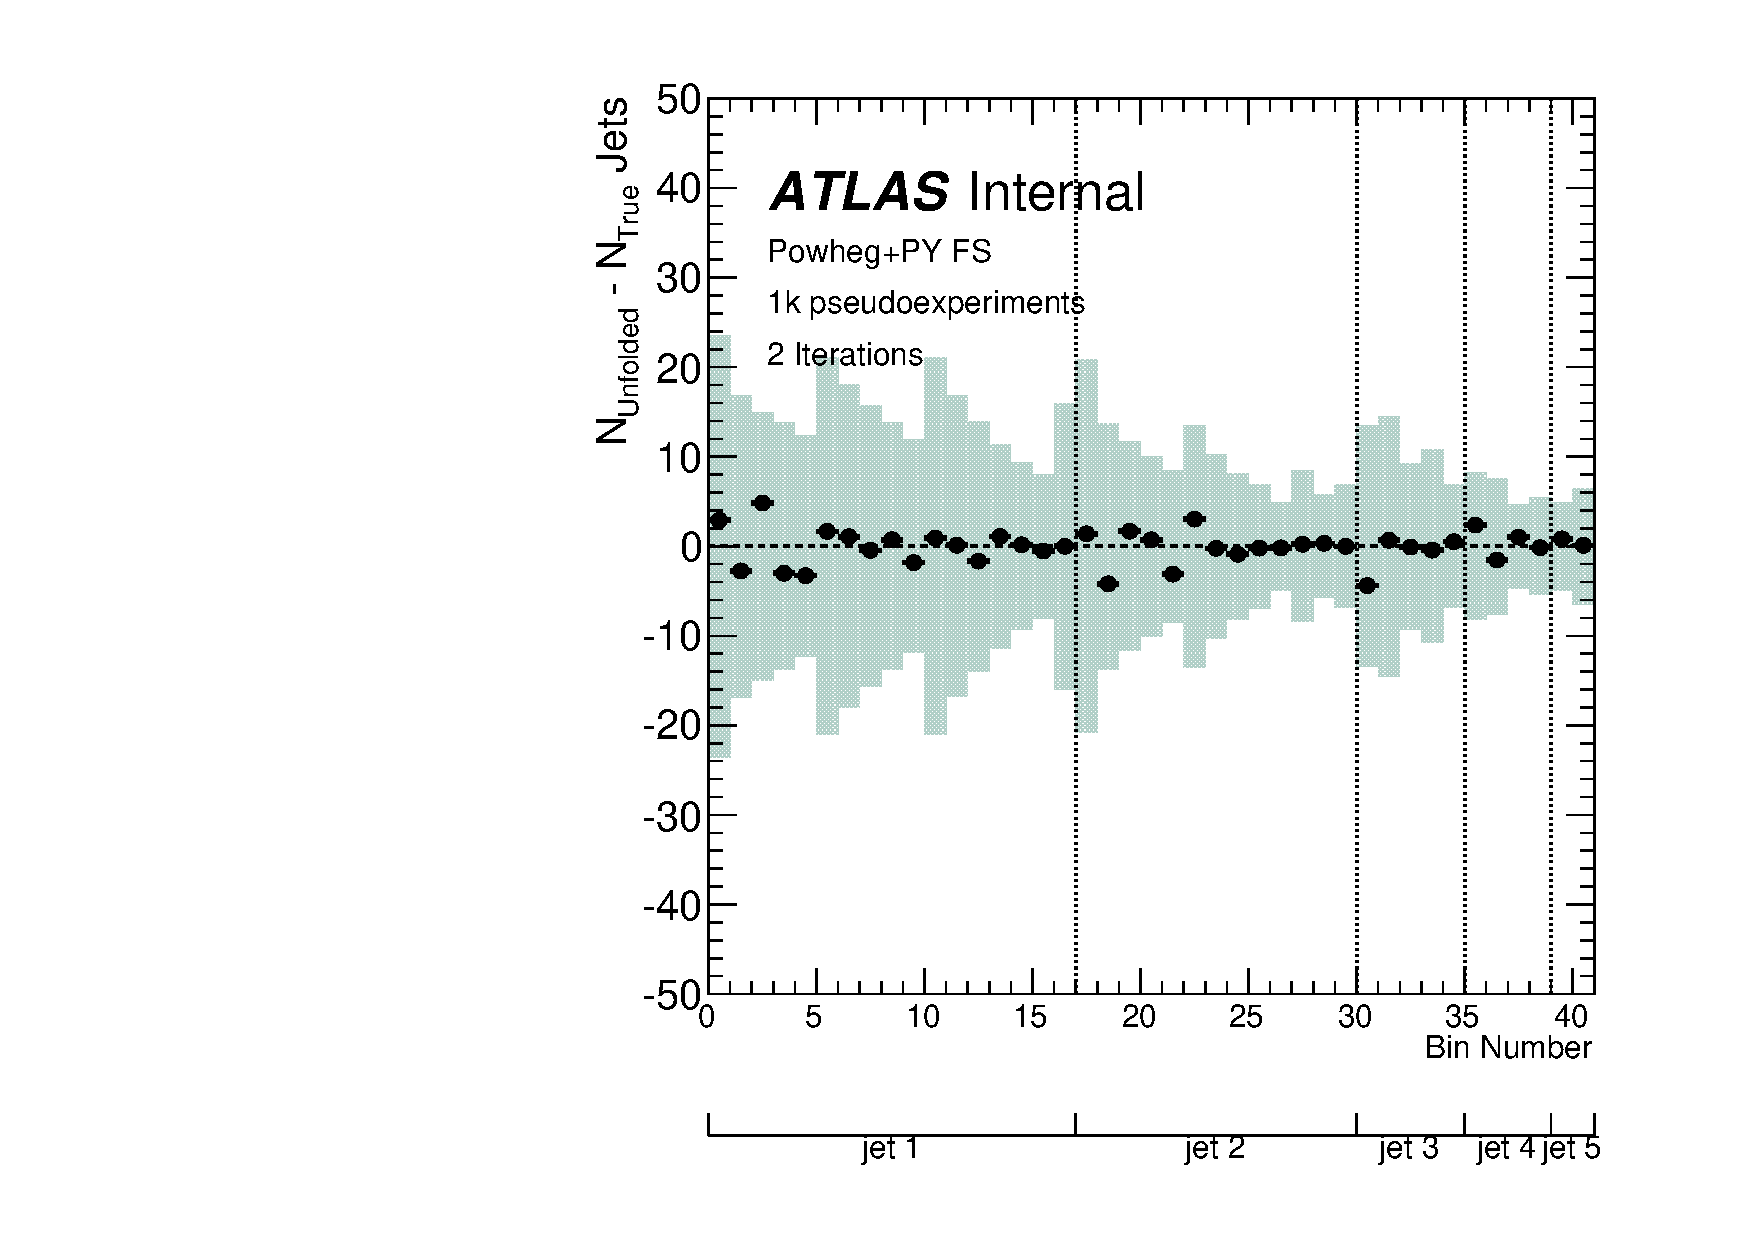
\includegraphics[width=\textwidth]{fig/Stress/117050fullsim/Bias2Iterations.pdf}
\end{subfigure}
\\
\begin{subfigure}[]{0.5\textwidth}
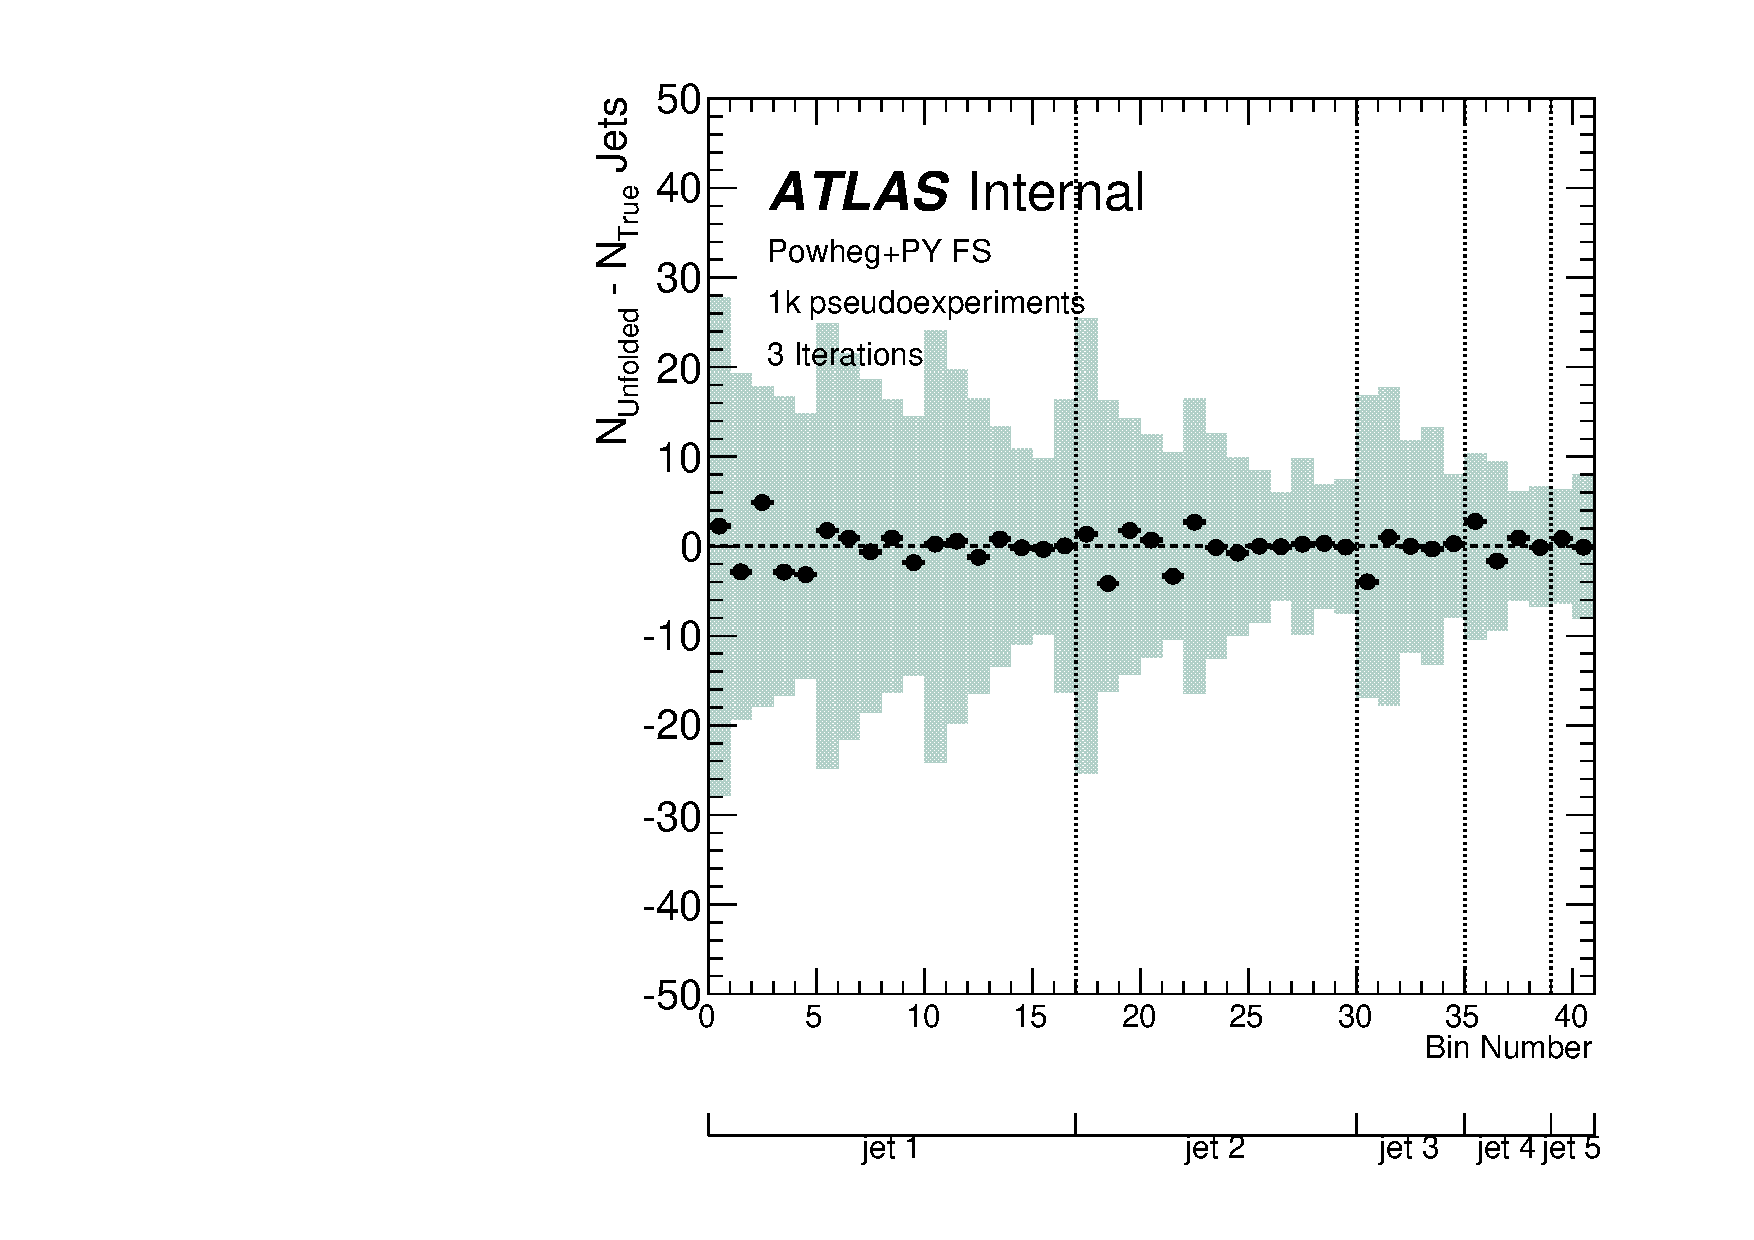
\includegraphics[width=\textwidth]{fig/Stress/117050fullsim/Bias3Iterations.pdf}
\end{subfigure}
~
\begin{subfigure}[]{0.5\textwidth}
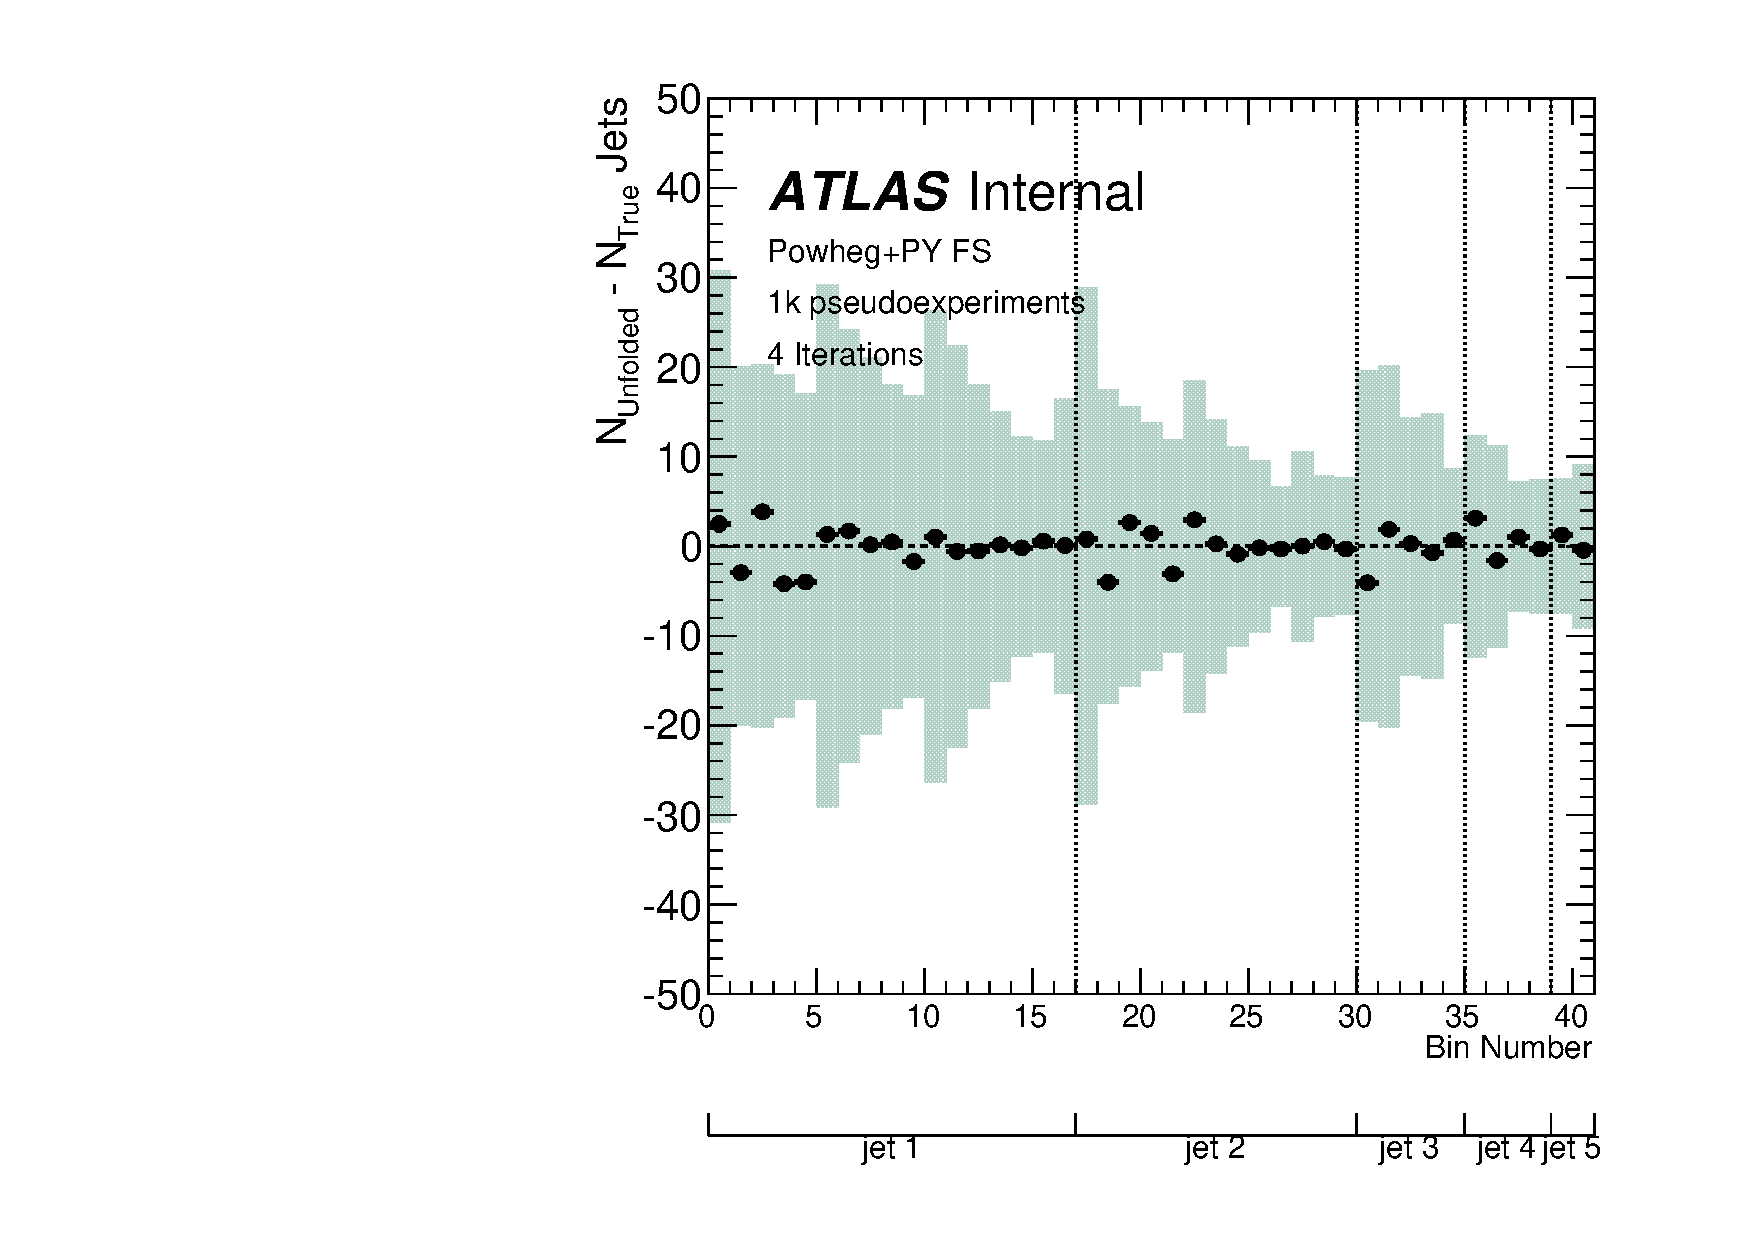
\includegraphics[width=\textwidth]{fig/Stress/117050fullsim/Bias4Iterations.pdf}
\end{subfigure}
\caption{Bias distribution for pseudoexperiments constructed from \newline \powpy\ fullsim simulation unfolded against a matrix filled with the baseline simulation. One thousand pseudoexperiments, each the size of the events in data, are selected from the sample and unfolded. The Bayesian unfolding method with various numbers of iterations is used. Each bin of the distribution over the pseudoexperiments is fit with a gaussian. The black points show the fitted mean of each bin and the blue band shows the fitted sigma.}
\label{fig:fsbias}
\end{figure}
\clearpage
\begin{figure}
\begin{subfigure}[]{0.5\textwidth}
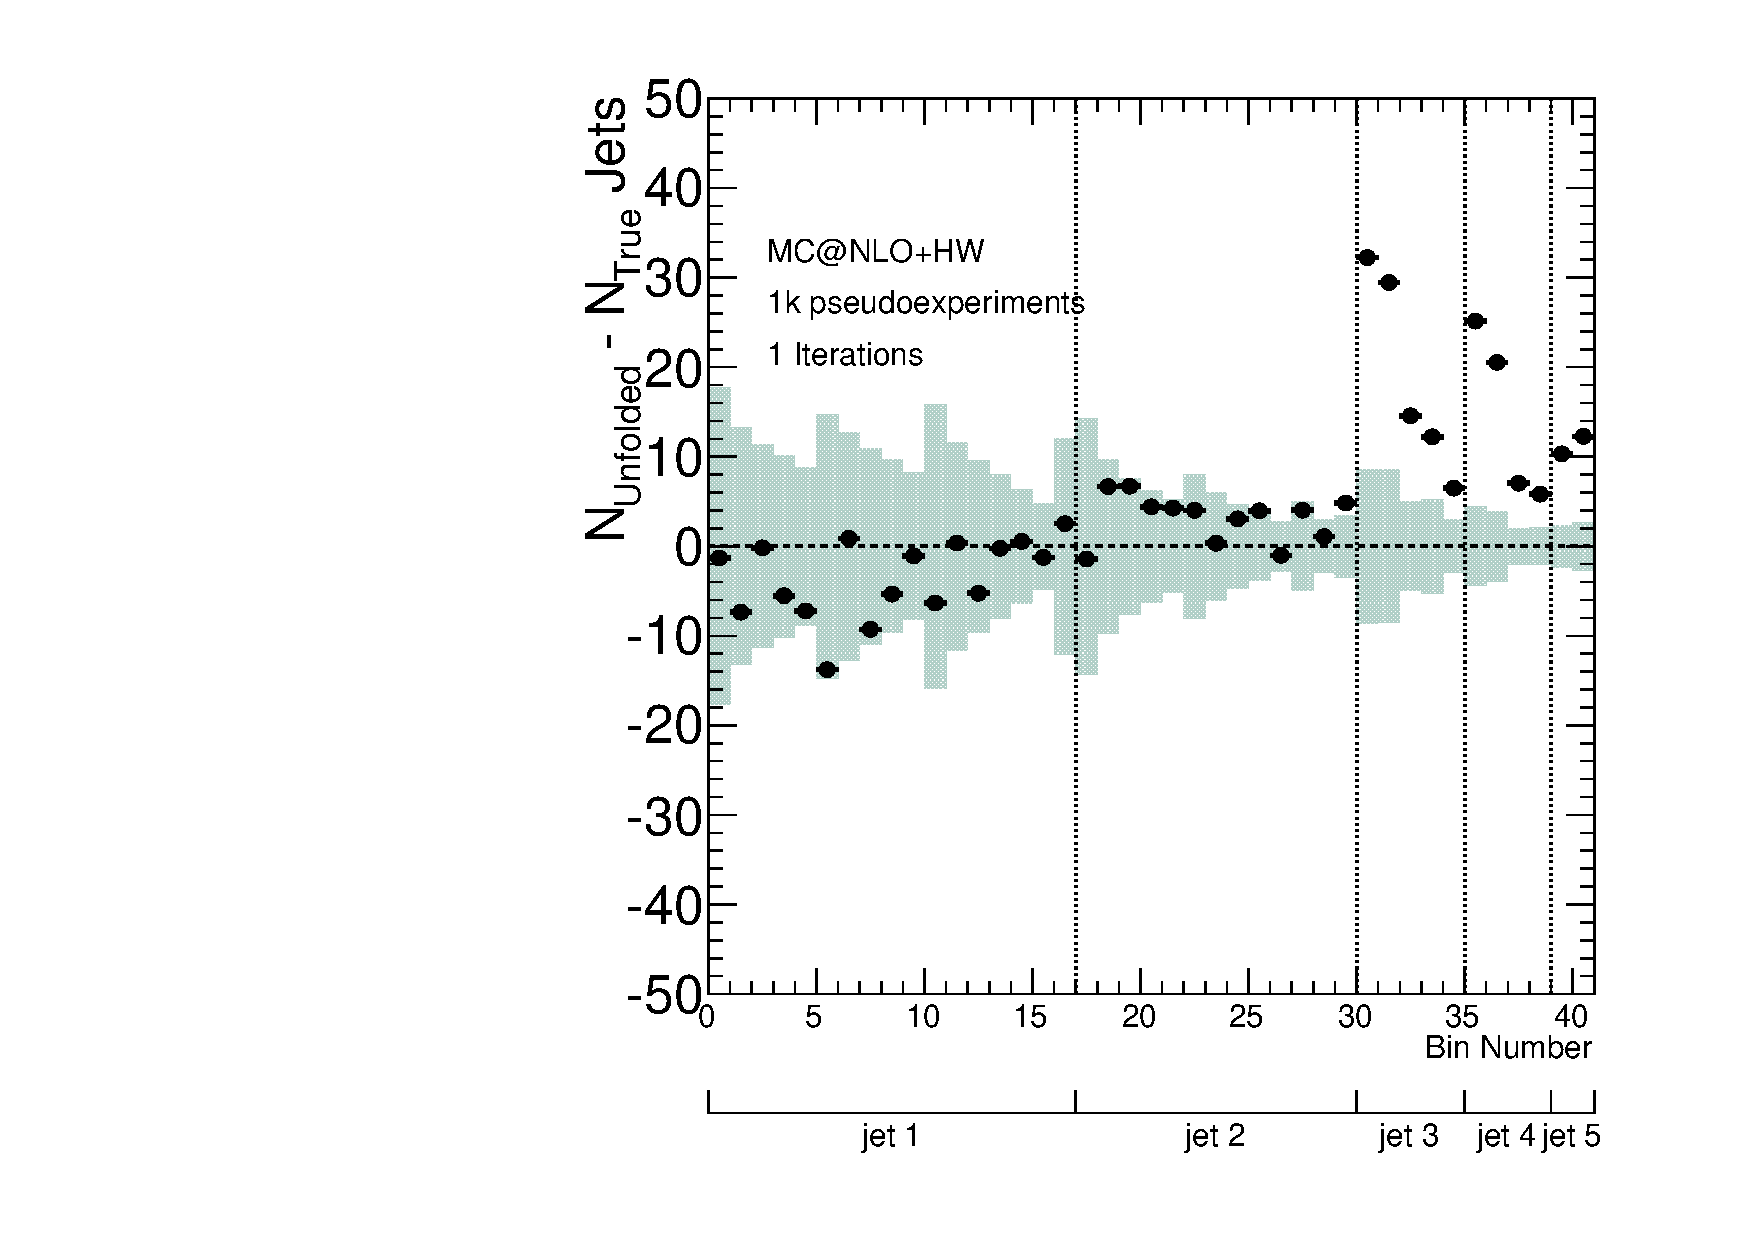
\includegraphics[width=\textwidth]{fig/Stress/105200atlfast/Bias1Iterations.pdf}
\end{subfigure}
\begin{subfigure}[]{0.5\textwidth}
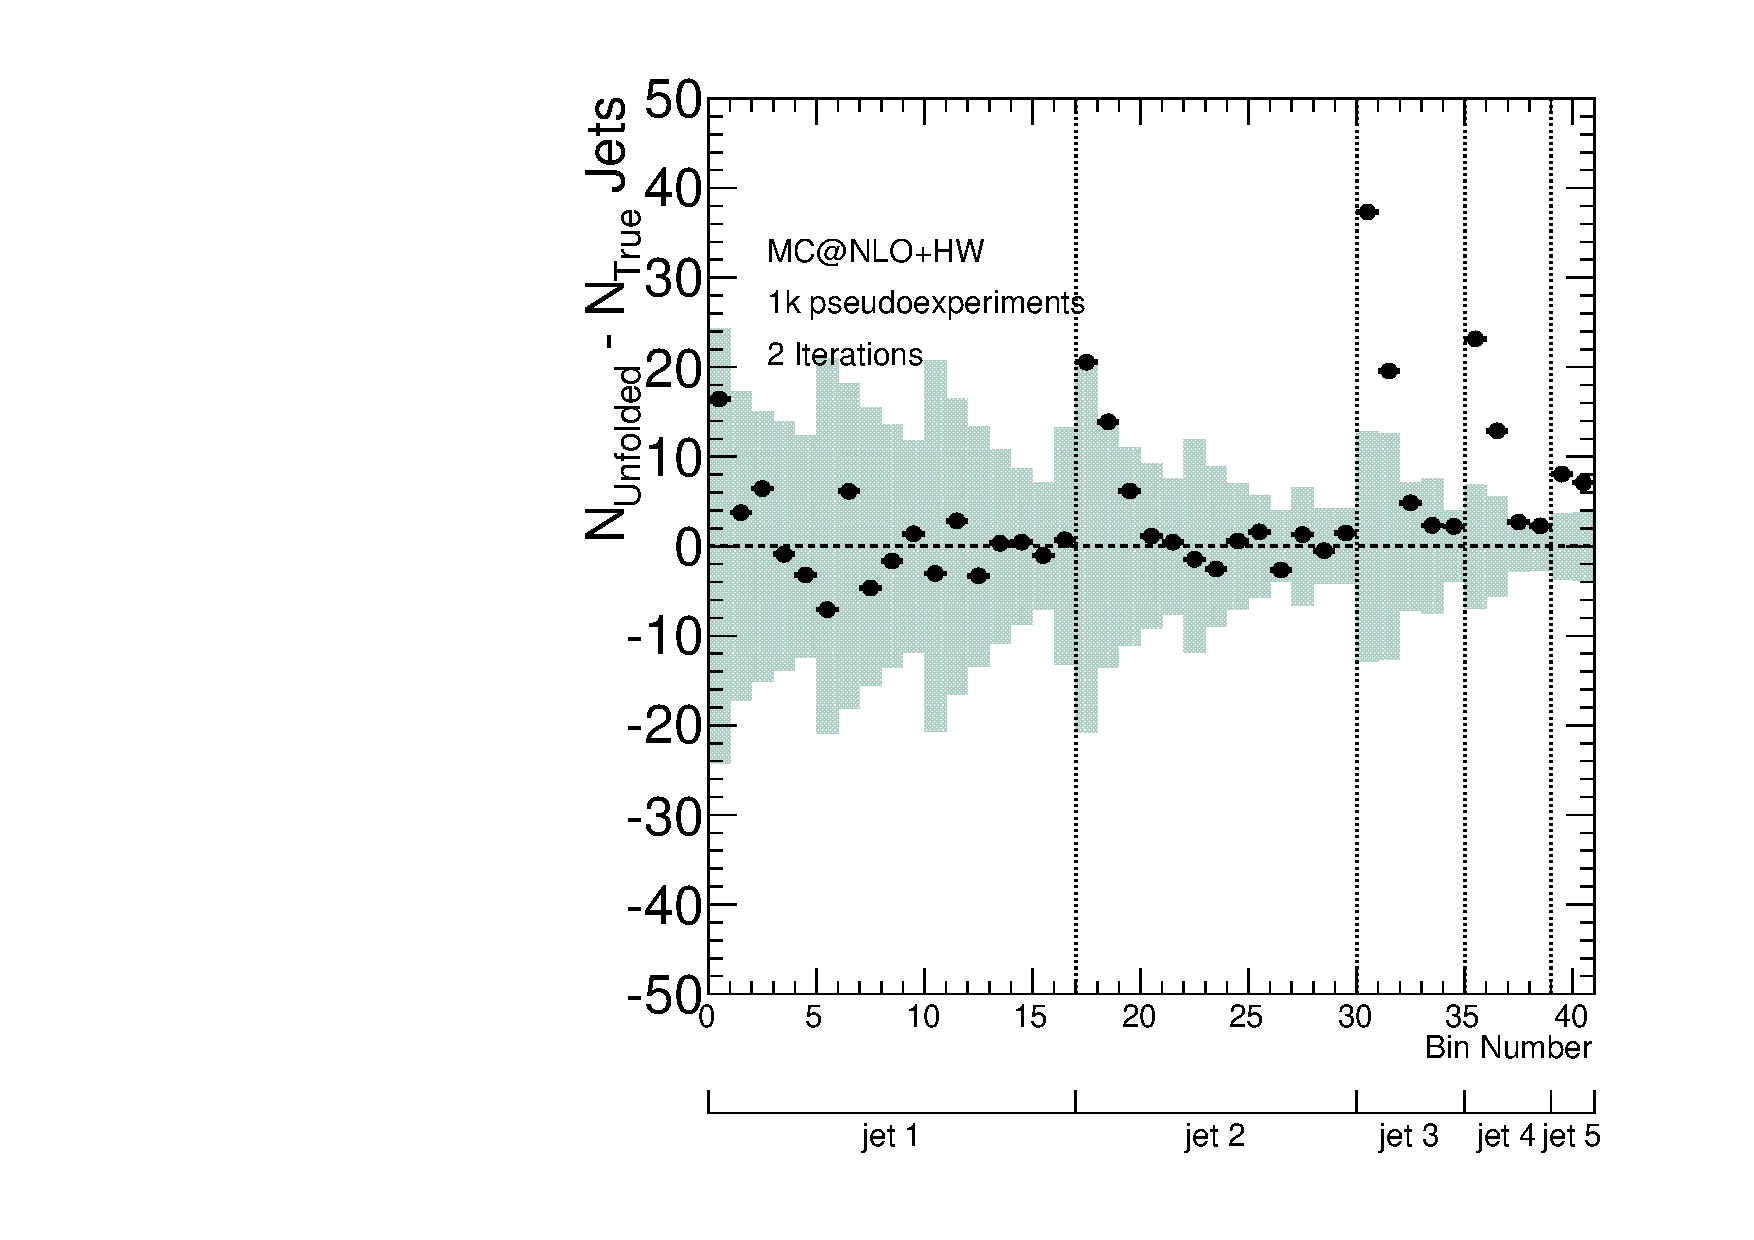
\includegraphics[width=\textwidth]{fig/Stress/105200atlfast/Bias2Iterations.pdf}
\end{subfigure}
\\
\begin{subfigure}[]{0.5\textwidth}
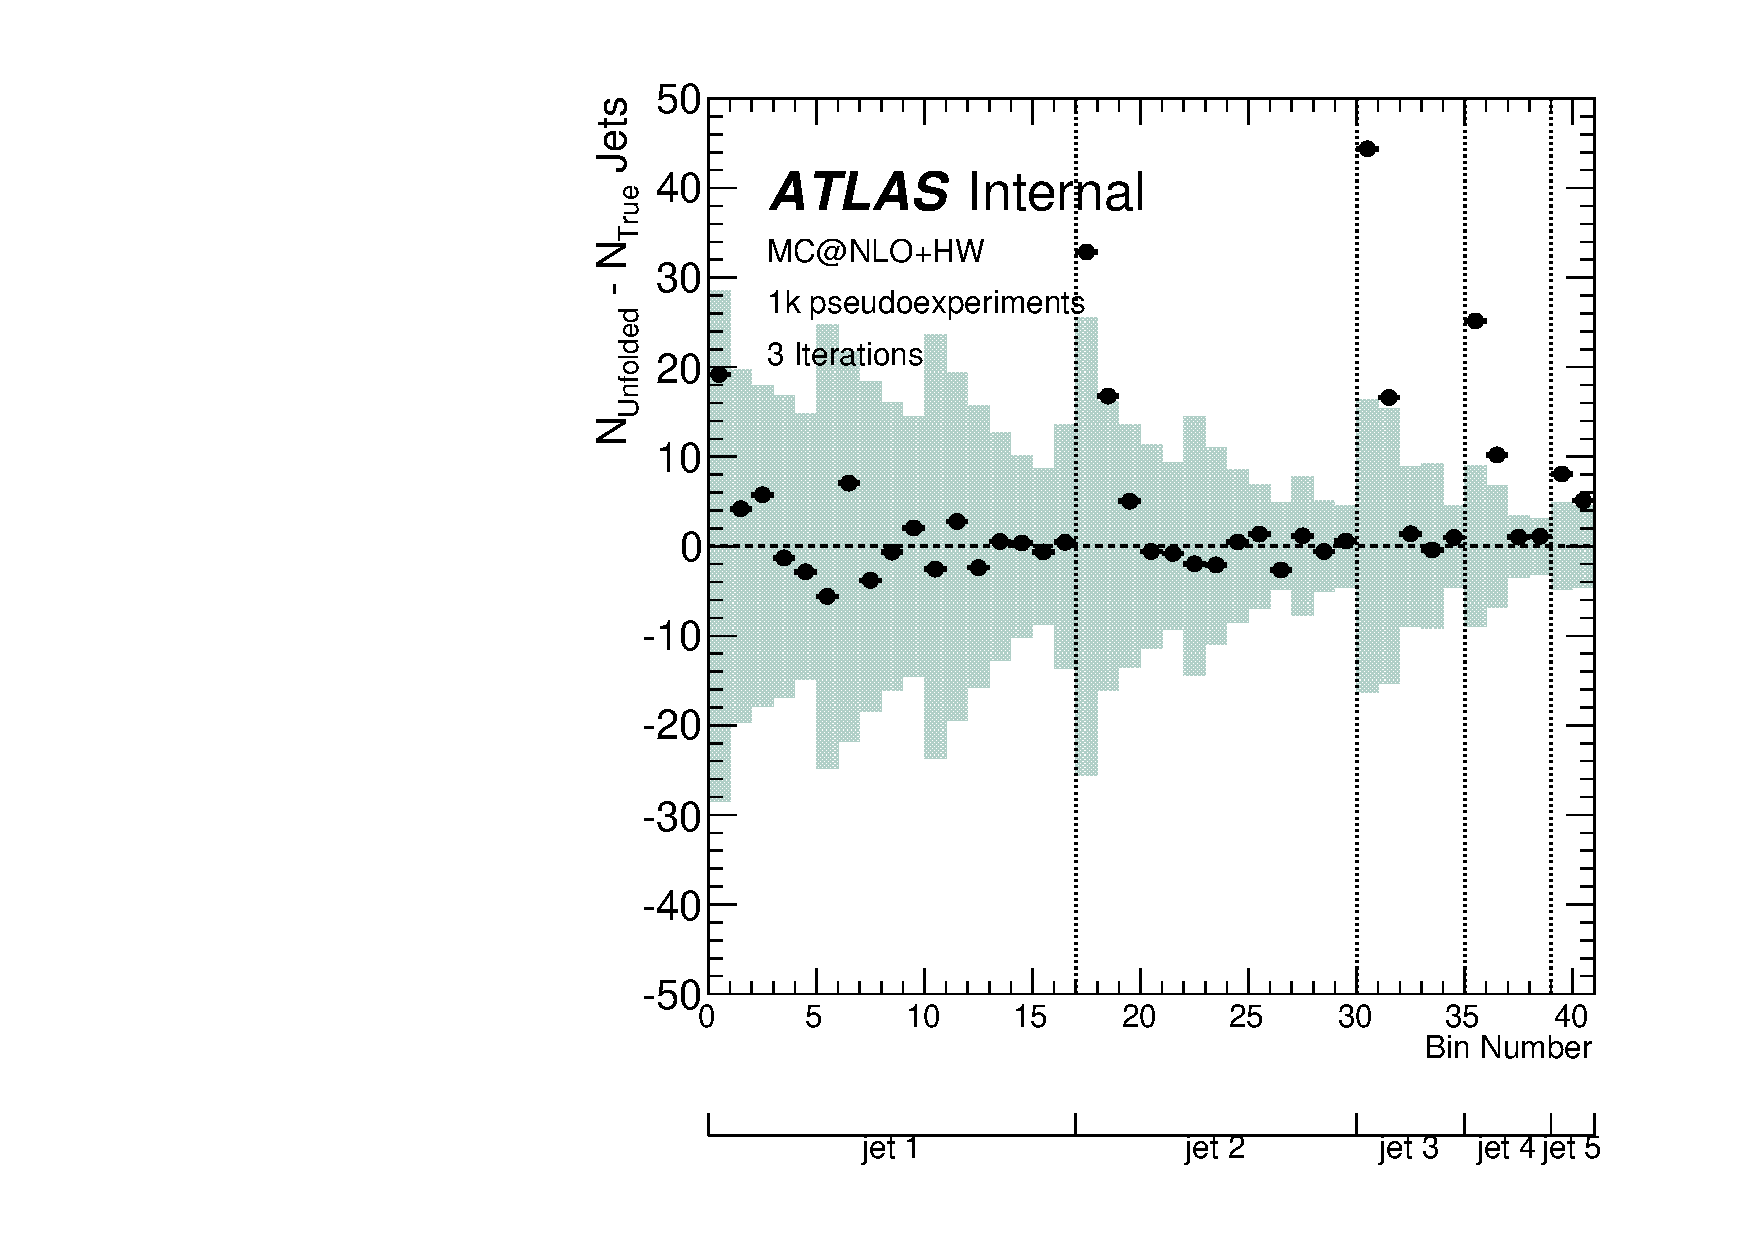
\includegraphics[width=\textwidth]{fig/Stress/105200atlfast/Bias3Iterations.pdf}
\end{subfigure}
\begin{subfigure}[]{0.5\textwidth}
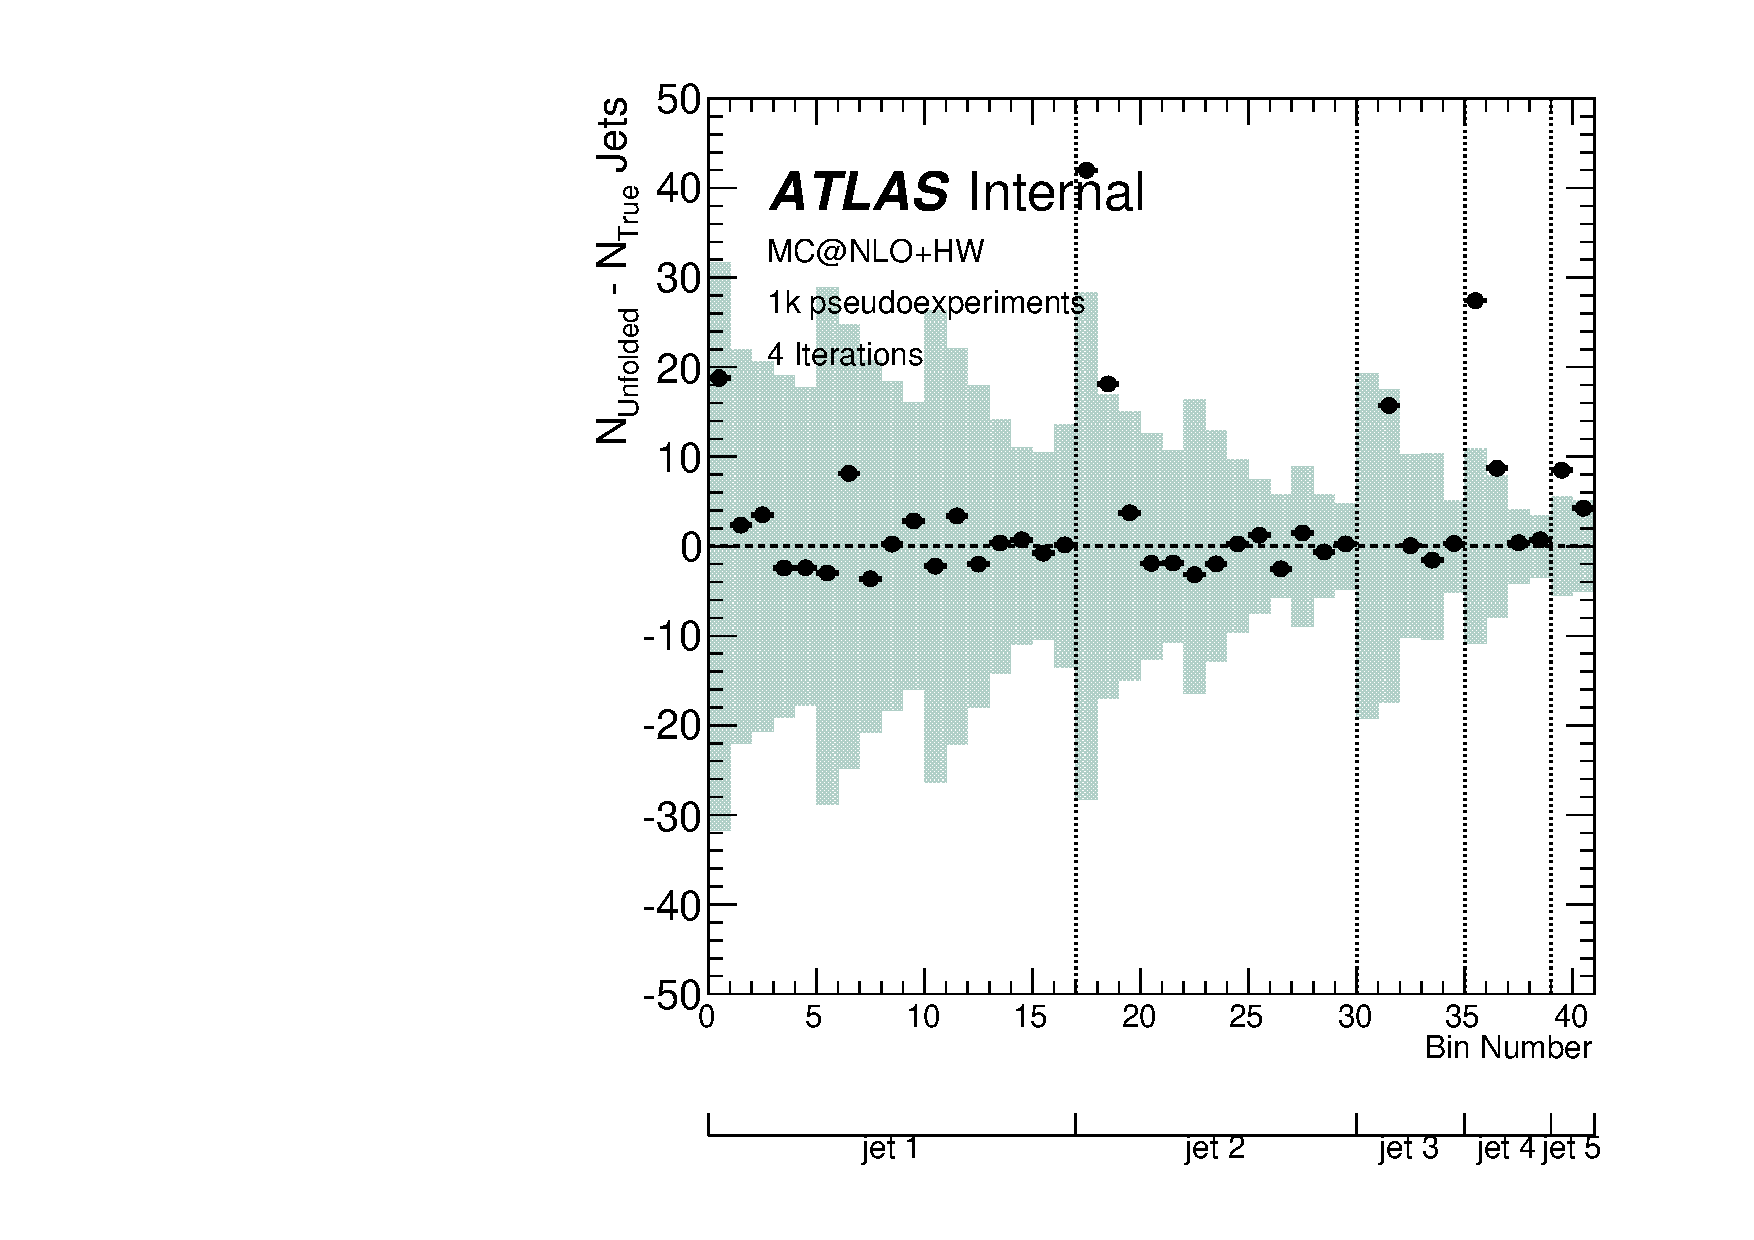
\includegraphics[width=\textwidth]{fig/Stress/105200atlfast/Bias4Iterations.pdf}
\end{subfigure}
\caption{Bias distribution for pseudoexperiments constructed from \newline \mcnlohw\ simulation unfolded against a matrix filled with the baseline simulation. One thousand pseudoexperiments, each the size of the events in data, are selected from the sample and unfolded. The Bayesian unfolding method with various numbers of iterations is used. Each bin of the distribution over the pseudoexperiments is fit with a gaussian. The black points show the fitted mean of each bin and the blue band shows the fitted sigma. }
\label{fig:mcnlohwbias}
\end{figure}
\clearpage
%\section{Pull \mcnlohw}
\begin{figure}
\begin{subfigure}[]{0.5\textwidth}
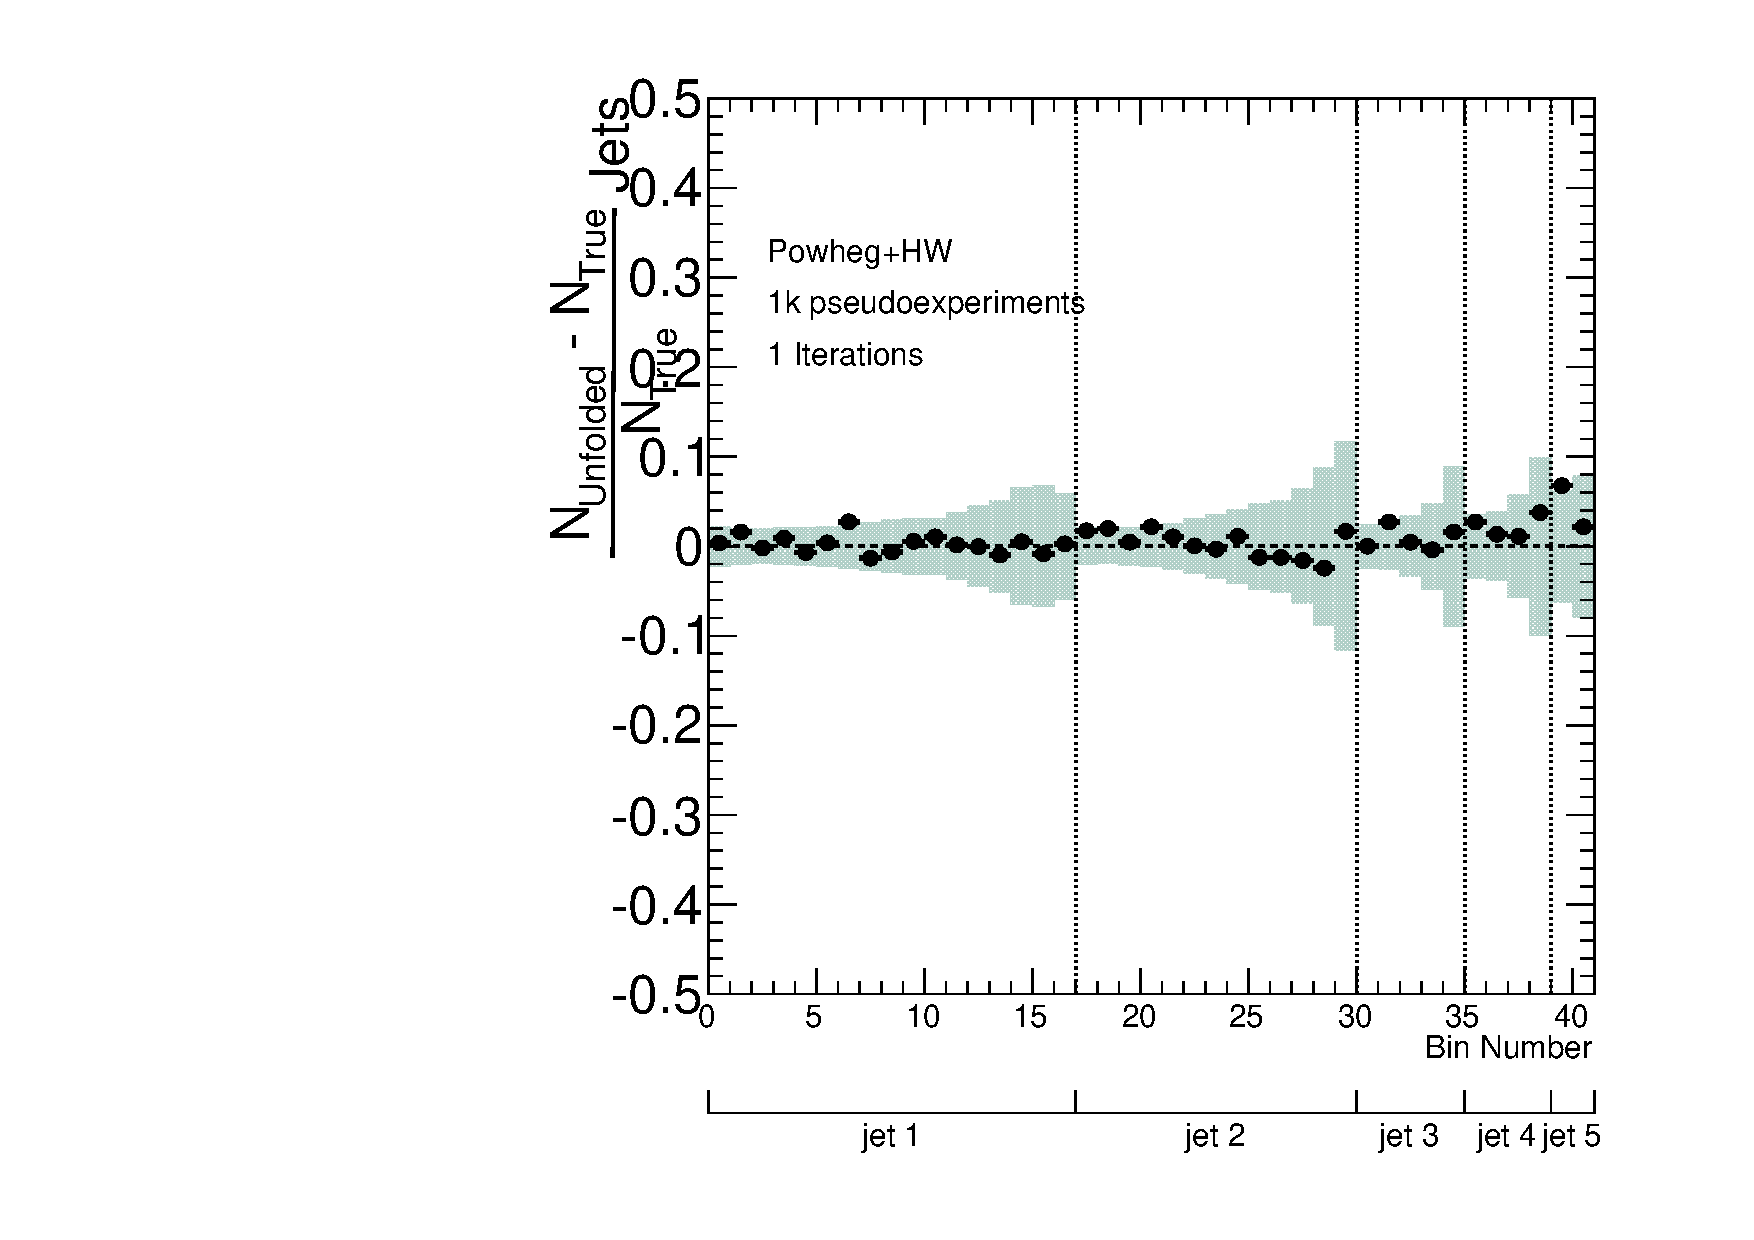
\includegraphics[width=\textwidth]{fig/Stress/105860atlfast/FracBias1Iterations.pdf}
\end{subfigure}
~
\begin{subfigure}[]{0.5\textwidth}
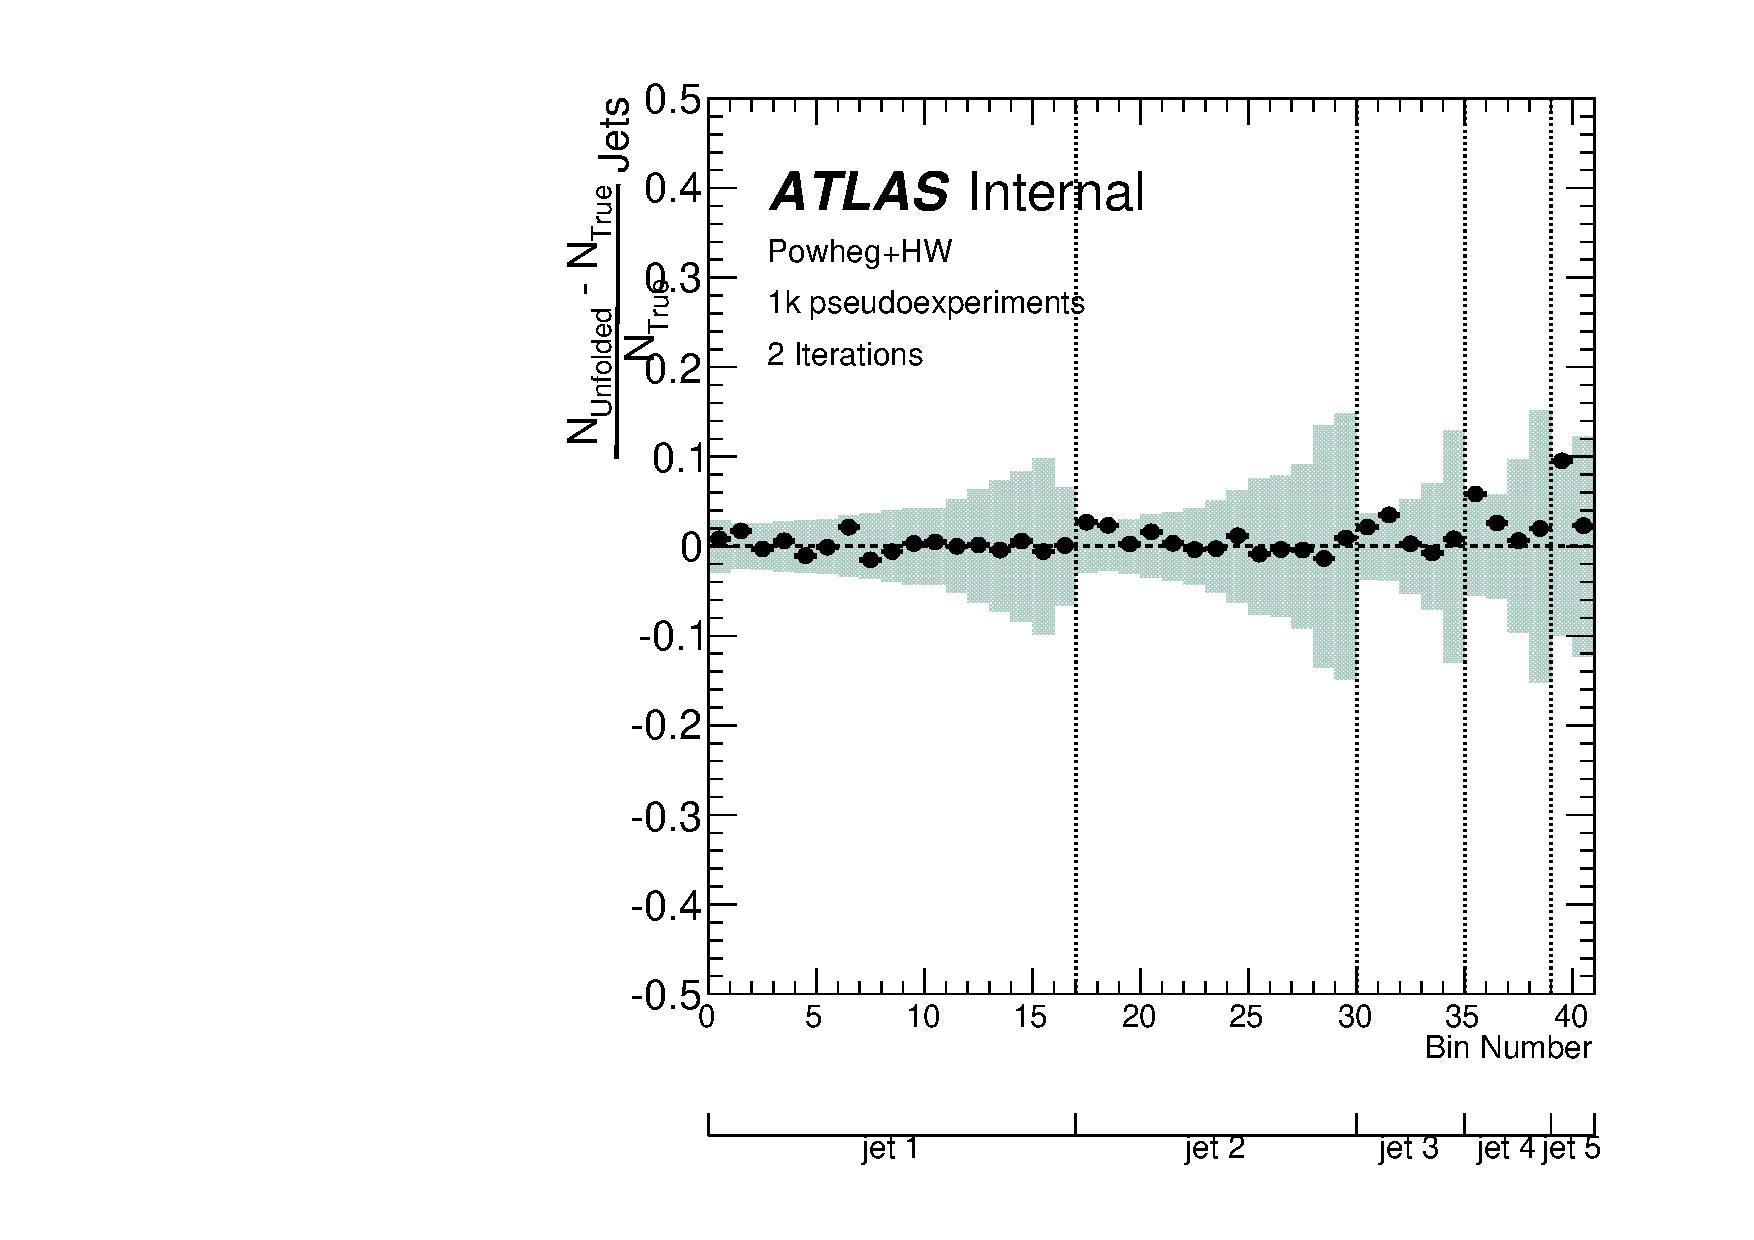
\includegraphics[width=\textwidth]{fig/Stress/105860atlfast/FracBias2Iterations.pdf}
\end{subfigure}
\\
\begin{subfigure}[]{0.5\textwidth}
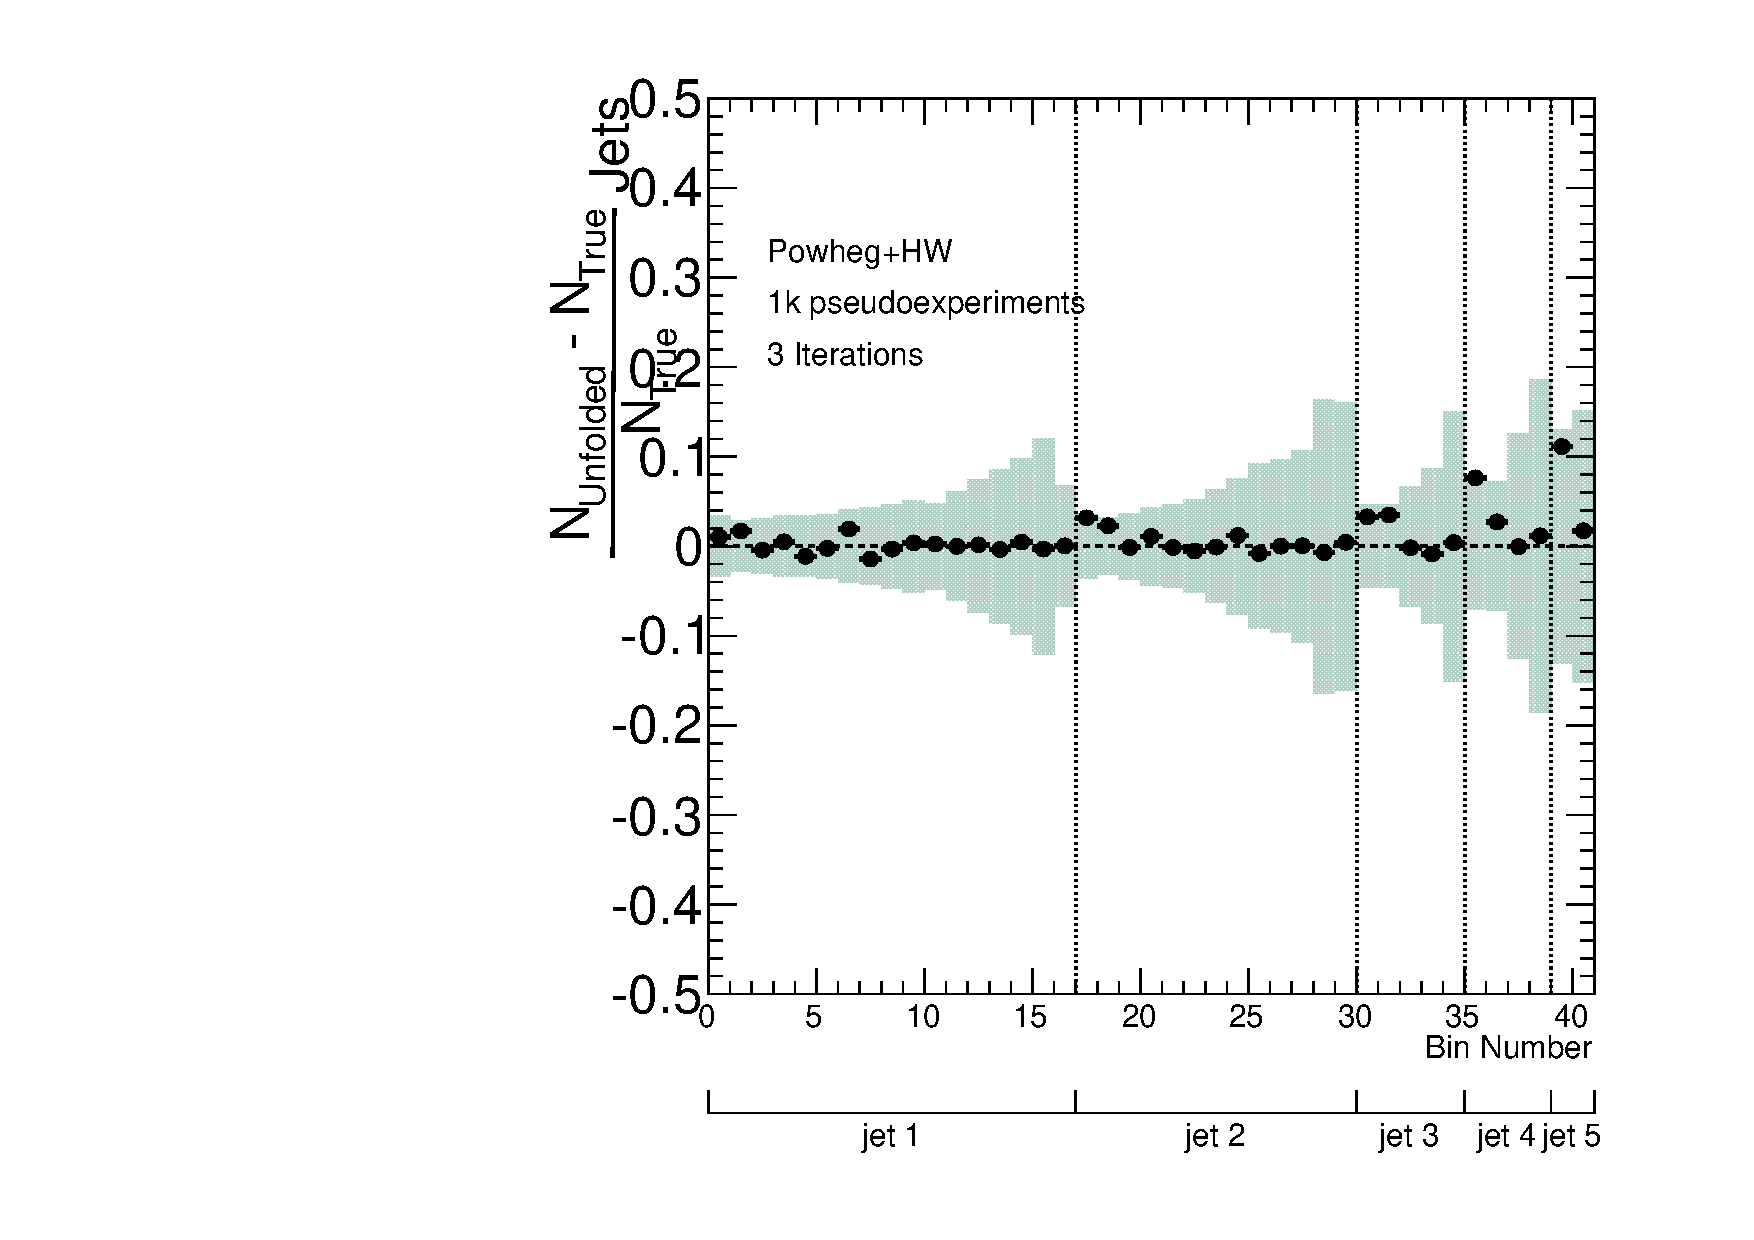
\includegraphics[width=\textwidth]{fig/Stress/105860atlfast/FracBias3Iterations.pdf}
\end{subfigure}
~
\begin{subfigure}[]{0.5\textwidth}
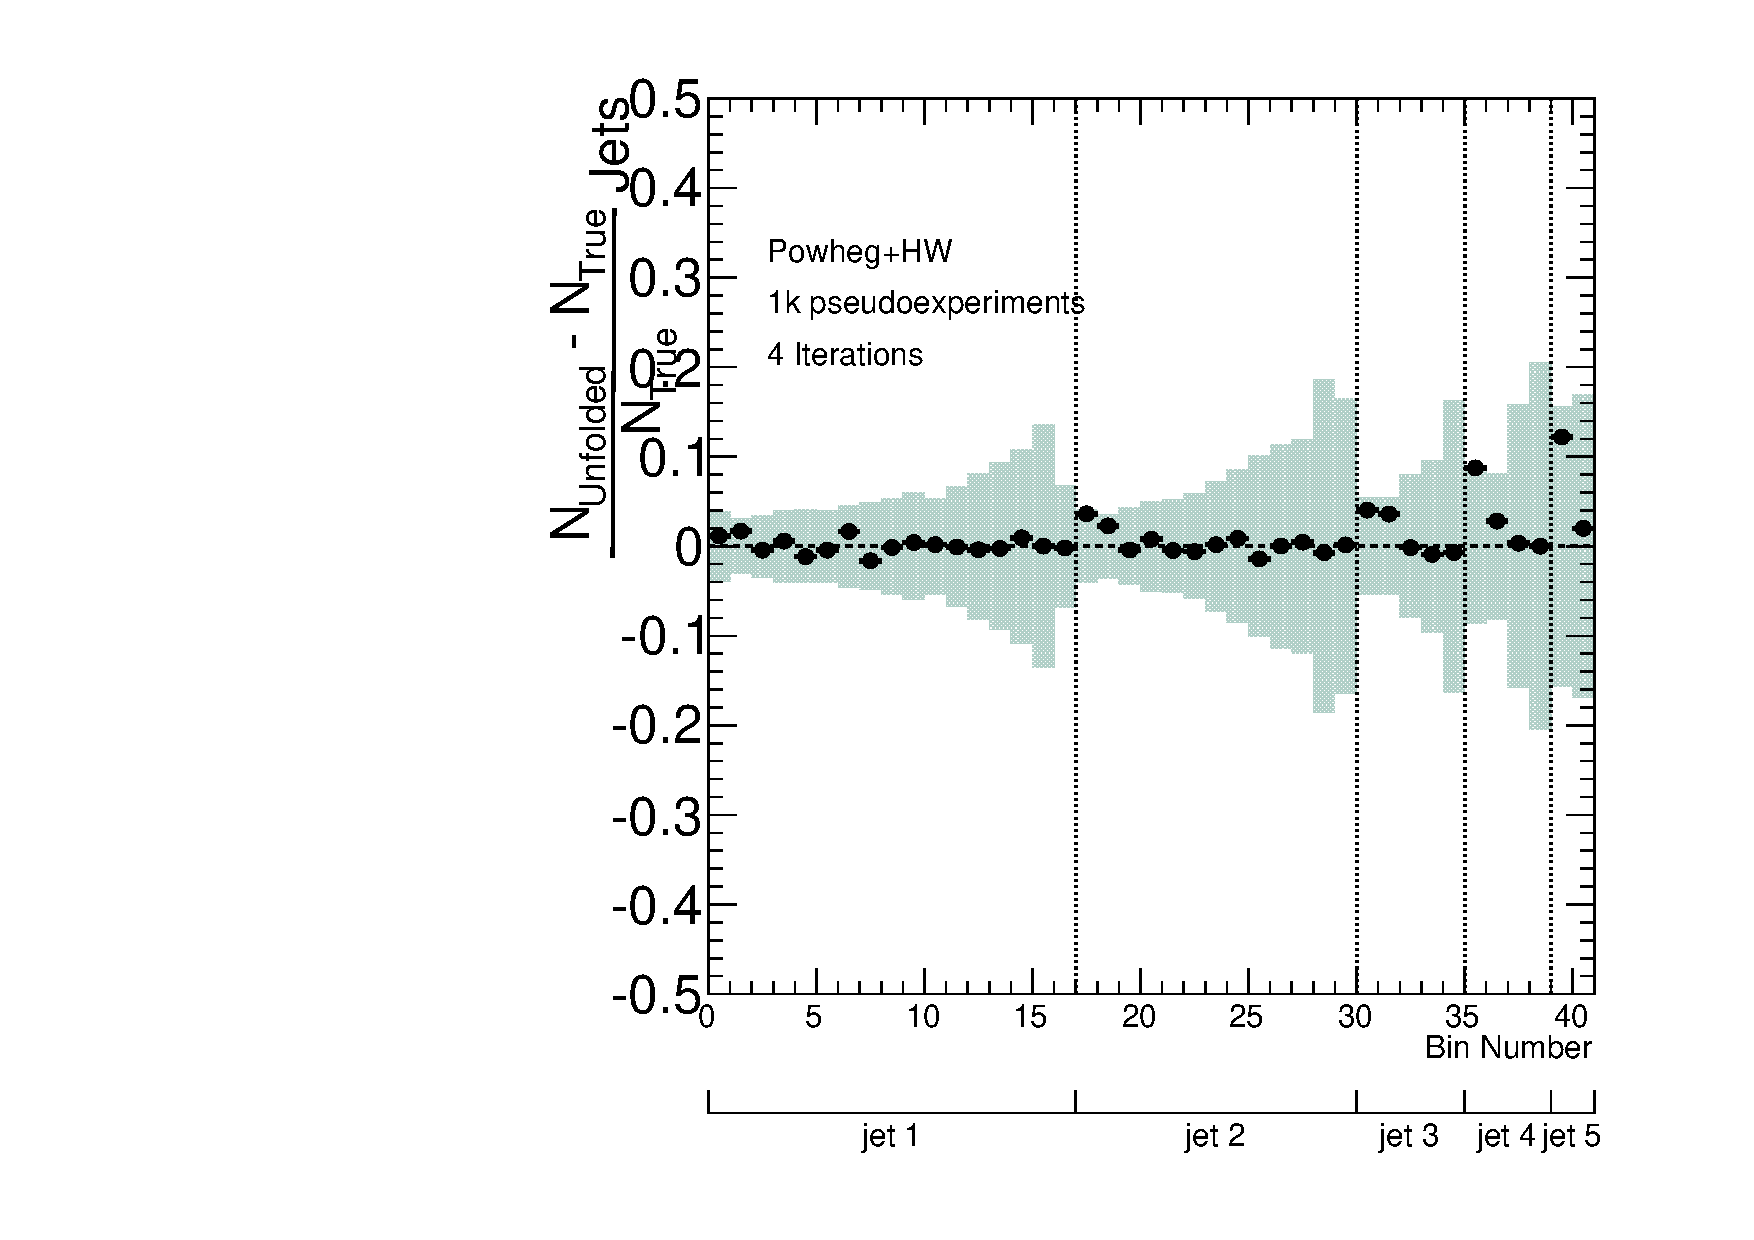
\includegraphics[width=\textwidth]{fig/Stress/105860atlfast/FracBias4Iterations.pdf}
\end{subfigure}
\caption{Fractional bias distribution for pseudoexperiments constructed from \newline \pow+\hw\ simulation unfolded against a matrix filled with the baseline simulation. One thousand pseudoexperiments, each the size of the events in data, are selected from the sample and unfolded. The Bayesian unfolding method with various numbers of iterations is used. Each bin of the distribution over the pseudoexperiments is fit with a gaussian. The black points show the fitted mean of each bin and the blue band shows the fitted sigma. }
\label{fig:powhwfrbias}
\end{figure}
\clearpage


%\section{Bias \hdamp}
\begin{figure}
\begin{subfigure}[]{0.5\textwidth}
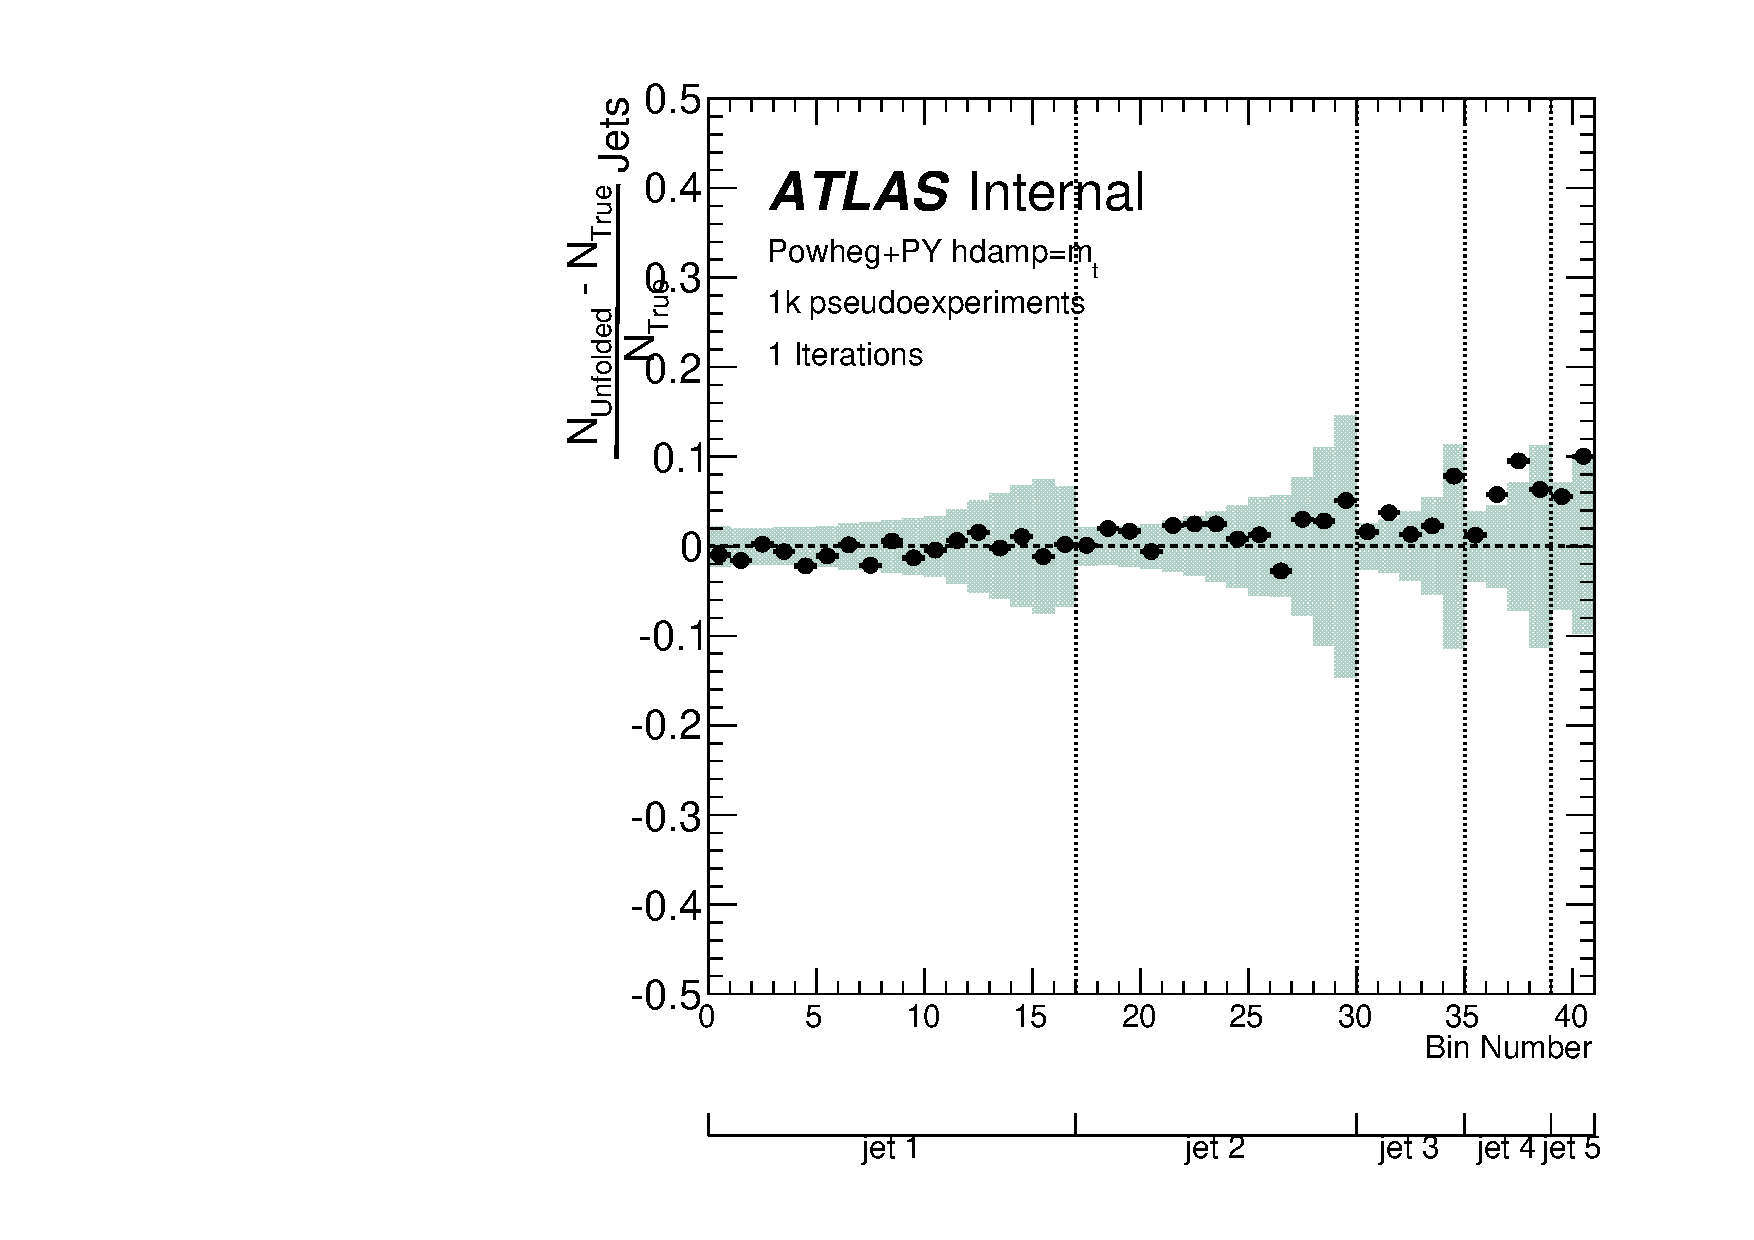
\includegraphics[width=\textwidth]{fig/Stress/110404atlfast/FracBias1Iterations.pdf}
\end{subfigure}
~
\begin{subfigure}[]{0.5\textwidth}
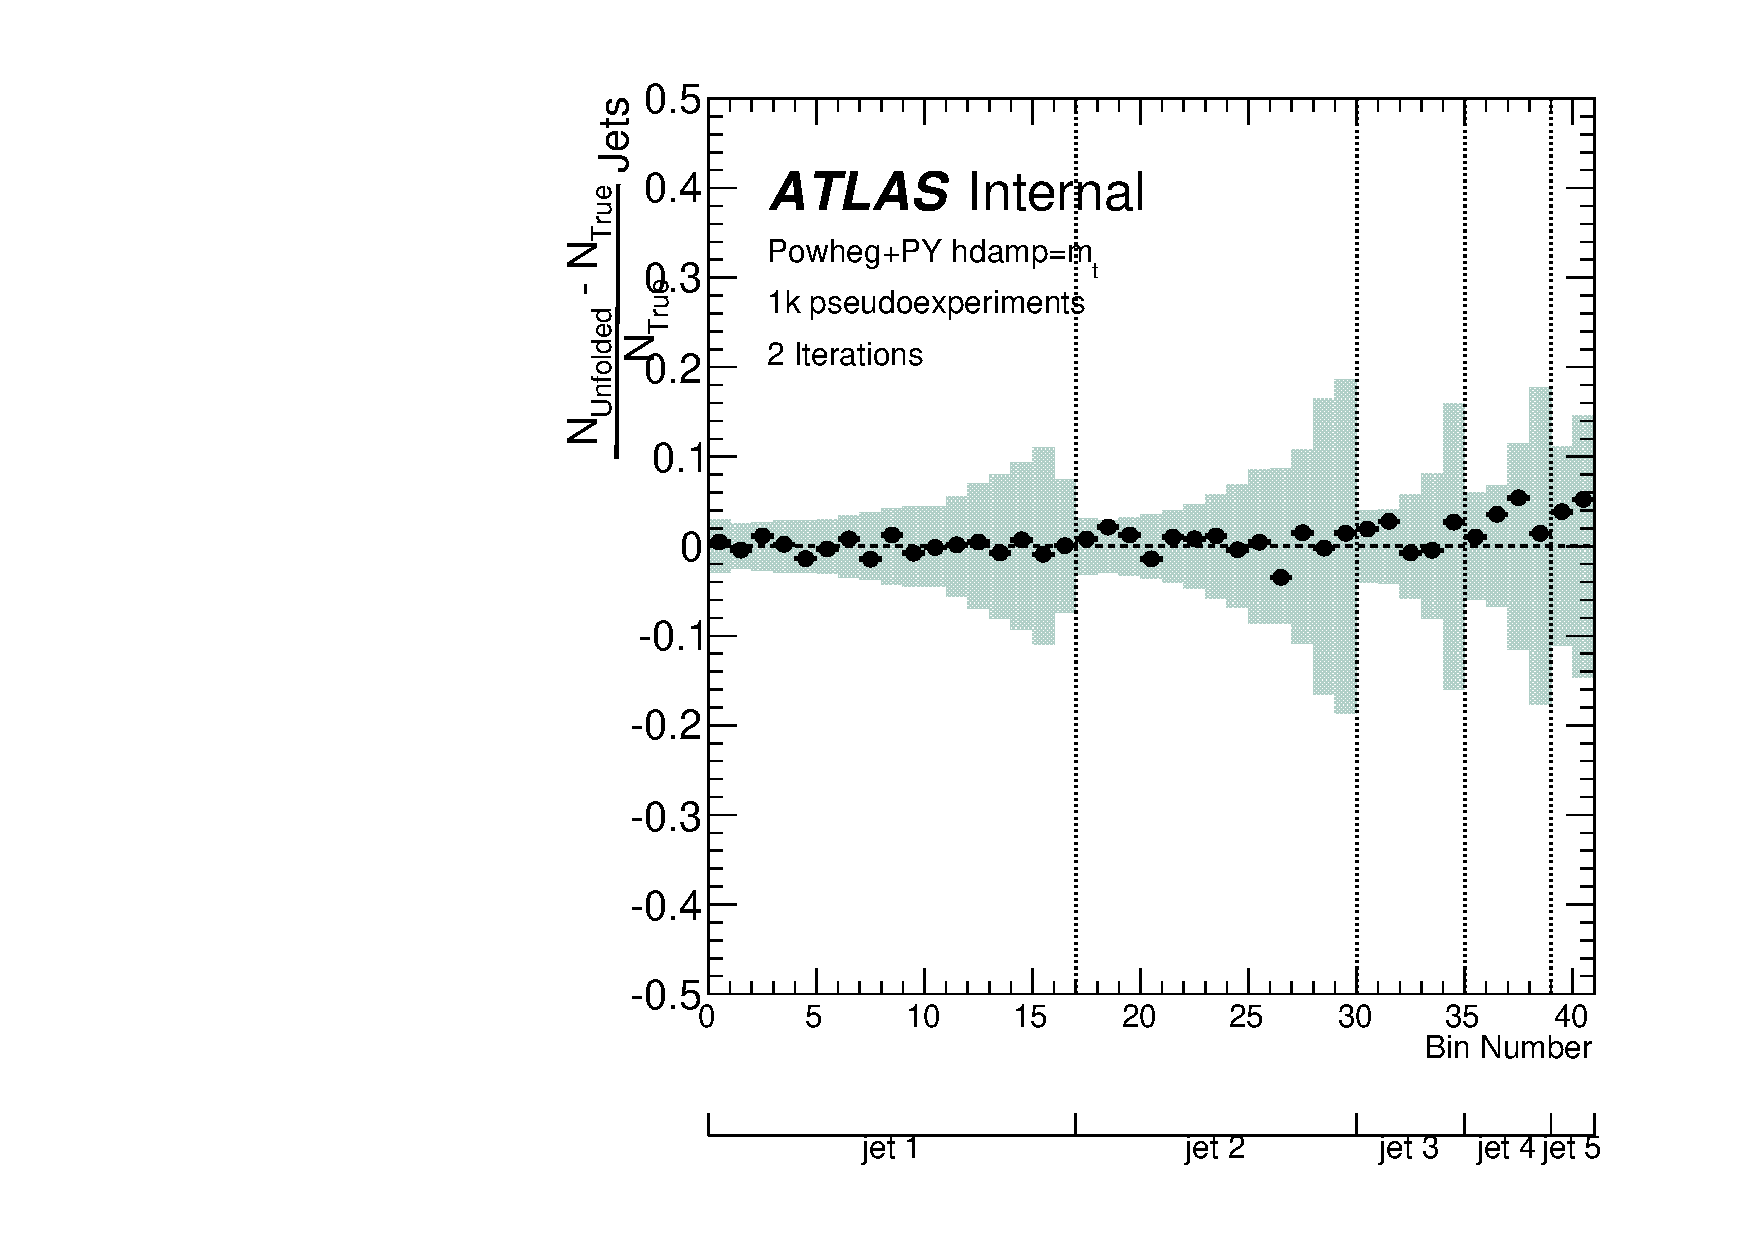
\includegraphics[width=\textwidth]{fig/Stress/110404atlfast/FracBias2Iterations.pdf}
\end{subfigure}
\\
\begin{subfigure}[]{0.5\textwidth}
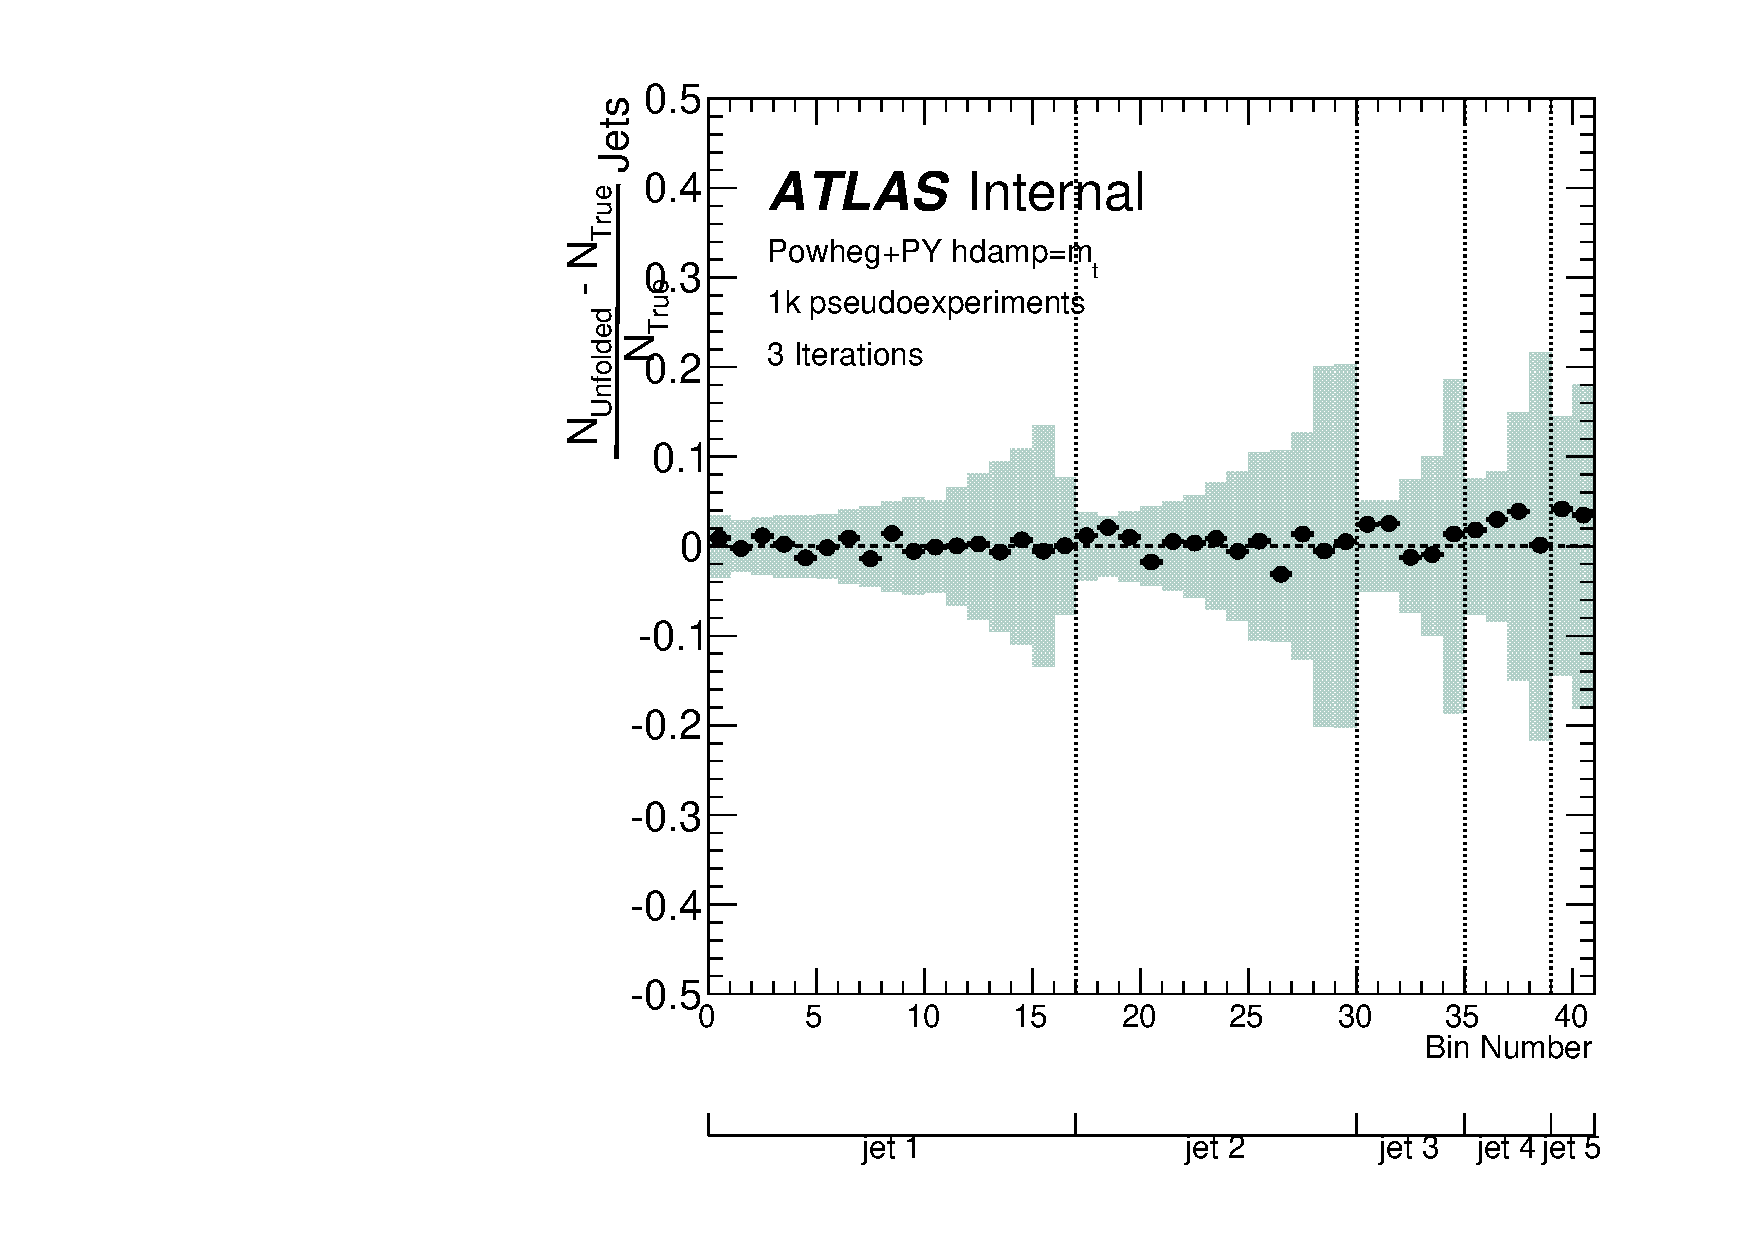
\includegraphics[width=\textwidth]{fig/Stress/110404atlfast/FracBias3Iterations.pdf}
\end{subfigure}
~
\begin{subfigure}[]{0.5\textwidth}
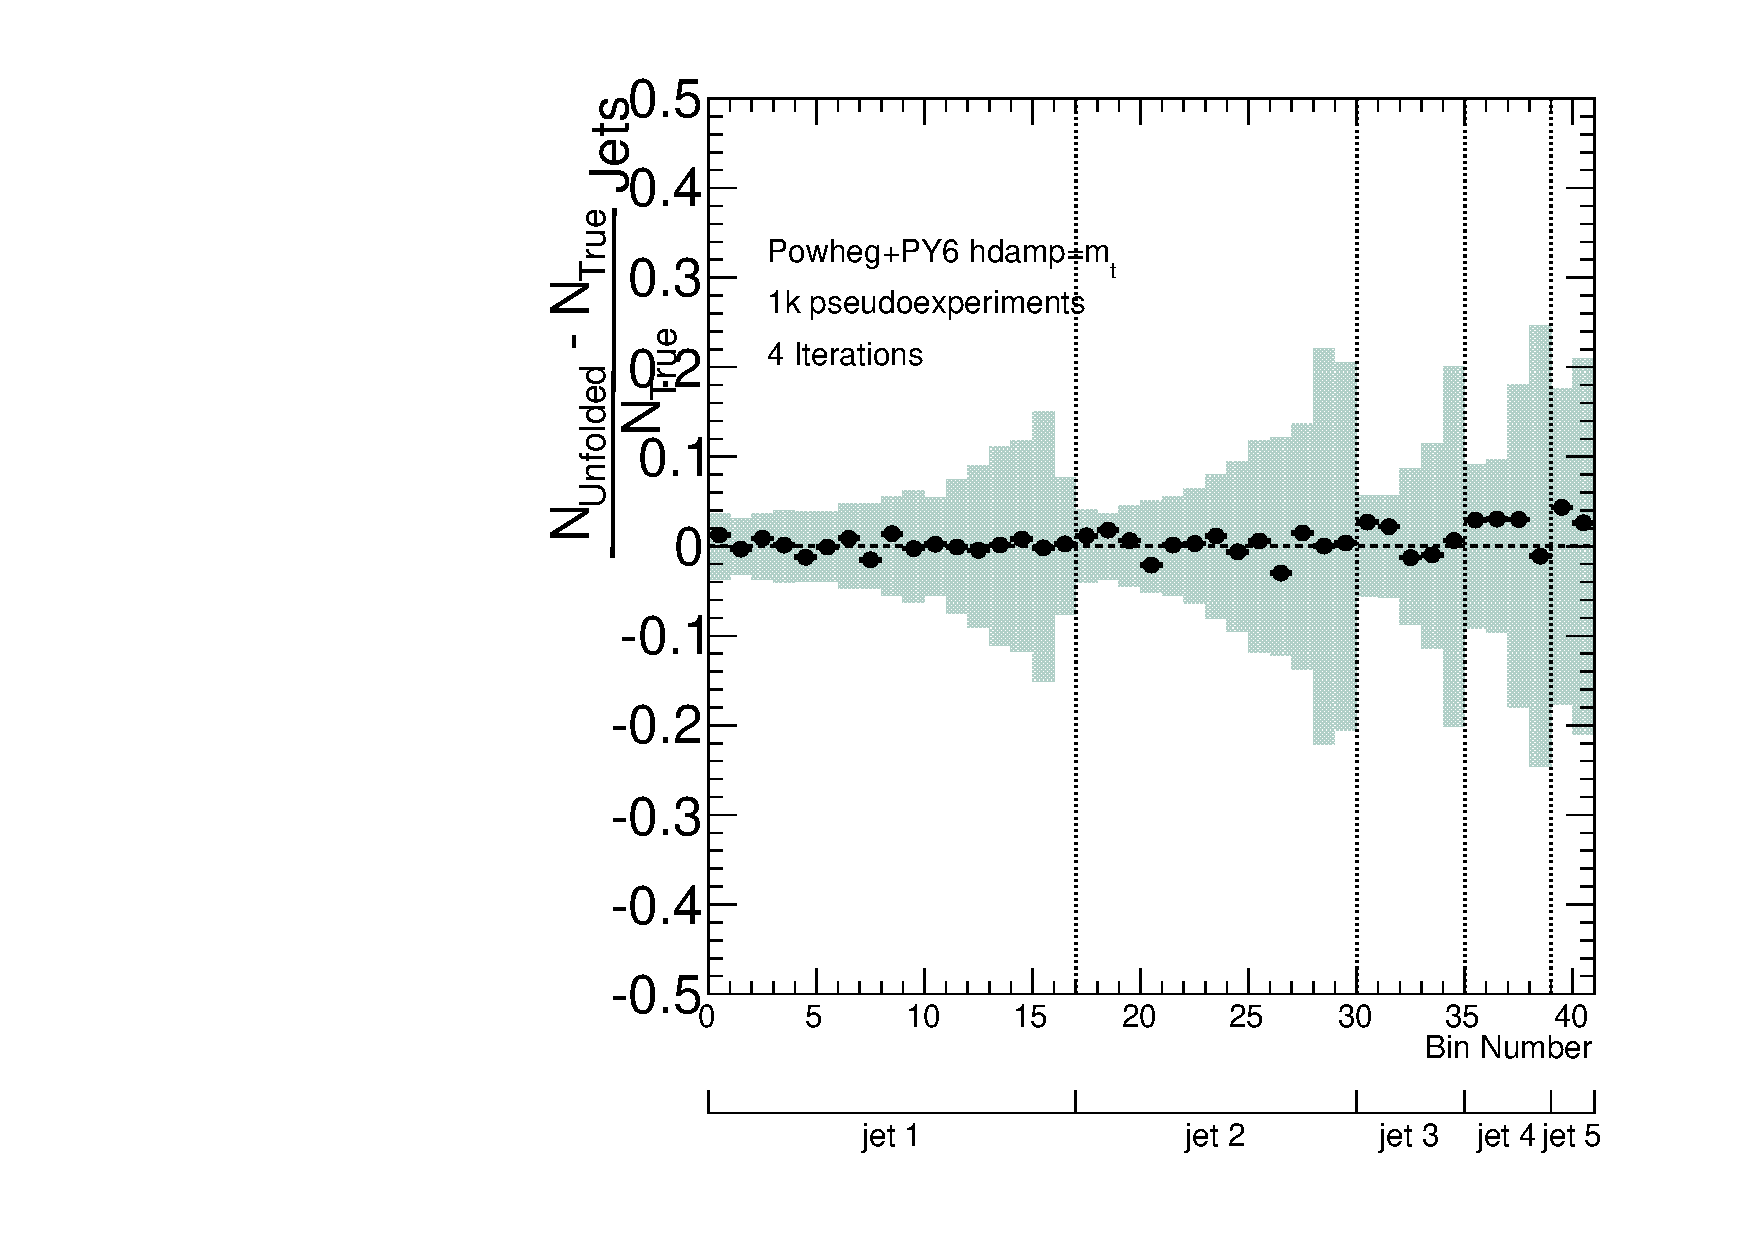
\includegraphics[width=\textwidth]{fig/Stress/110404atlfast/FracBias4Iterations.pdf}
\end{subfigure}
\caption{Fractional bias distribution for pseudoexperiments constructed from \newline \hdamp~ simulation unfolded against a matrix filled with the baseline simulation. One thousand pseudoexperiments, each the size of the events in data, are selected from the sample and unfolded. The Bayesian unfolding method with various numbers of iterations is used. Each bin of the distribution over the pseudoexperiments is fit with a gaussian. The black points show the fitted mean of each bin and the blue band shows the fitted sigma. }
\label{fig:hdampfrbias}
\end{figure}
\clearpage
%\section{Bias \peight}
\begin{figure}
\begin{subfigure}[]{0.5\textwidth}
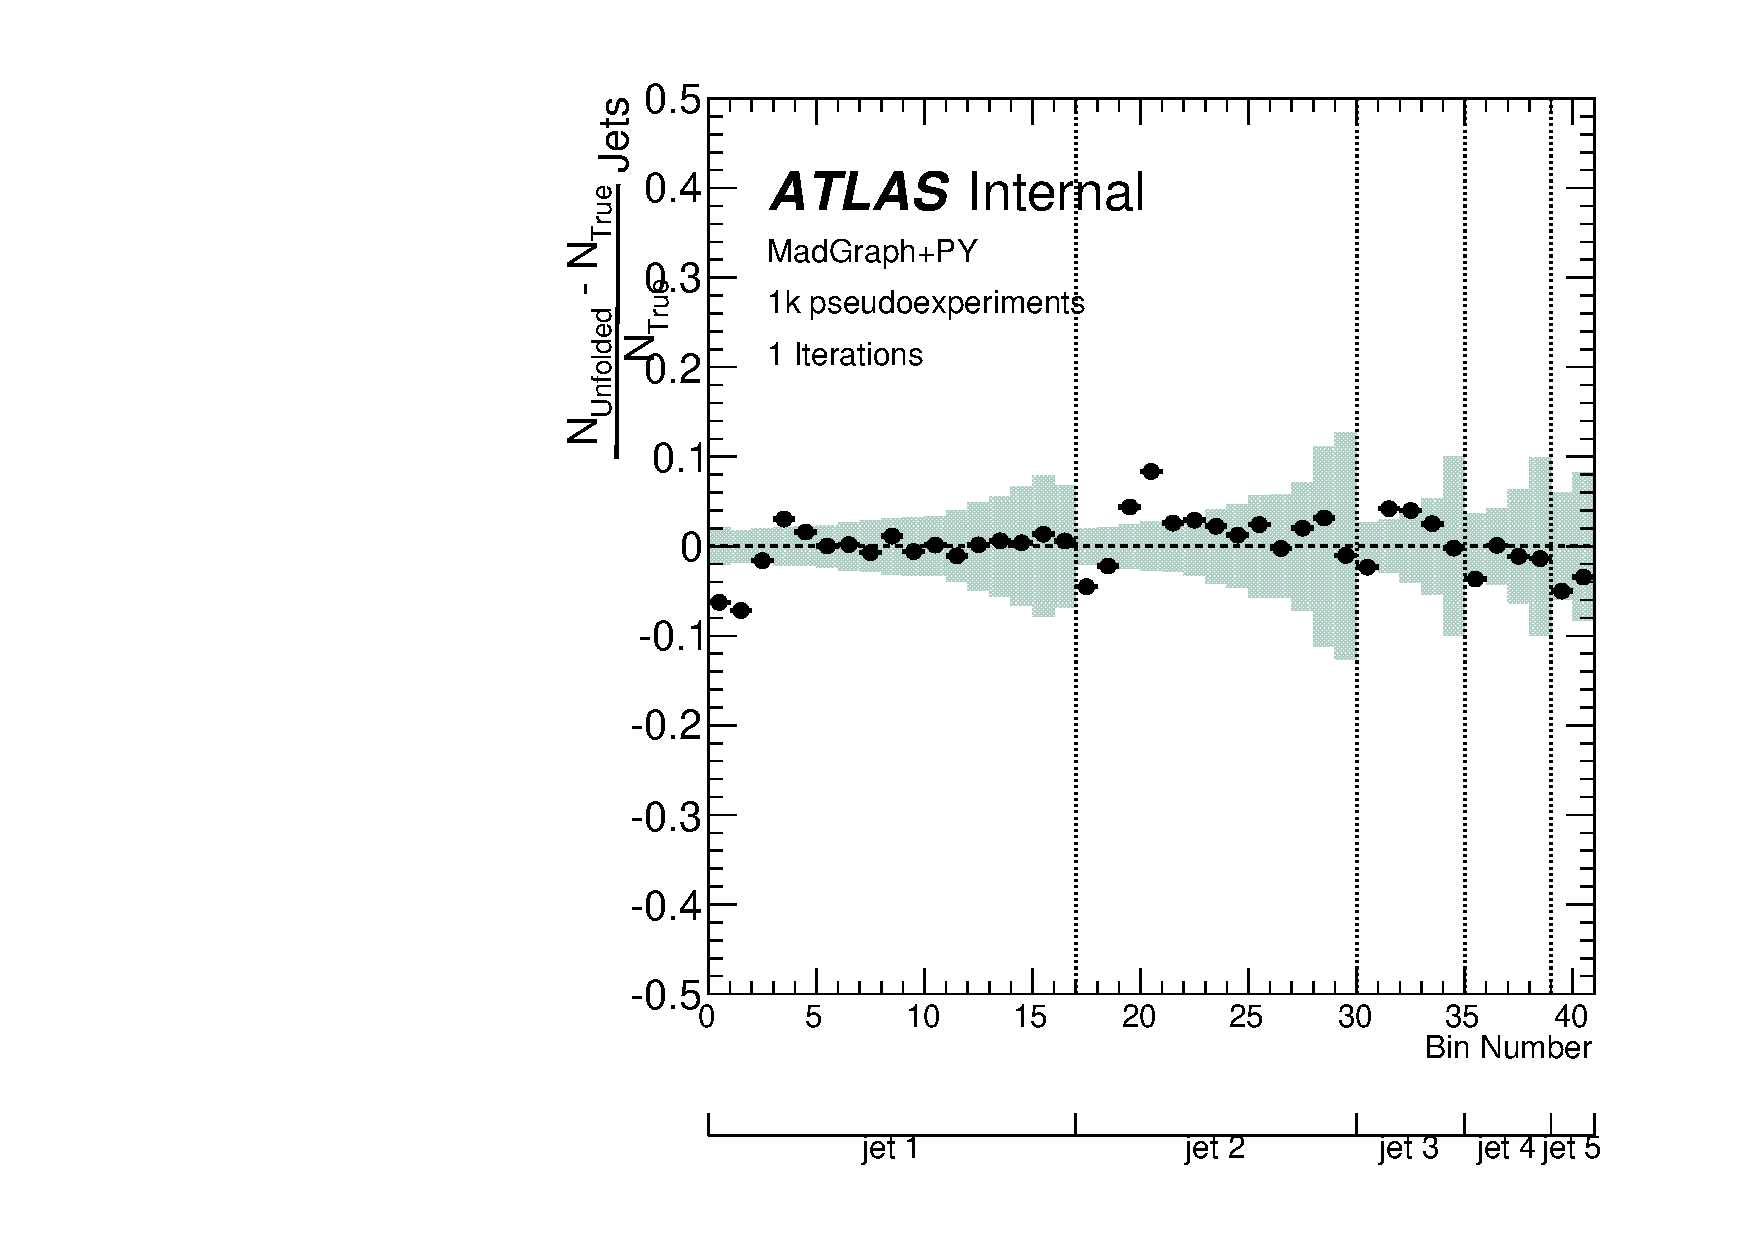
\includegraphics[width=\textwidth]{fig/Stress/110872atlfast/FracBias1Iterations.pdf}
\end{subfigure}
~
\begin{subfigure}[]{0.5\textwidth}
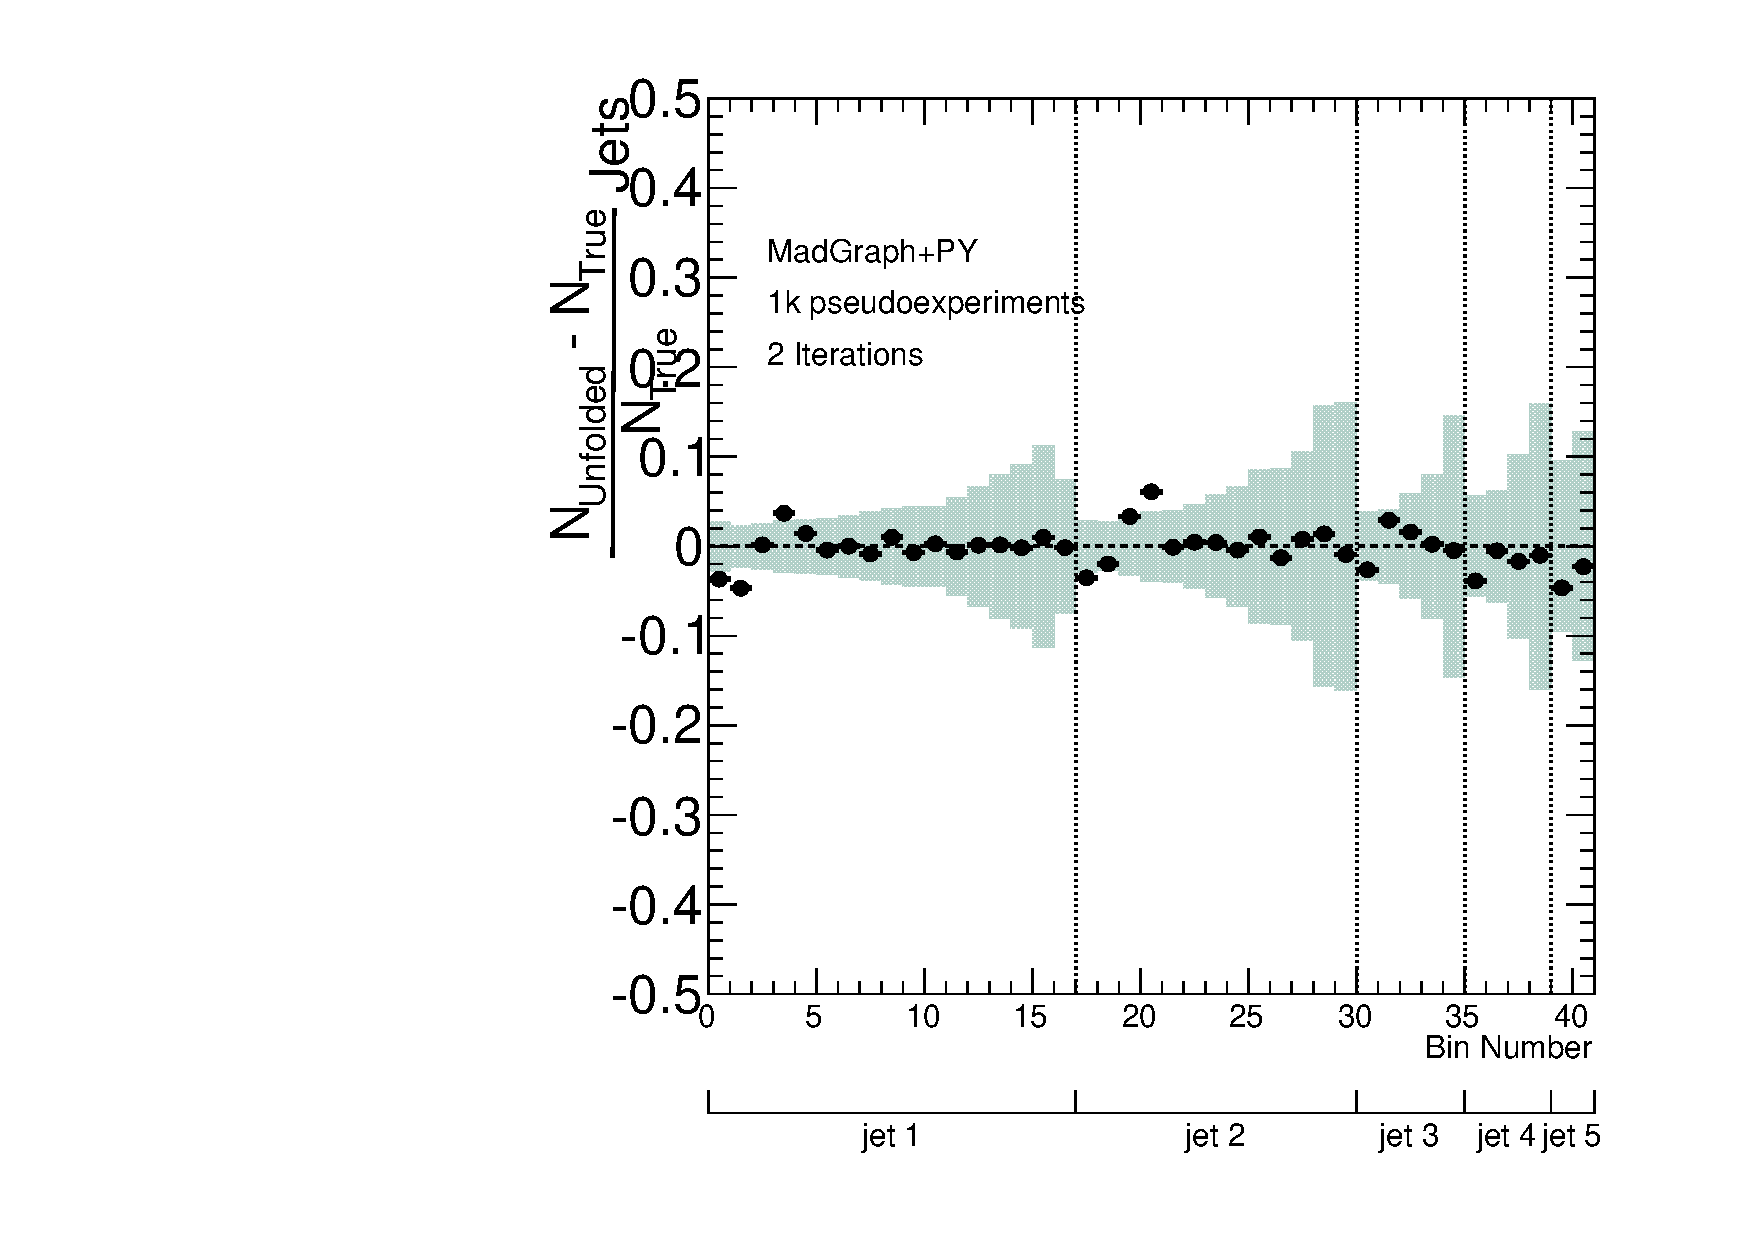
\includegraphics[width=\textwidth]{fig/Stress/110872atlfast/FracBias2Iterations.pdf}
\end{subfigure}
\\
\begin{subfigure}[]{0.5\textwidth}
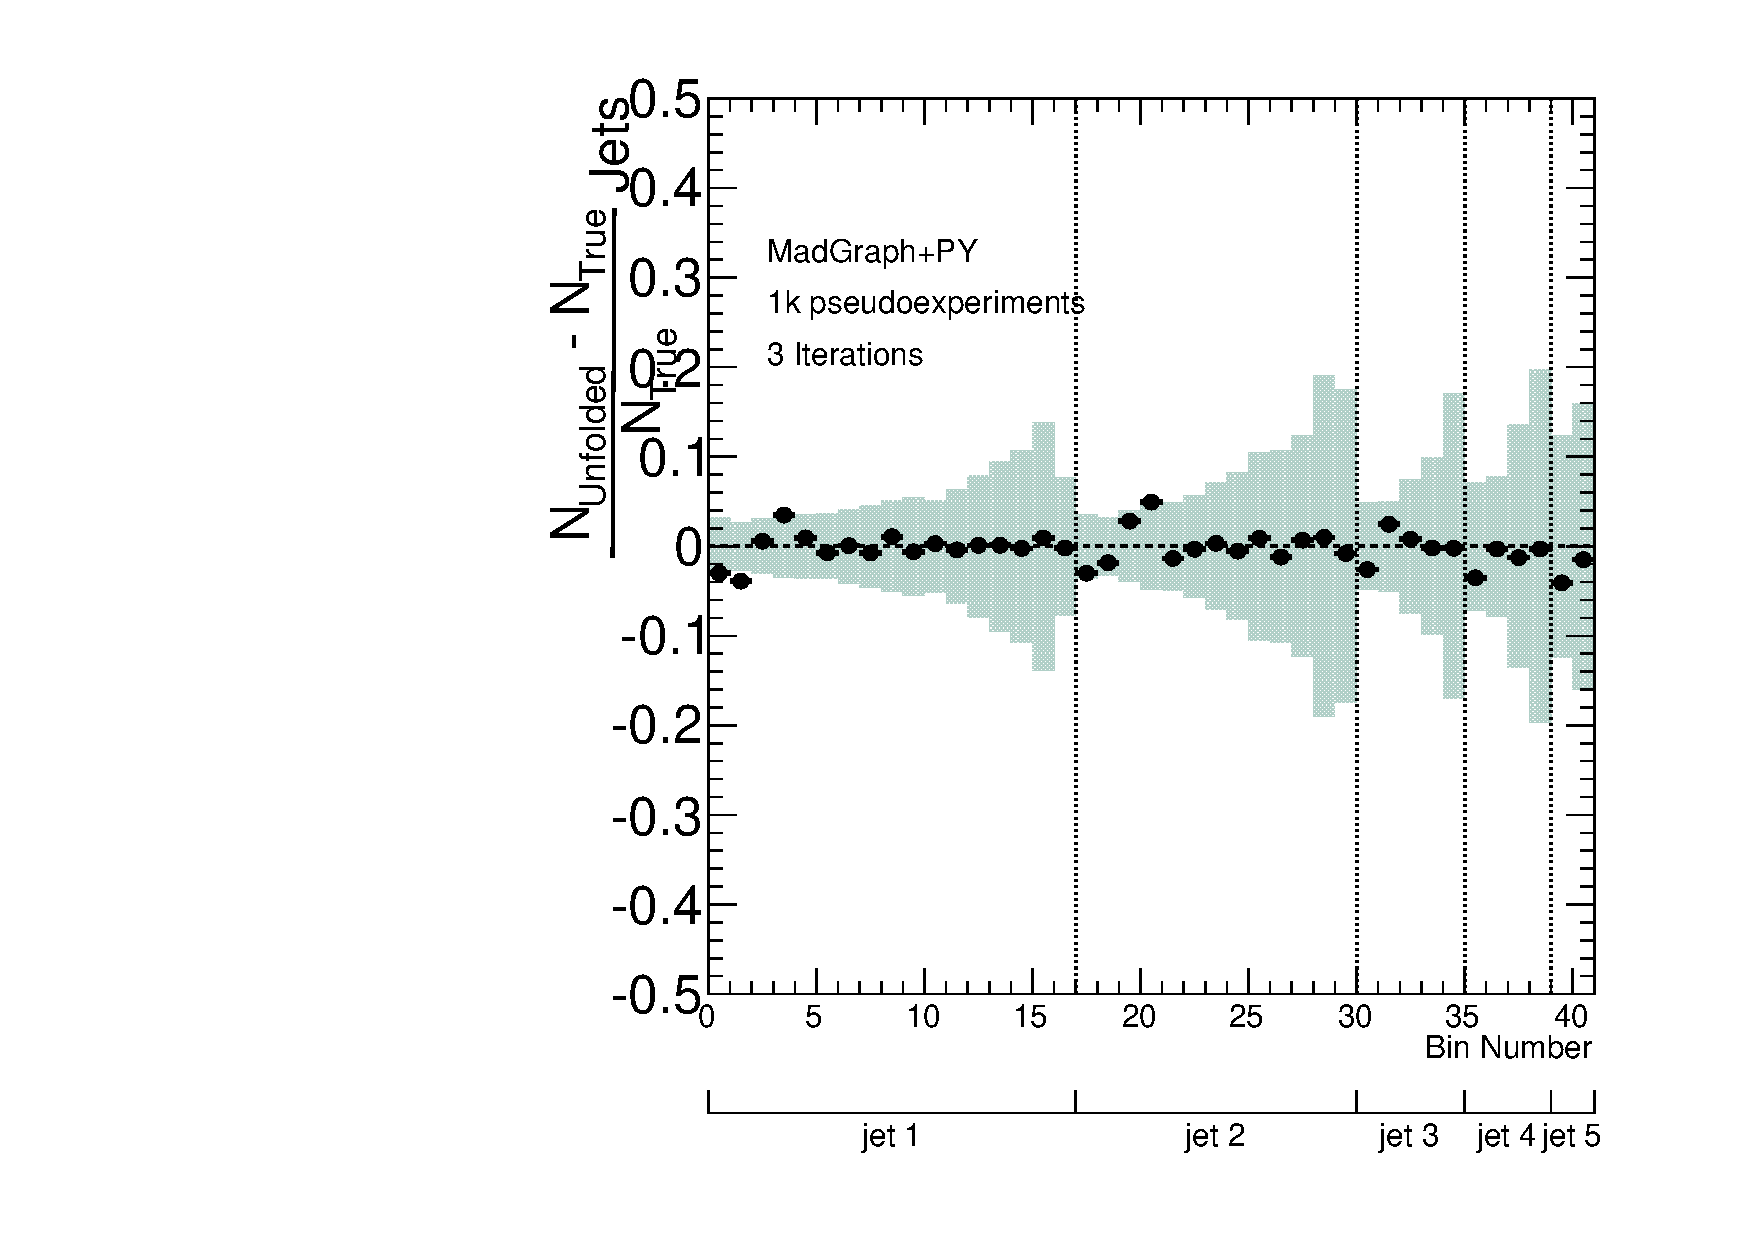
\includegraphics[width=\textwidth]{fig/Stress/110872atlfast/FracBias3Iterations.pdf}
\end{subfigure}
~
\begin{subfigure}[]{0.5\textwidth}
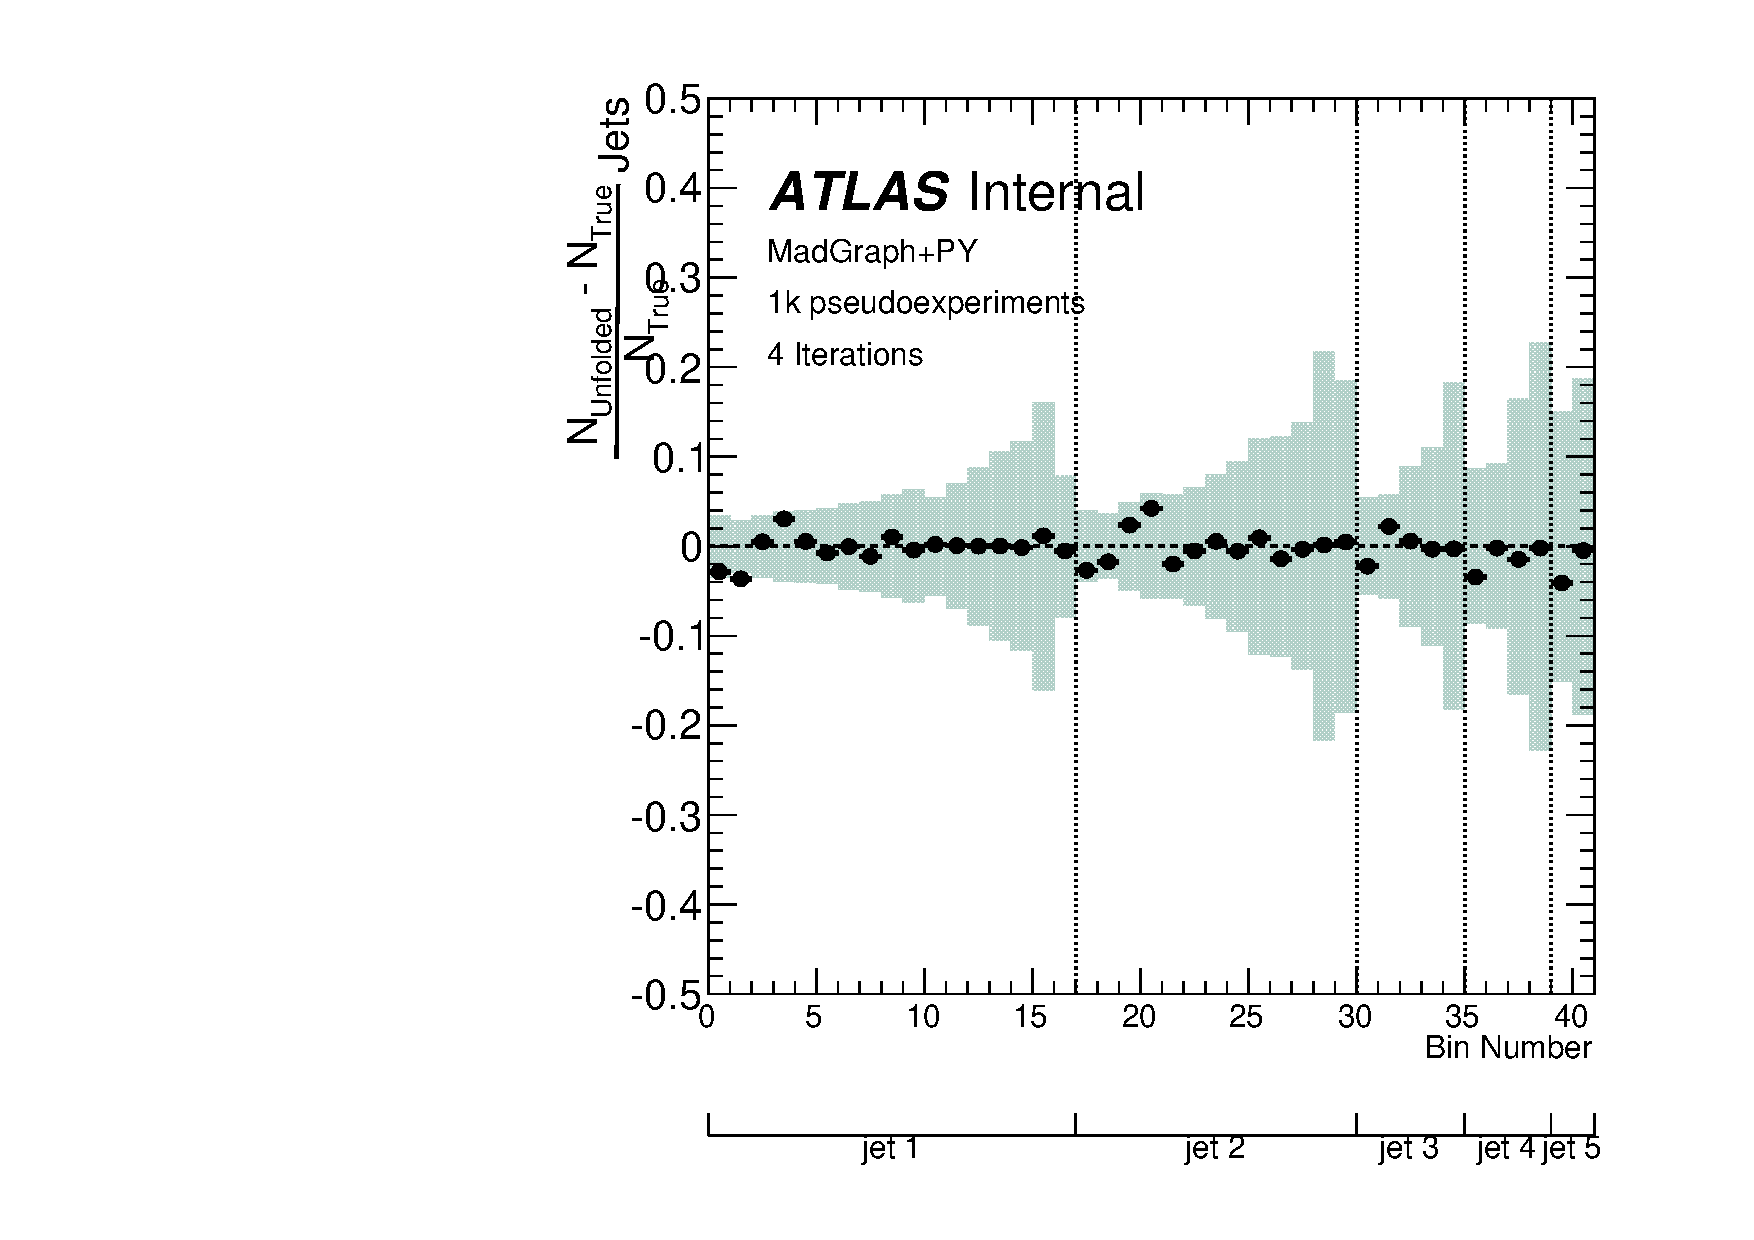
\includegraphics[width=\textwidth]{fig/Stress/110872atlfast/FracBias4Iterations.pdf}
\end{subfigure}
\caption{Fractional bias distribution for pseudoexperiments constructed from \newline \madpy\ simulation unfolded against a matrix filled with the baseline simulation. One thousand pseudoexperiments, each the size of the events in data, are selected from the sample and unfolded. The Bayesian unfolding method with various numbers of iterations is used. Each bin of the distribution over the pseudoexperiments is fit with a gaussian. The black points show the fitted mean of each bin and the blue band shows the fitted sigma.}
\label{fig:p8frbias}
\end{figure}
\clearpage
%\section{Bias \powpy\ fullsim}
\begin{figure}
\begin{subfigure}[]{0.5\textwidth}
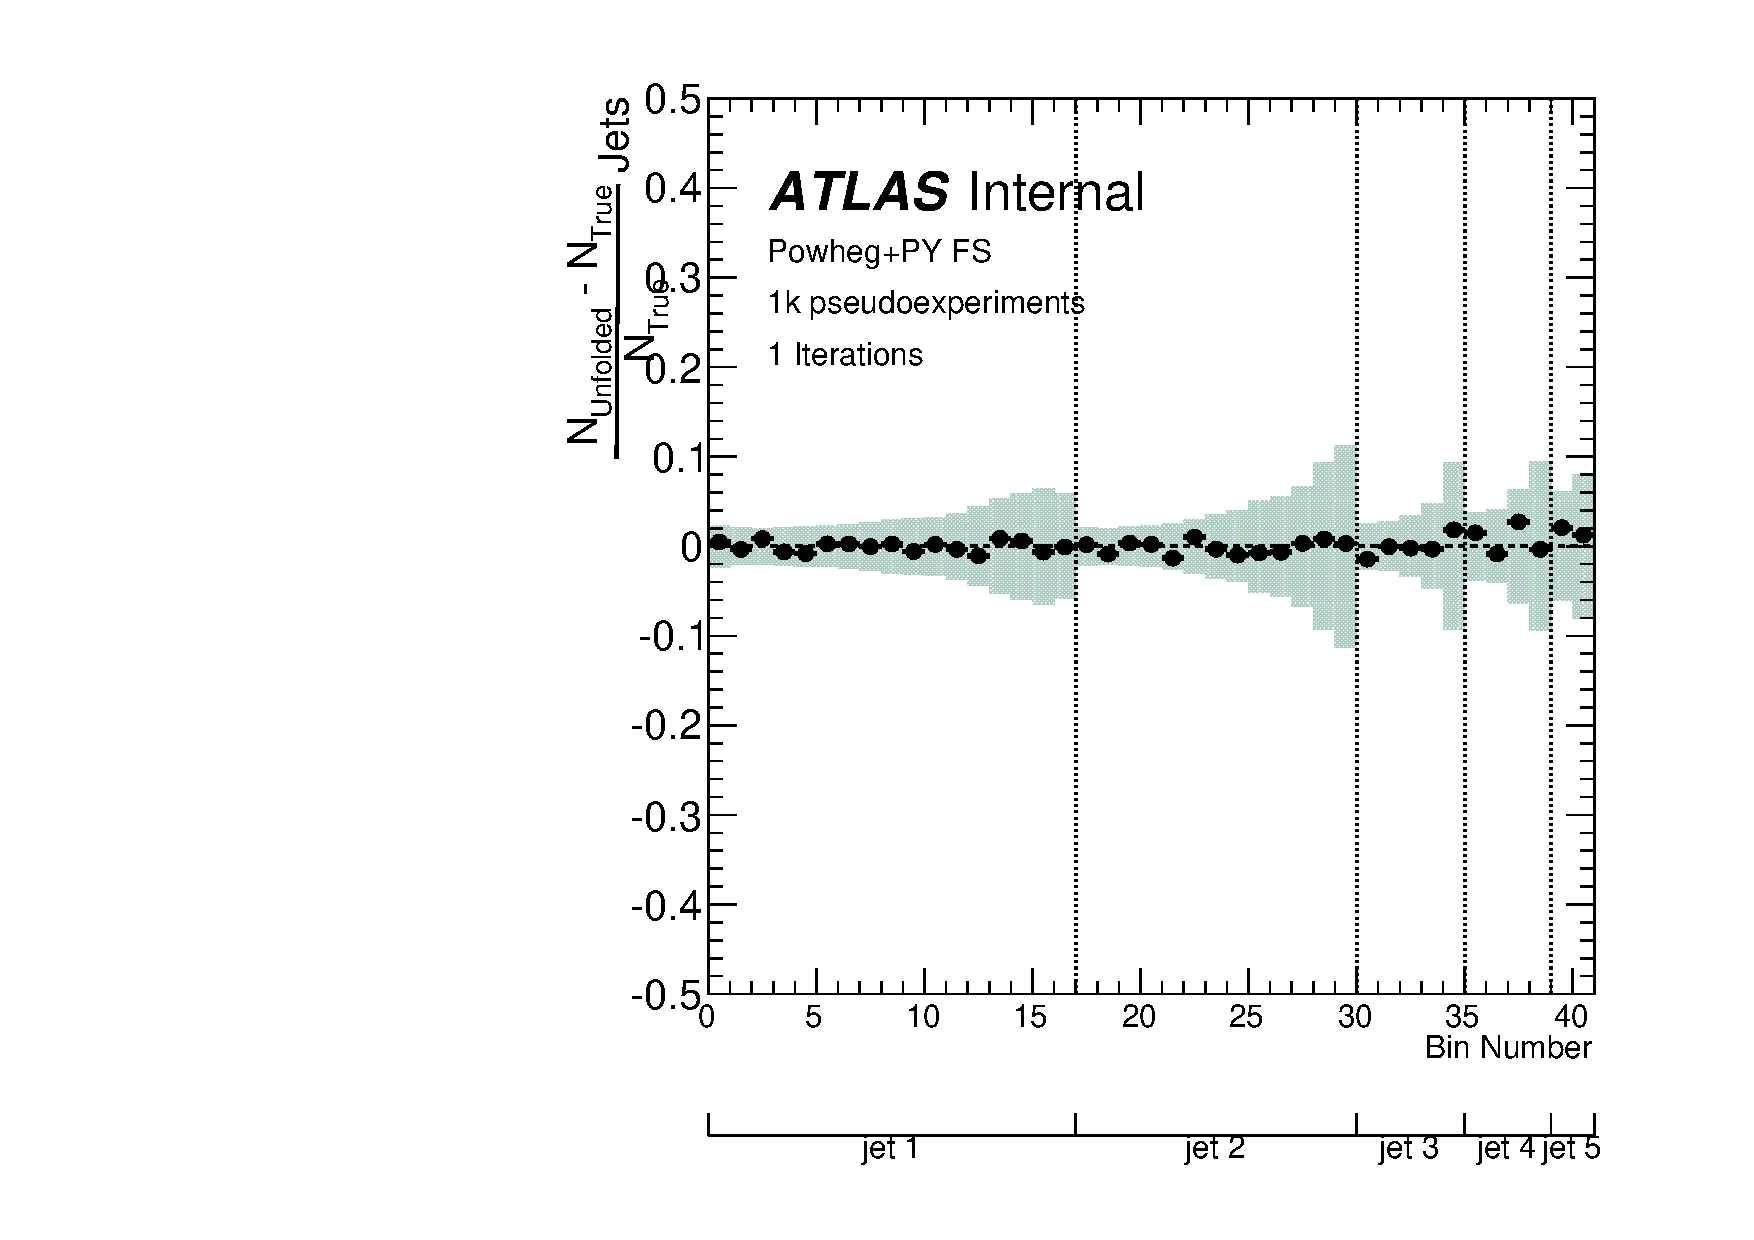
\includegraphics[width=\textwidth]{fig/Stress/117050fullsim/FracBias1Iterations.pdf}
\end{subfigure}
~
\begin{subfigure}[]{0.5\textwidth}
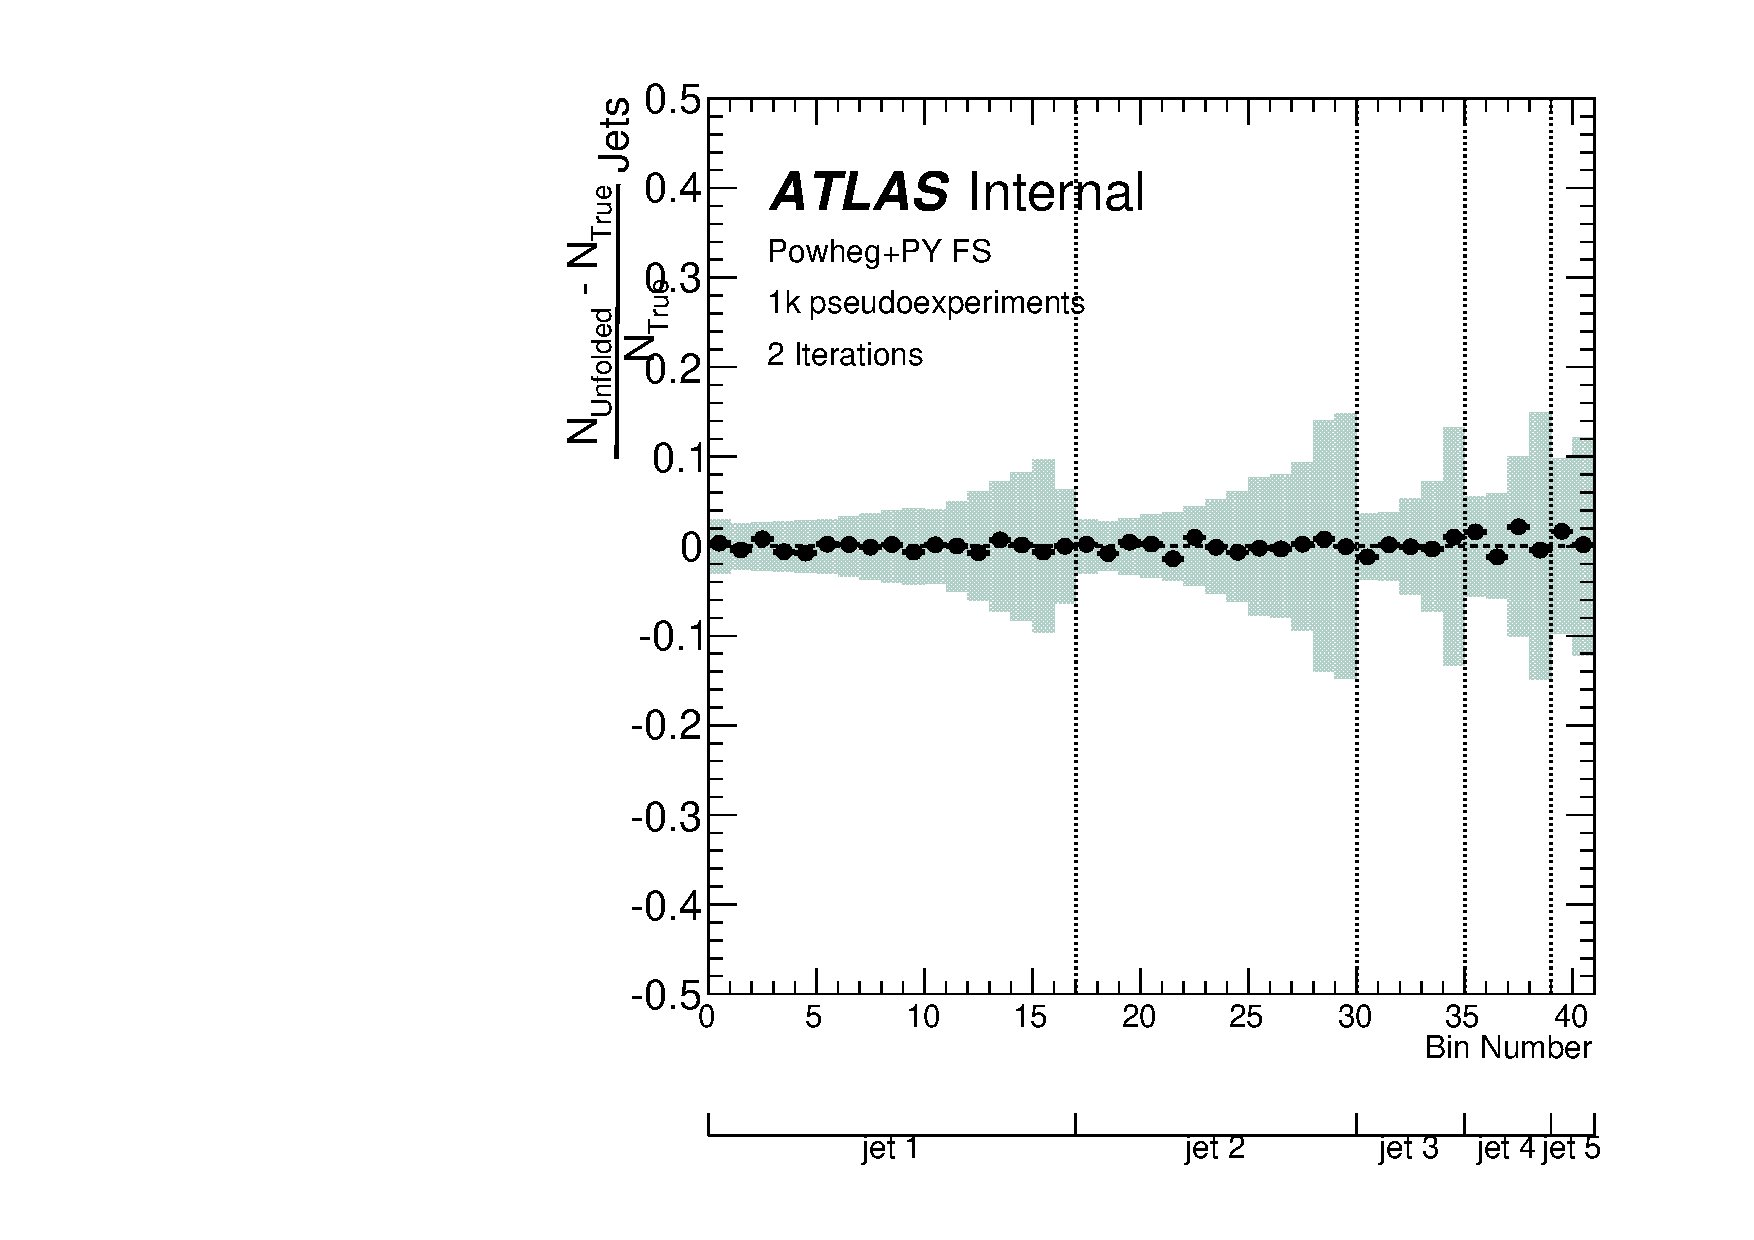
\includegraphics[width=\textwidth]{fig/Stress/117050fullsim/FracBias2Iterations.pdf}
\end{subfigure}
\\
\begin{subfigure}[]{0.5\textwidth}
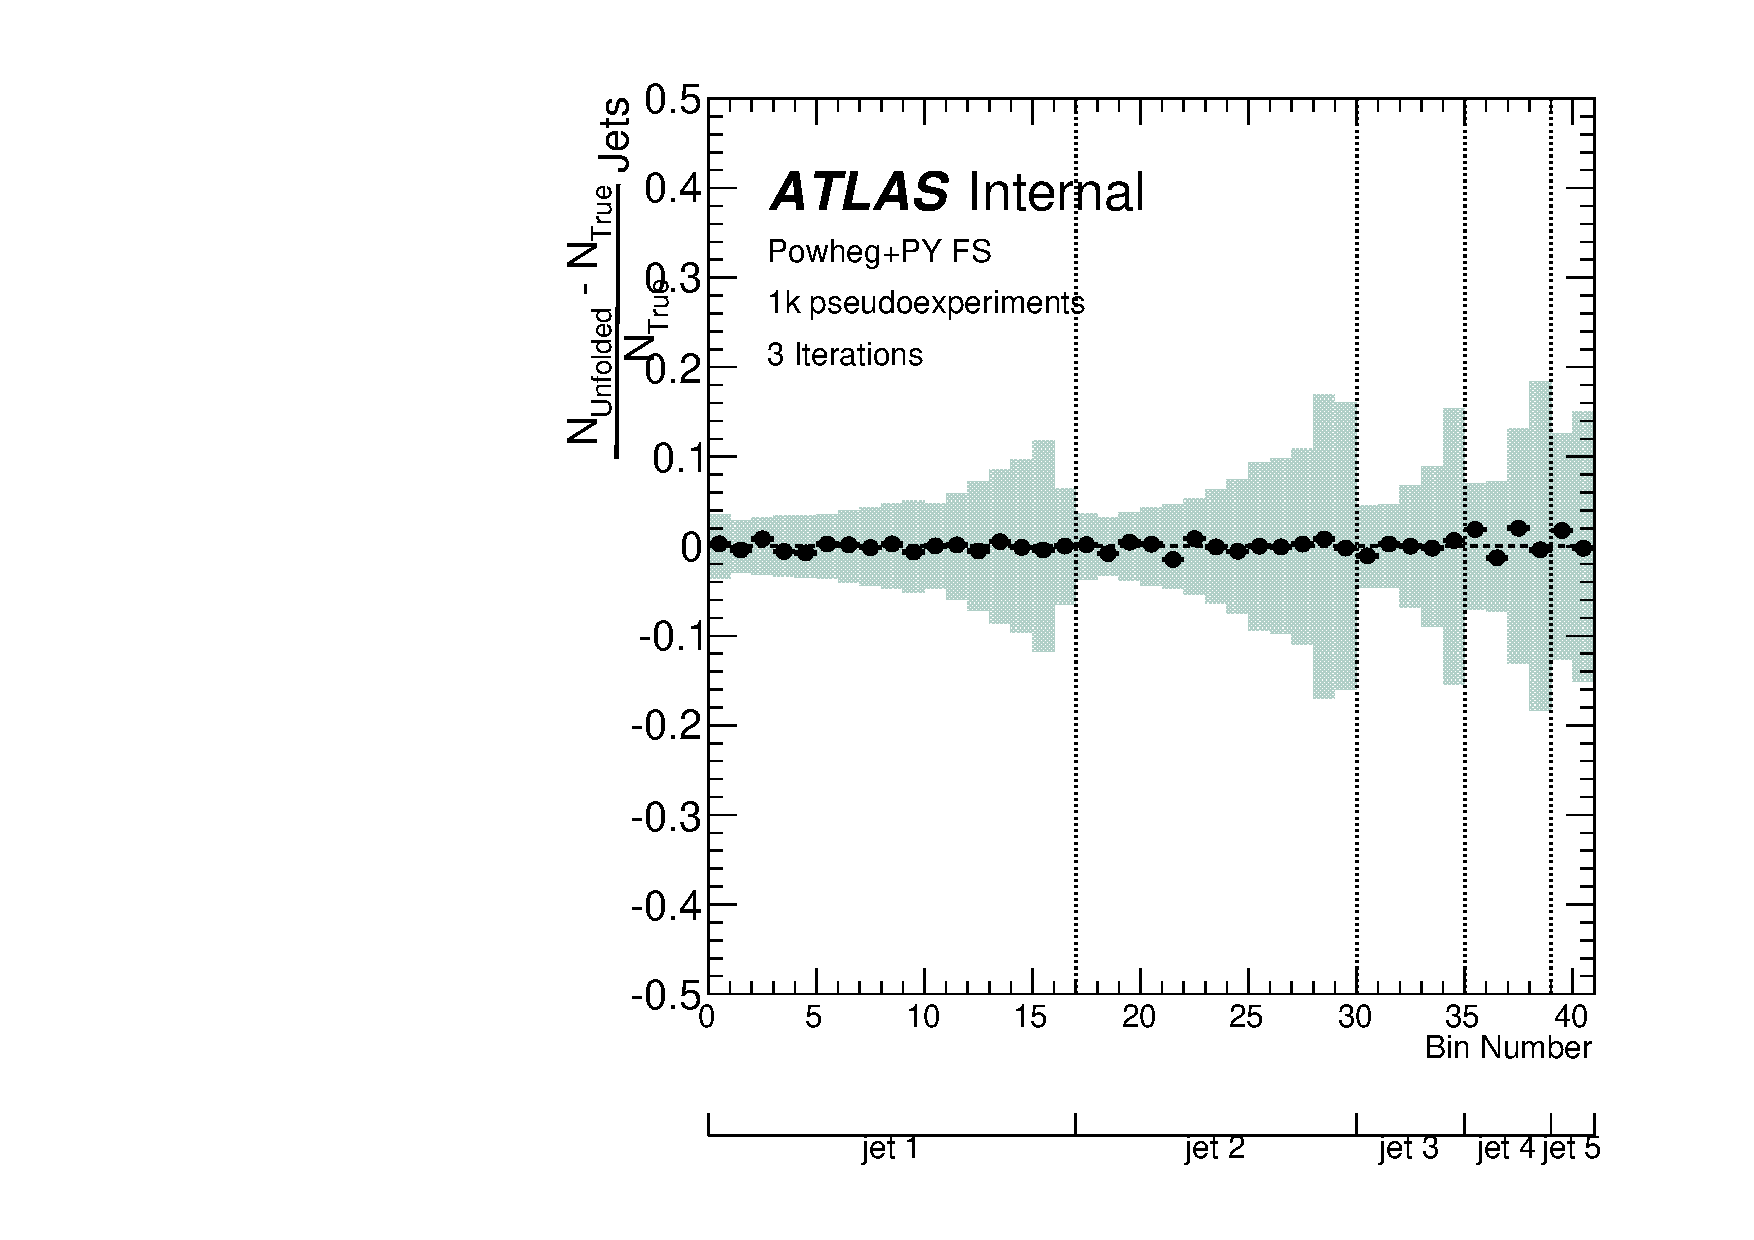
\includegraphics[width=\textwidth]{fig/Stress/117050fullsim/FracBias3Iterations.pdf}
\end{subfigure}
~
\begin{subfigure}[]{0.5\textwidth}
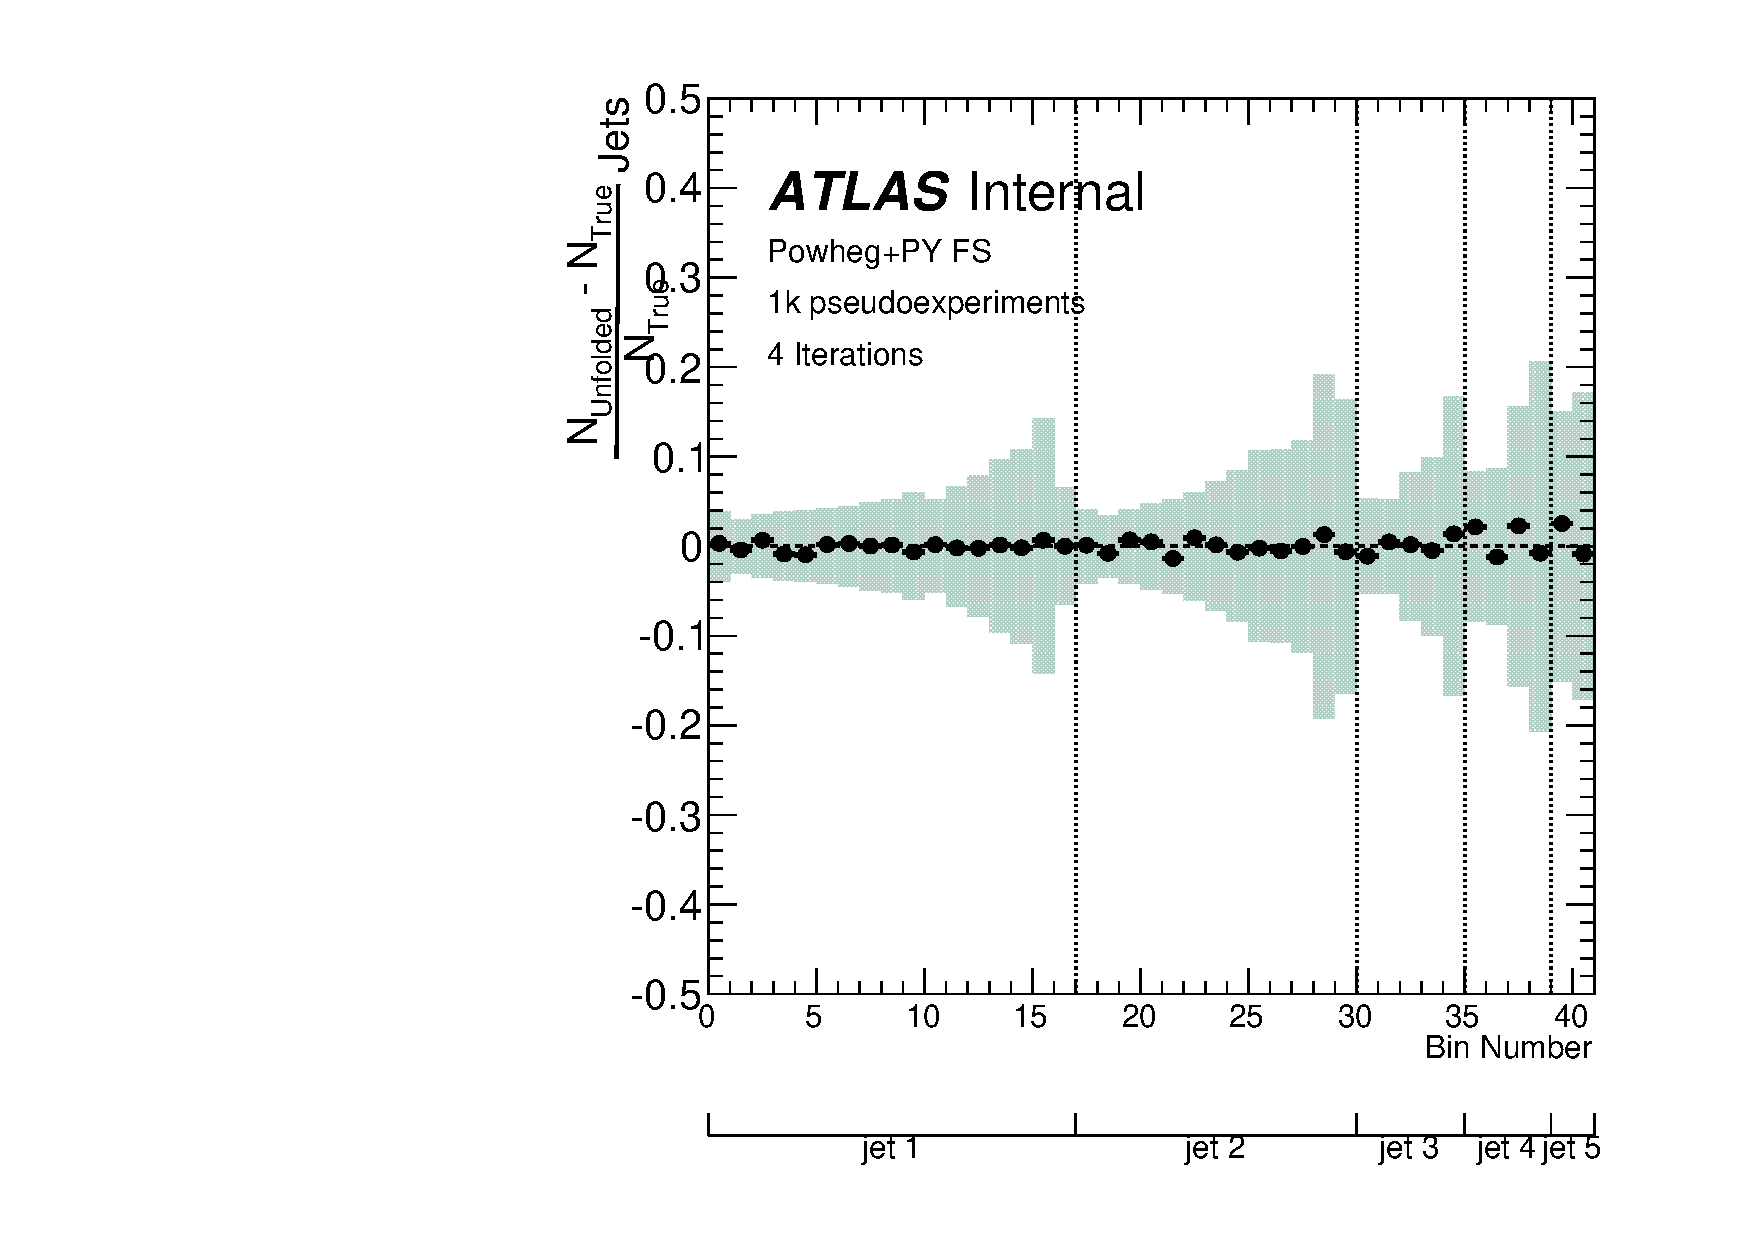
\includegraphics[width=\textwidth]{fig/Stress/117050fullsim/FracBias4Iterations.pdf}
\end{subfigure}
\caption{Fractional bias distribution for pseudoexperiments constructed from \newline \powpy\ fullsim simulation unfolded against a matrix filled with the baseline simulation. One thousand pseudoexperiments, each the size of the events in data, are selected from the sample and unfolded. The Bayesian unfolding method with various numbers of iterations is used. Each bin of the distribution over the pseudoexperiments is fit with a gaussian. The black points show the fitted mean of each bin and the blue band shows the fitted sigma.}
\label{fig:fsfrbias}
\end{figure}
\clearpage
\begin{figure}
\begin{subfigure}[]{0.5\textwidth}
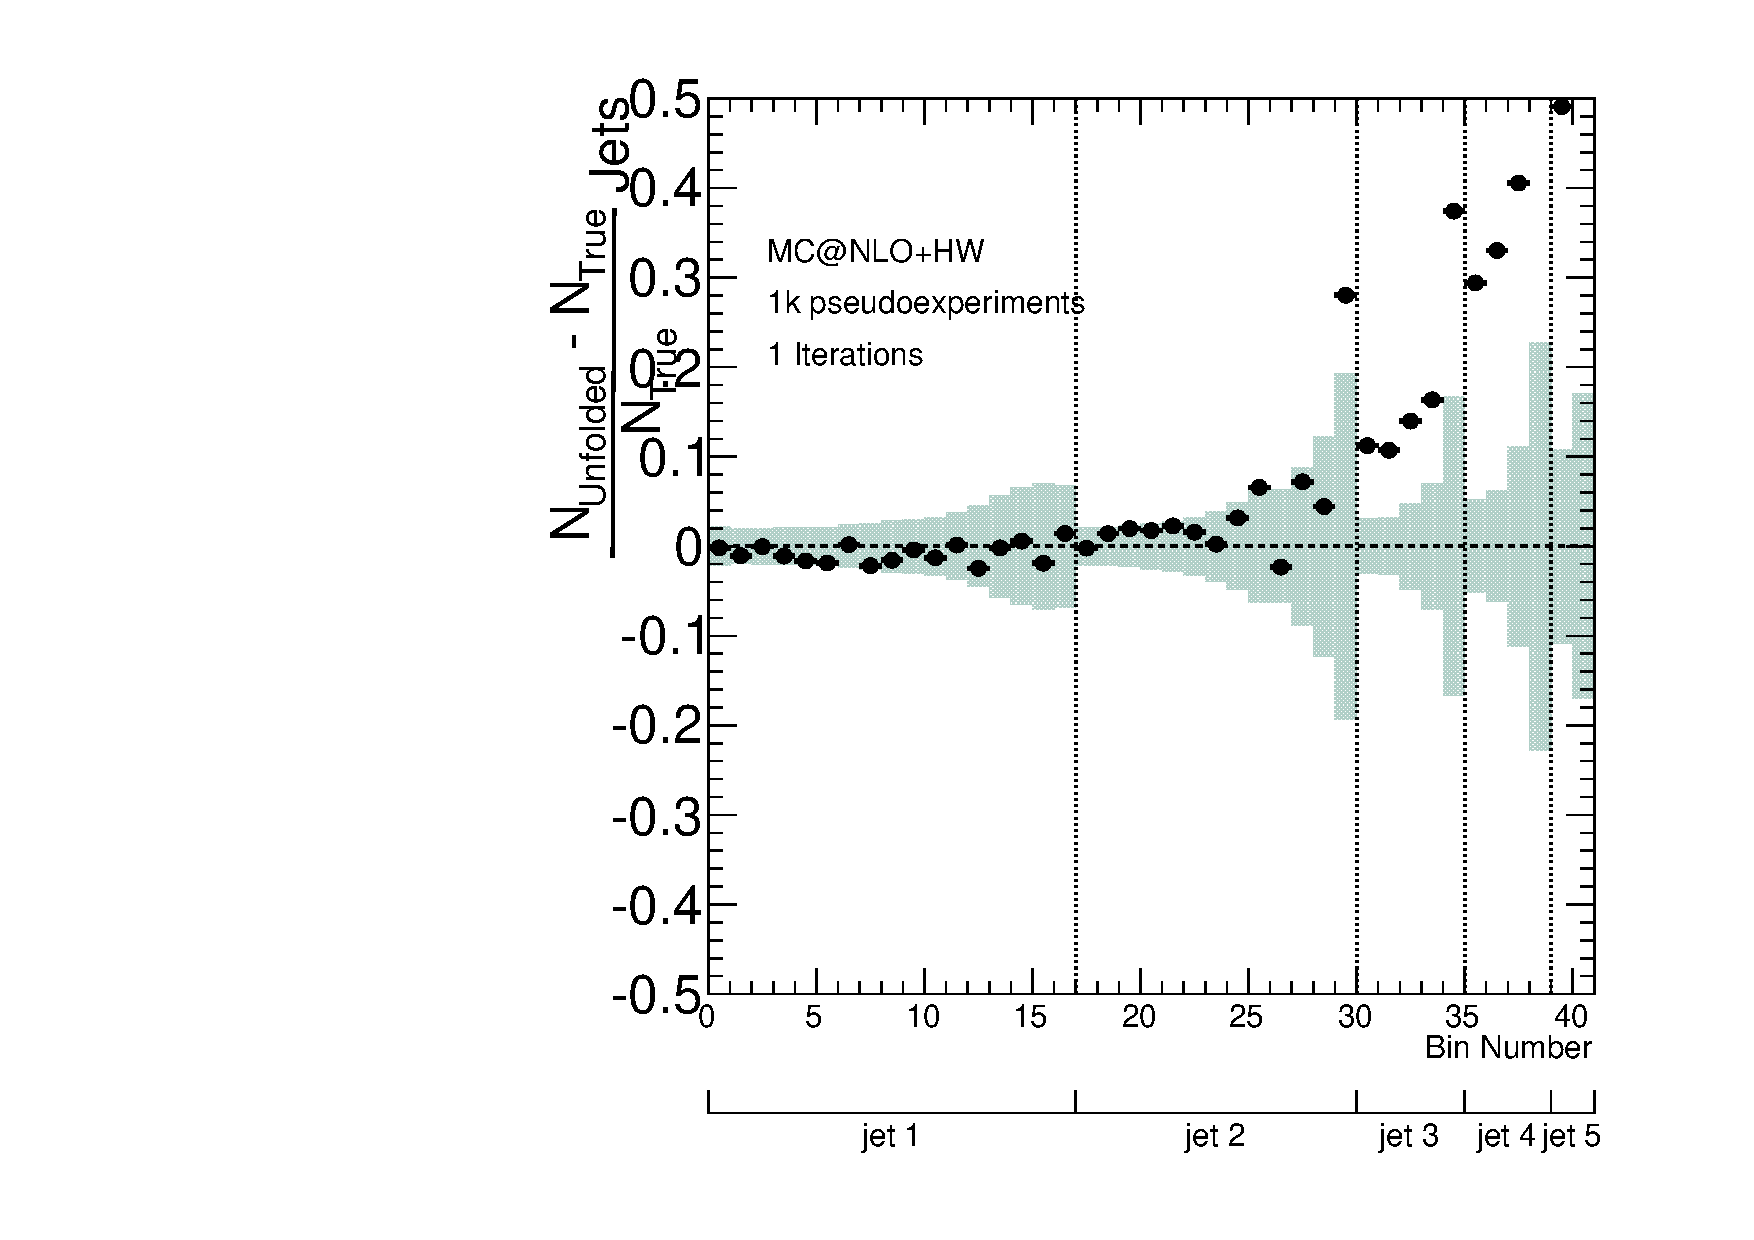
\includegraphics[width=\textwidth]{fig/Stress/105200atlfast/FracBias1Iterations.pdf}
\end{subfigure}
\begin{subfigure}[]{0.5\textwidth}
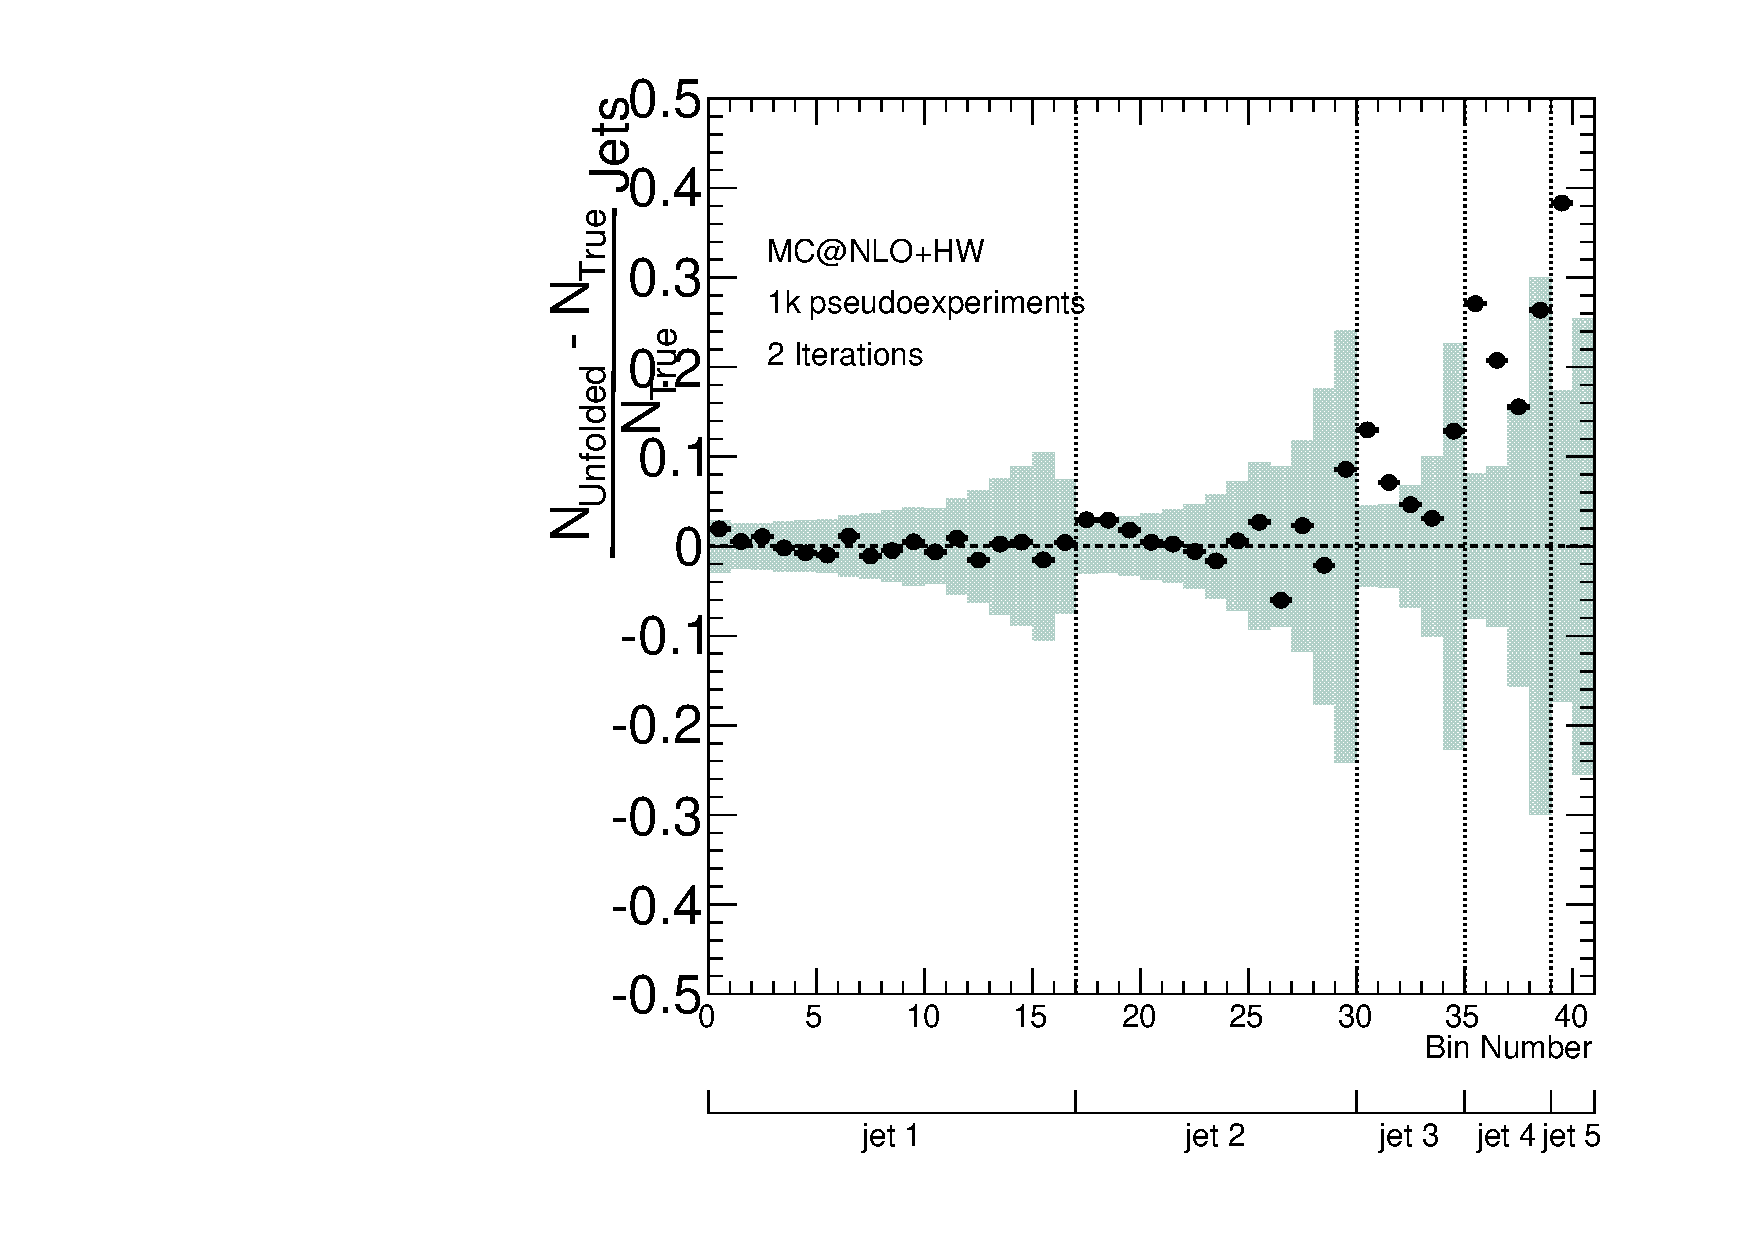
\includegraphics[width=\textwidth]{fig/Stress/105200atlfast/FracBias2Iterations.pdf}
\end{subfigure}
\\
\begin{subfigure}[]{0.5\textwidth}
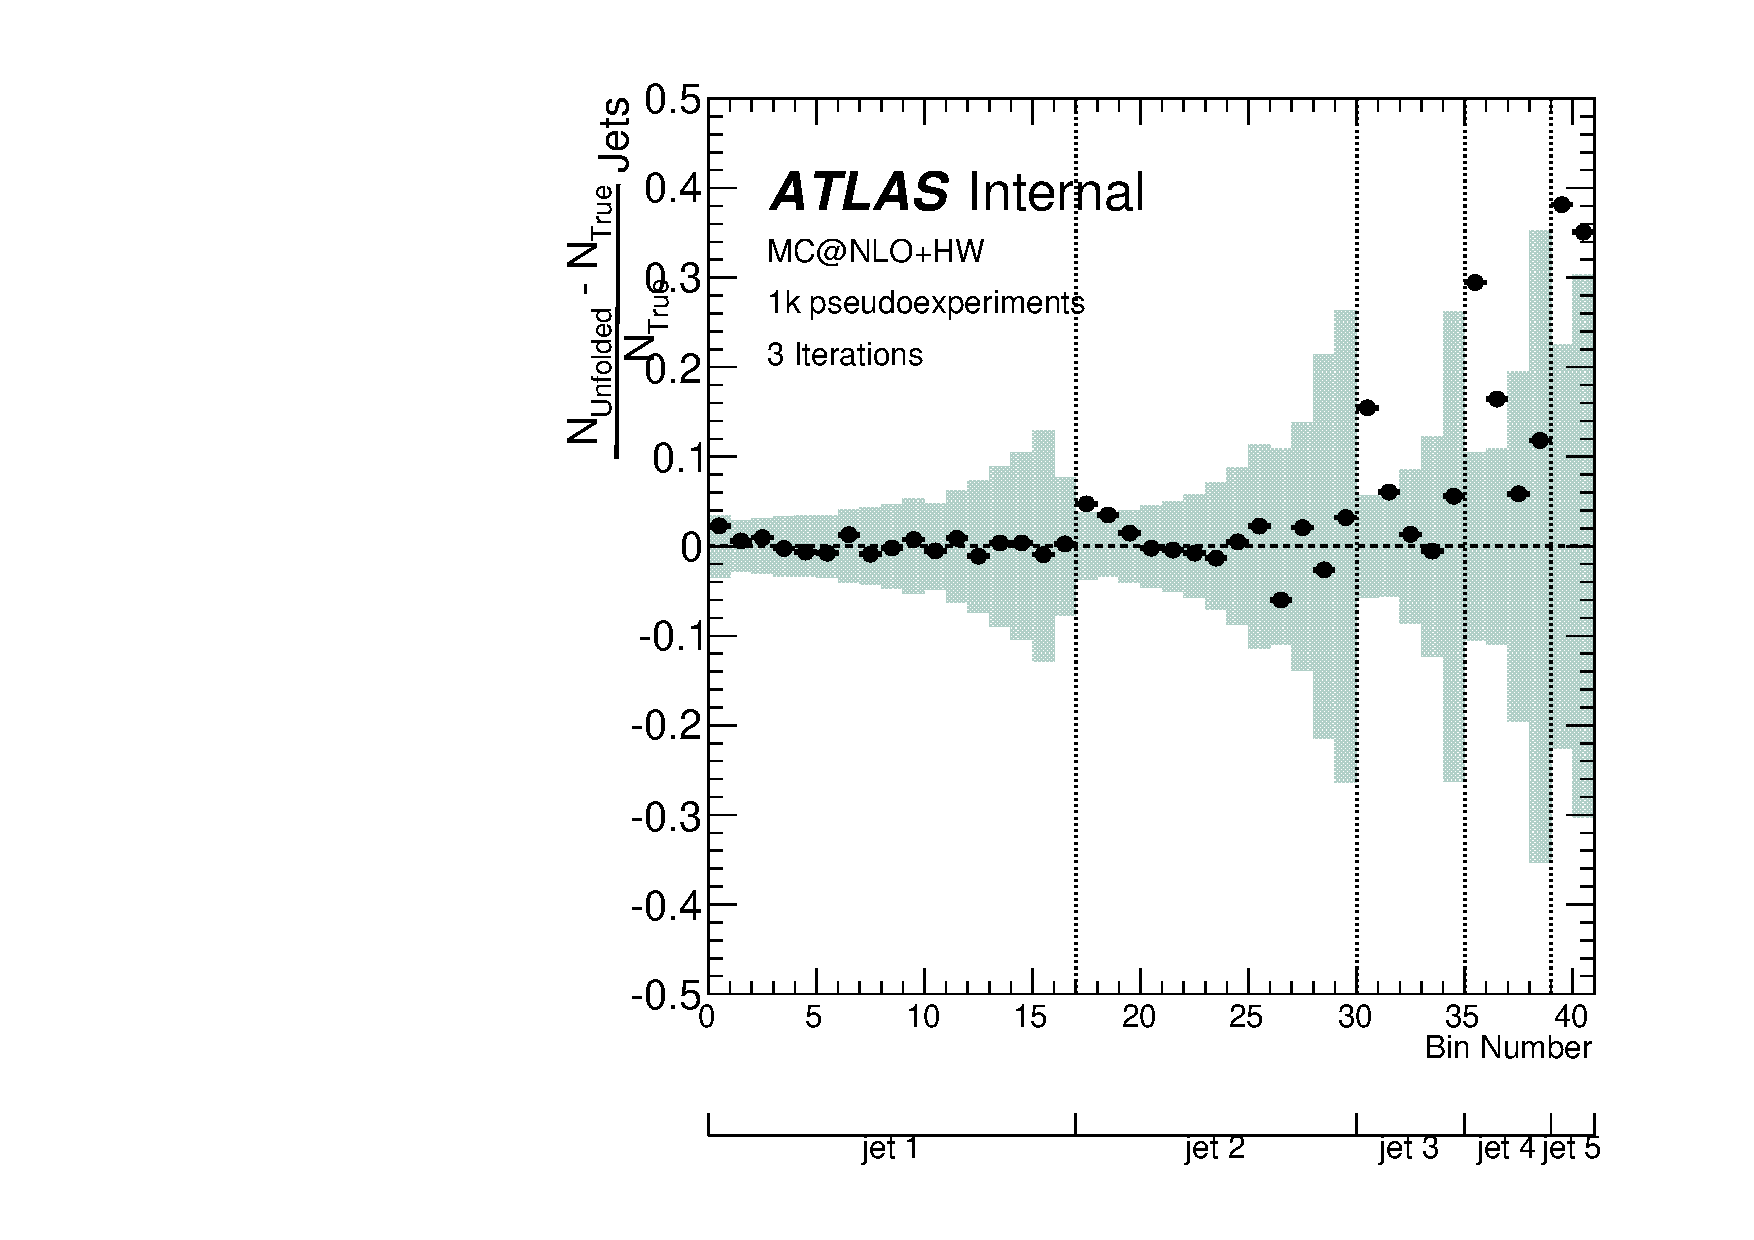
\includegraphics[width=\textwidth]{fig/Stress/105200atlfast/FracBias3Iterations.pdf}
\end{subfigure}
\begin{subfigure}[]{0.5\textwidth}
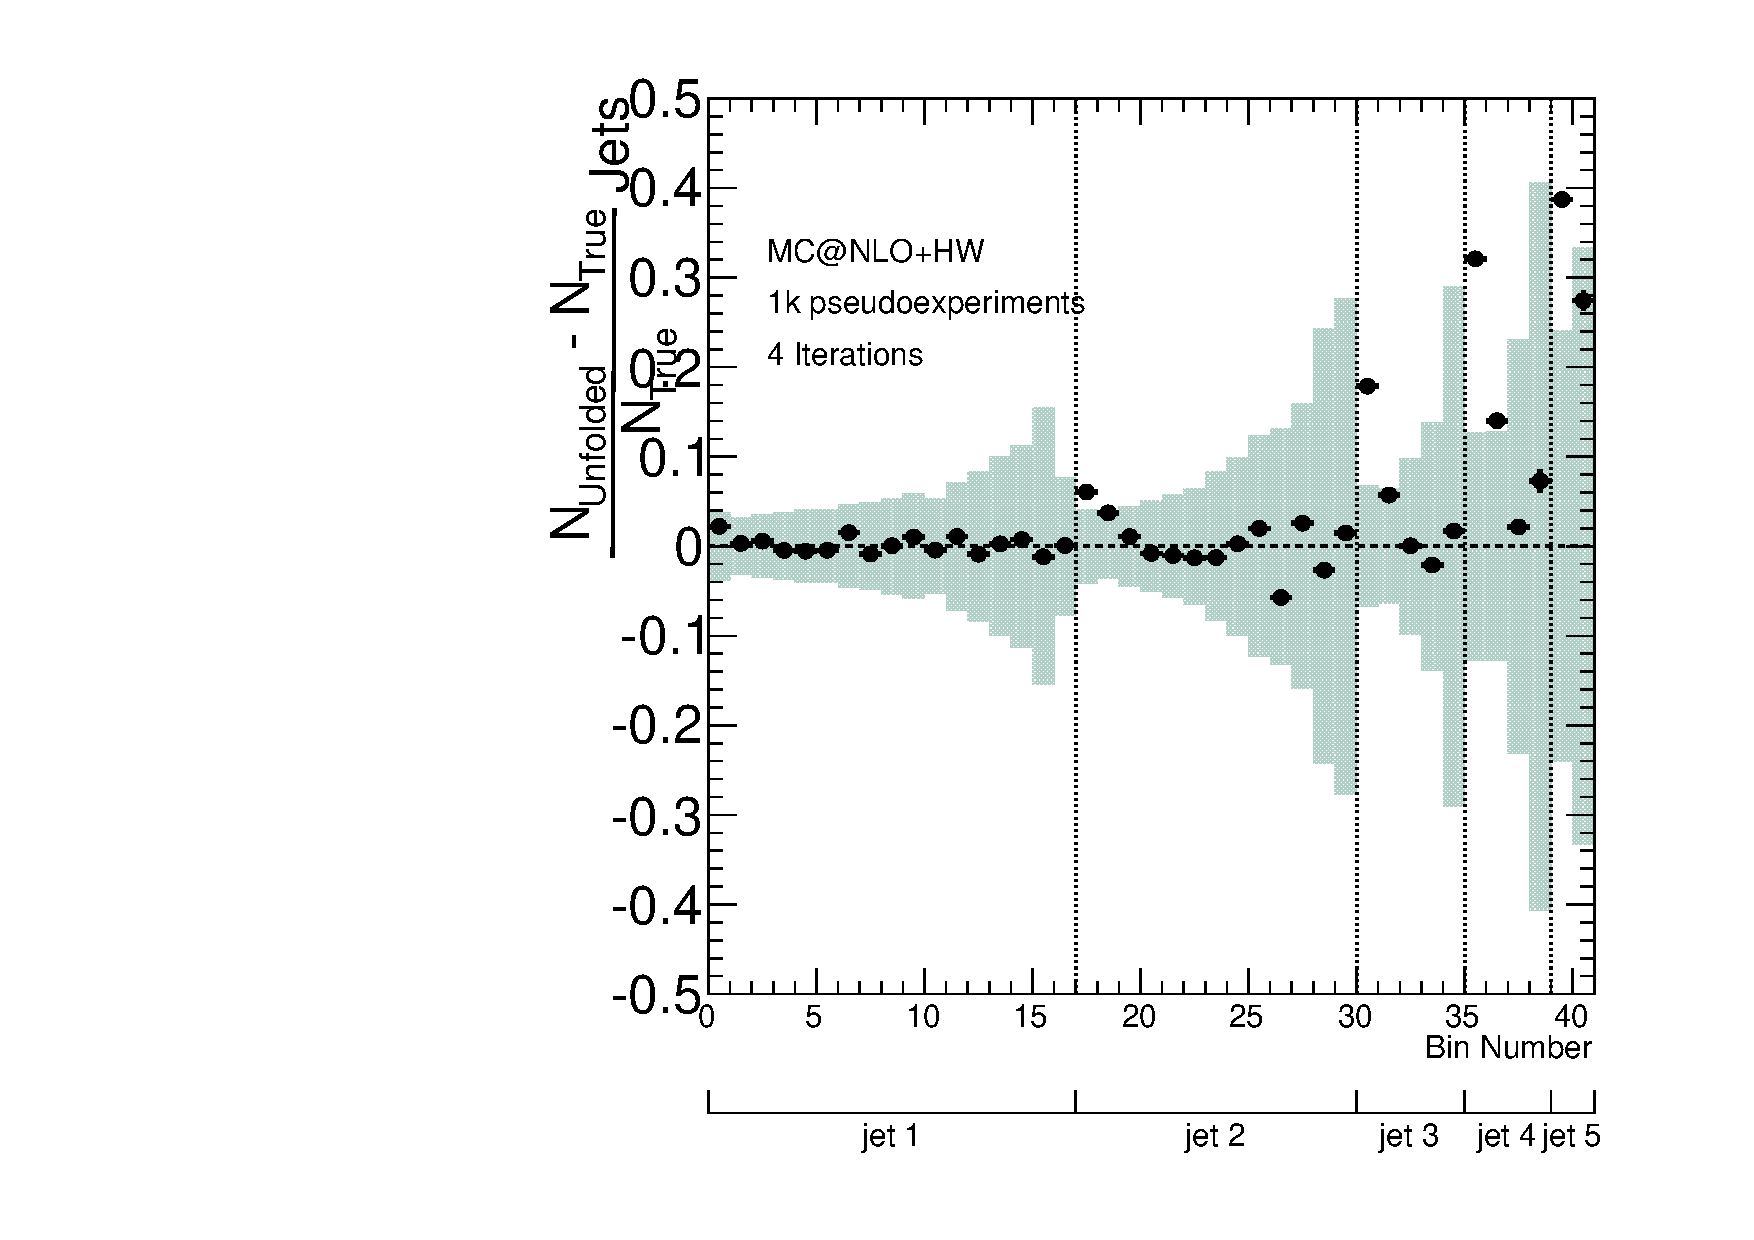
\includegraphics[width=\textwidth]{fig/Stress/105200atlfast/FracBias4Iterations.pdf}
\end{subfigure}
\caption{Fractional bias distribution for pseudoexperiments constructed from \newline \mcnlohw\ simulation unfolded against a matrix filled with the baseline simulation. One thousand pseudoexperiments, each the size of the events in data, are selected from the sample and unfolded. The Bayesian unfolding method with various numbers of iterations is used. Each bin of the distribution over the pseudoexperiments is fit with a gaussian. The black points show the fitted mean of each bin and the blue band shows the fitted sigma. }
\label{fig:mcnlohwfrbias}
\end{figure}
\clearpage
%\section{Pull \pow+\hw}
\begin{figure}
\begin{subfigure}[]{0.5\textwidth}
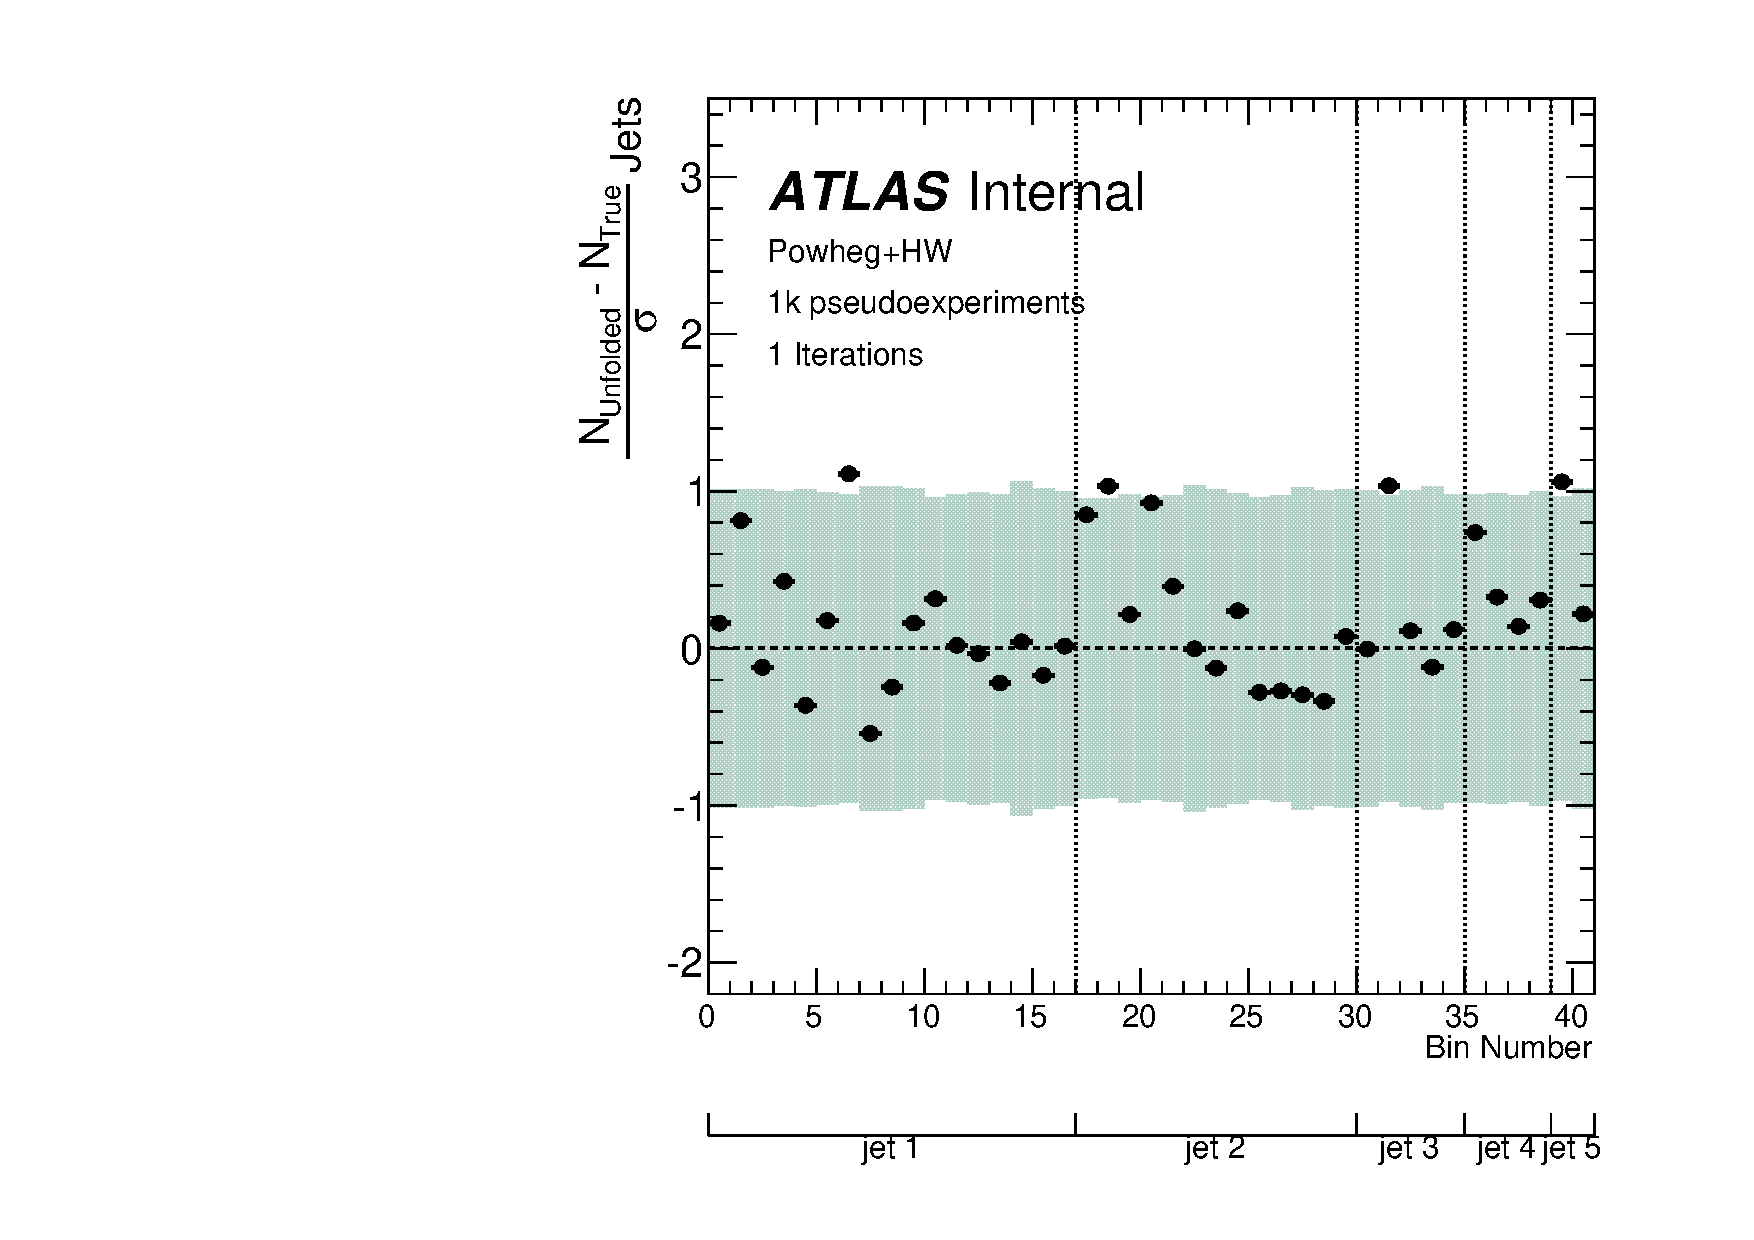
\includegraphics[width=\textwidth]{fig/Stress/105860atlfast/Pull1Iterations.pdf}
\end{subfigure}
~
\begin{subfigure}[]{0.5\textwidth}
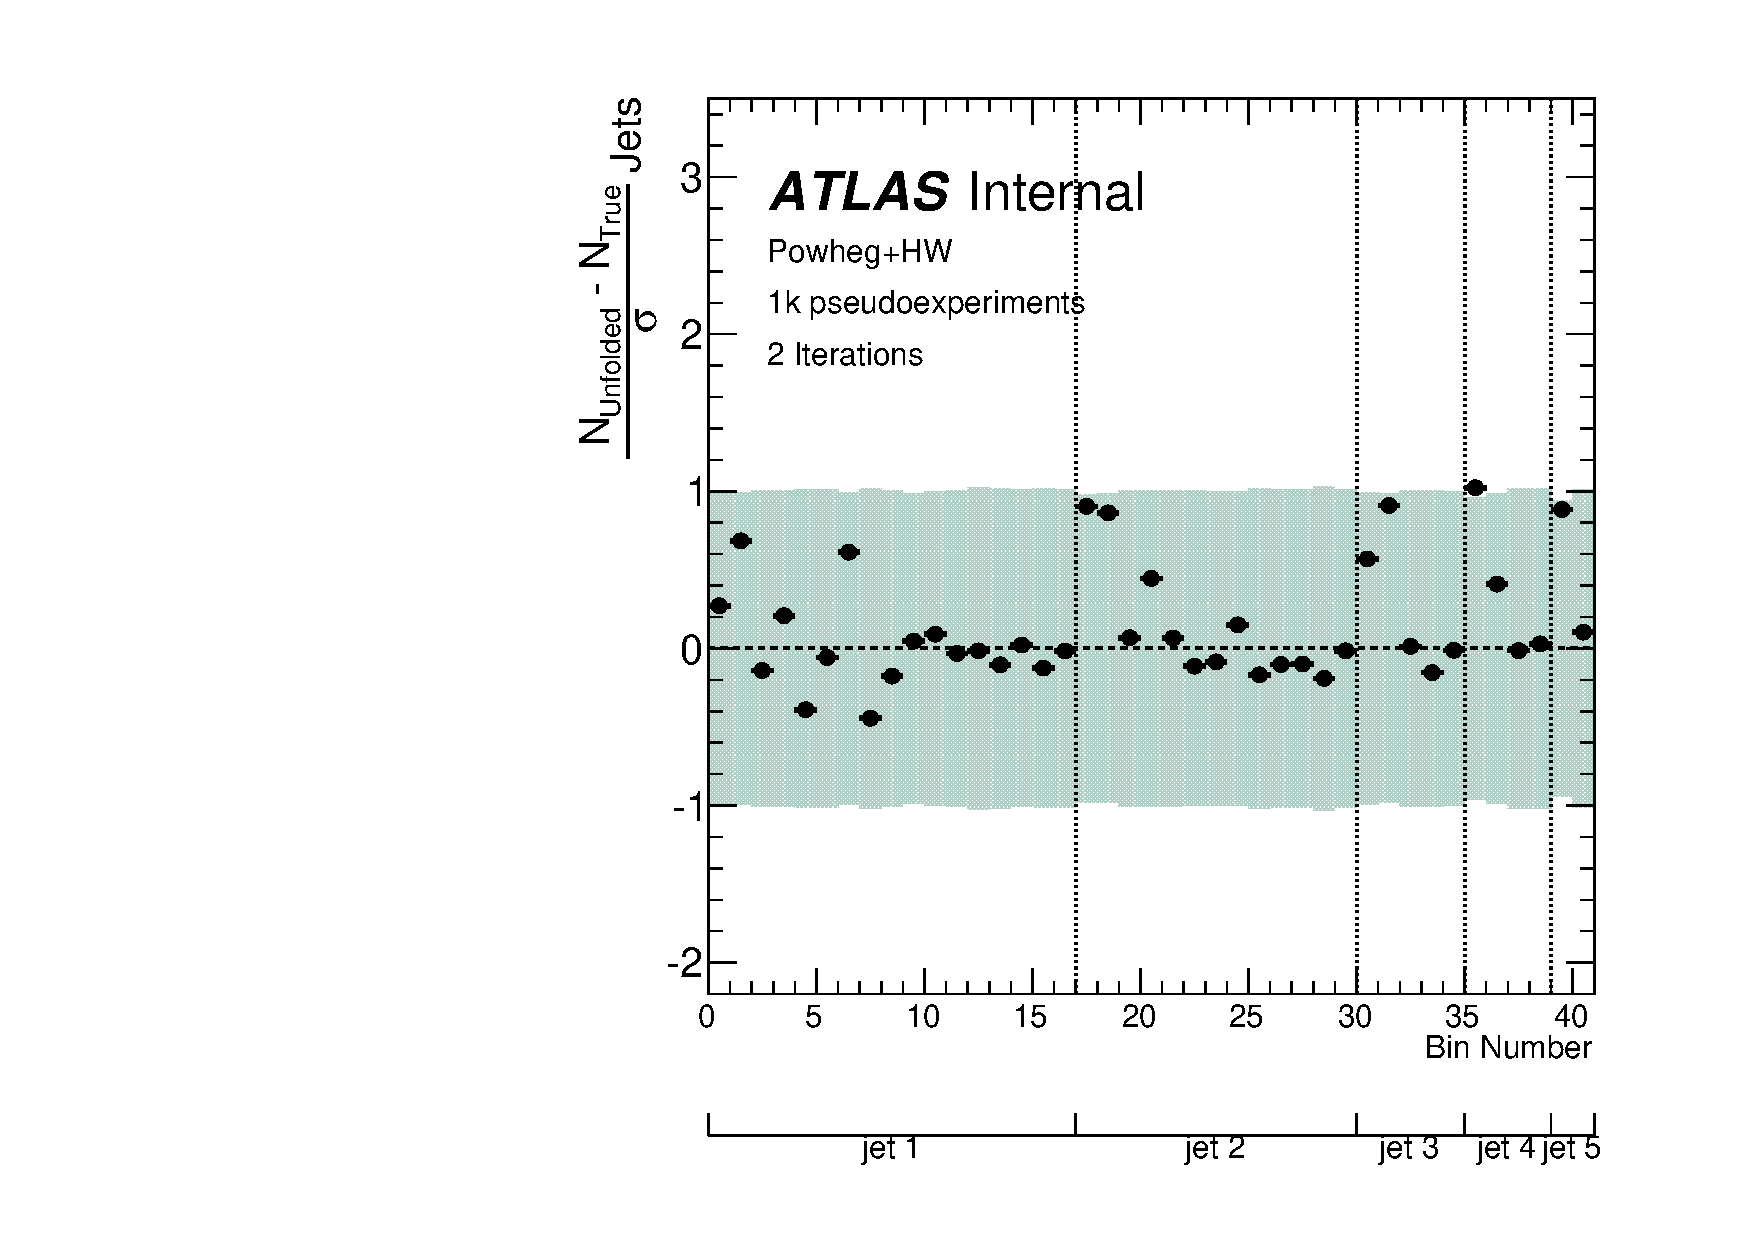
\includegraphics[width=\textwidth]{fig/Stress/105860atlfast/Pull2Iterations.pdf}
\end{subfigure}
\\
\begin{subfigure}[]{0.5\textwidth}
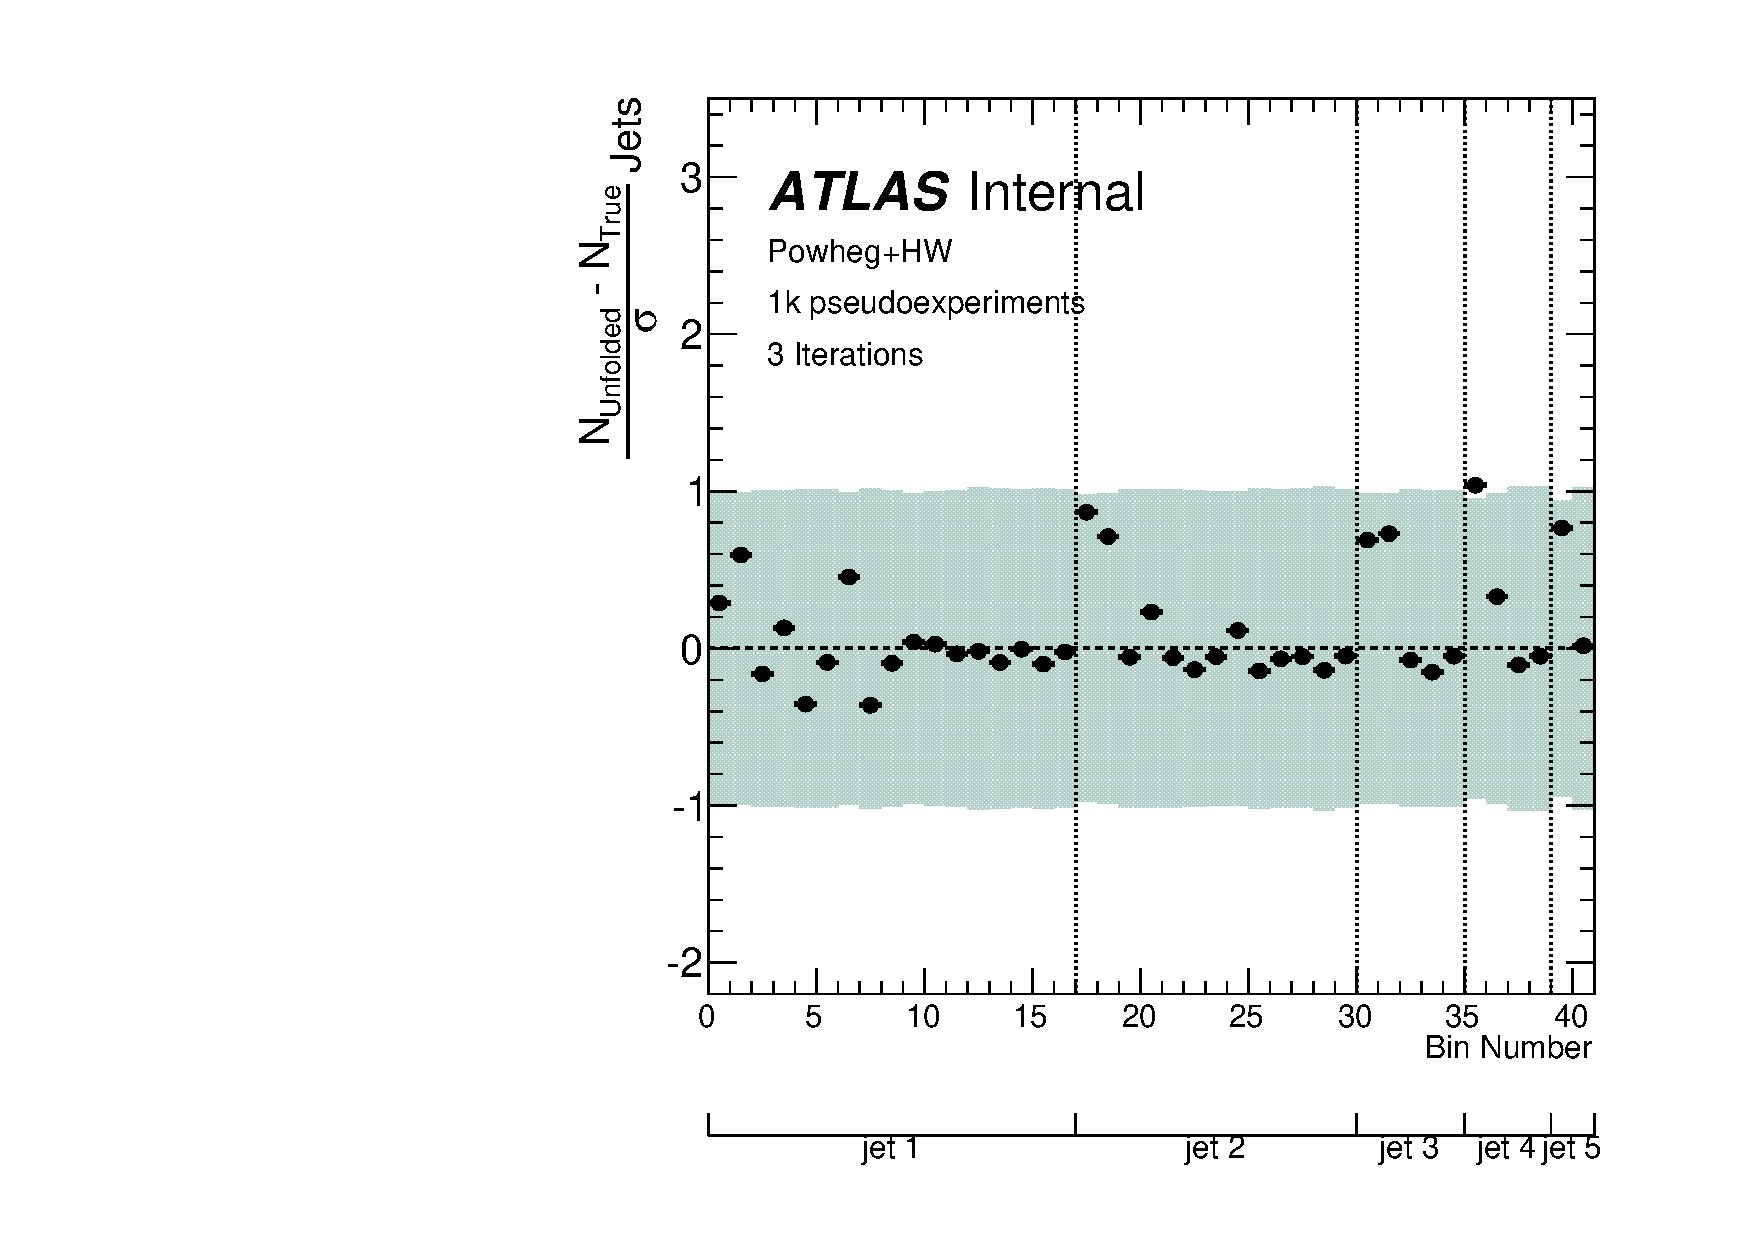
\includegraphics[width=\textwidth]{fig/Stress/105860atlfast/Pull3Iterations.pdf}
\end{subfigure}
~
\begin{subfigure}[]{0.5\textwidth}
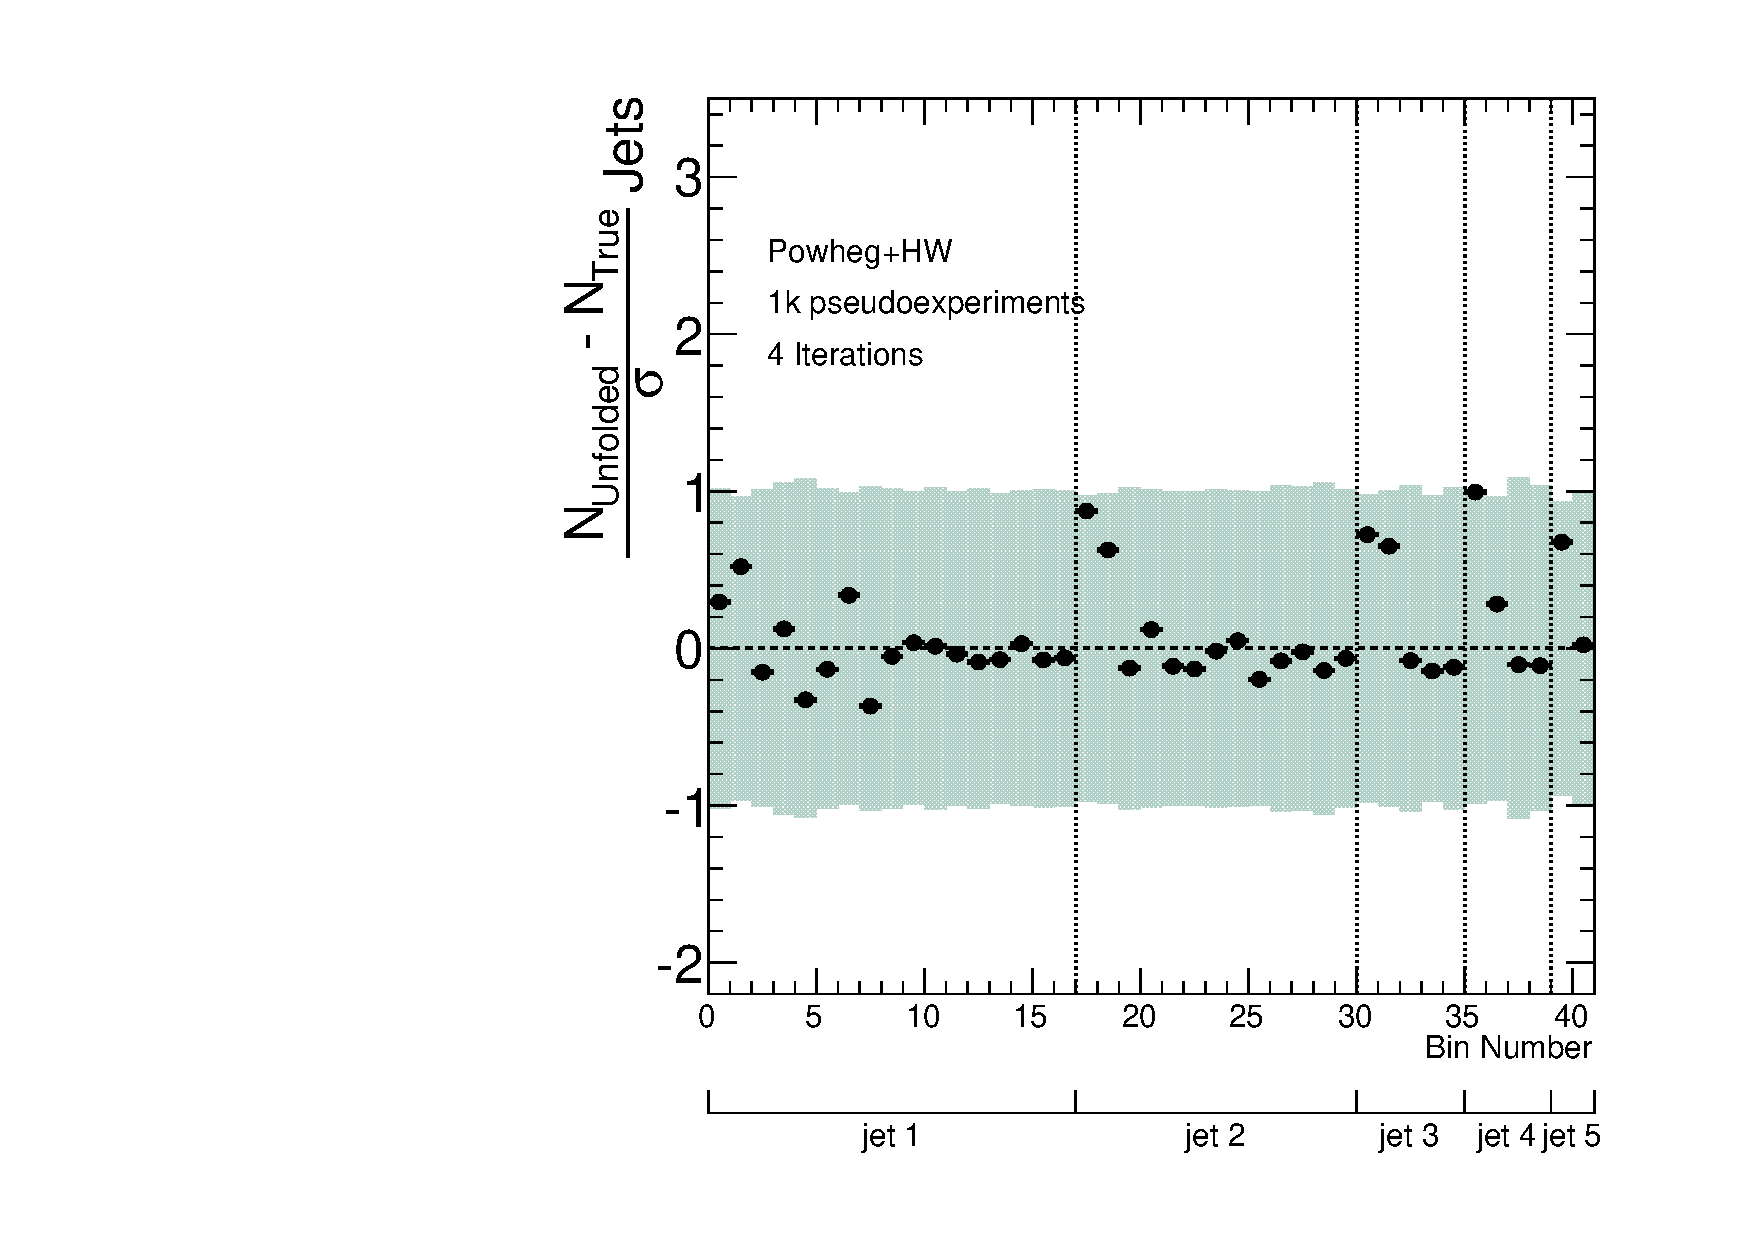
\includegraphics[width=\textwidth]{fig/Stress/105860atlfast/Pull4Iterations.pdf}
\end{subfigure}
\caption{Pull distribution for pseudoexperiments constructed from \newline \pow+\hw~ simulation unfolded against a matrix filled with the baseline simulation. One thousand pseudoexperiments, each the size of the events in data, are selected from the sample and unfolded. The Bayesian unfolding method with various numbers of iterations is used. Each bin of the distribution over the pseudoexperiments is fit with a gaussian. The black points show the fitted mean of each bin and the blue band shows the fitted sigma.}
\label{fig:powhwpull}
\end{figure}
\clearpage
%\section{Pull \hdamp}
\begin{figure}
\begin{subfigure}[]{0.5\textwidth}
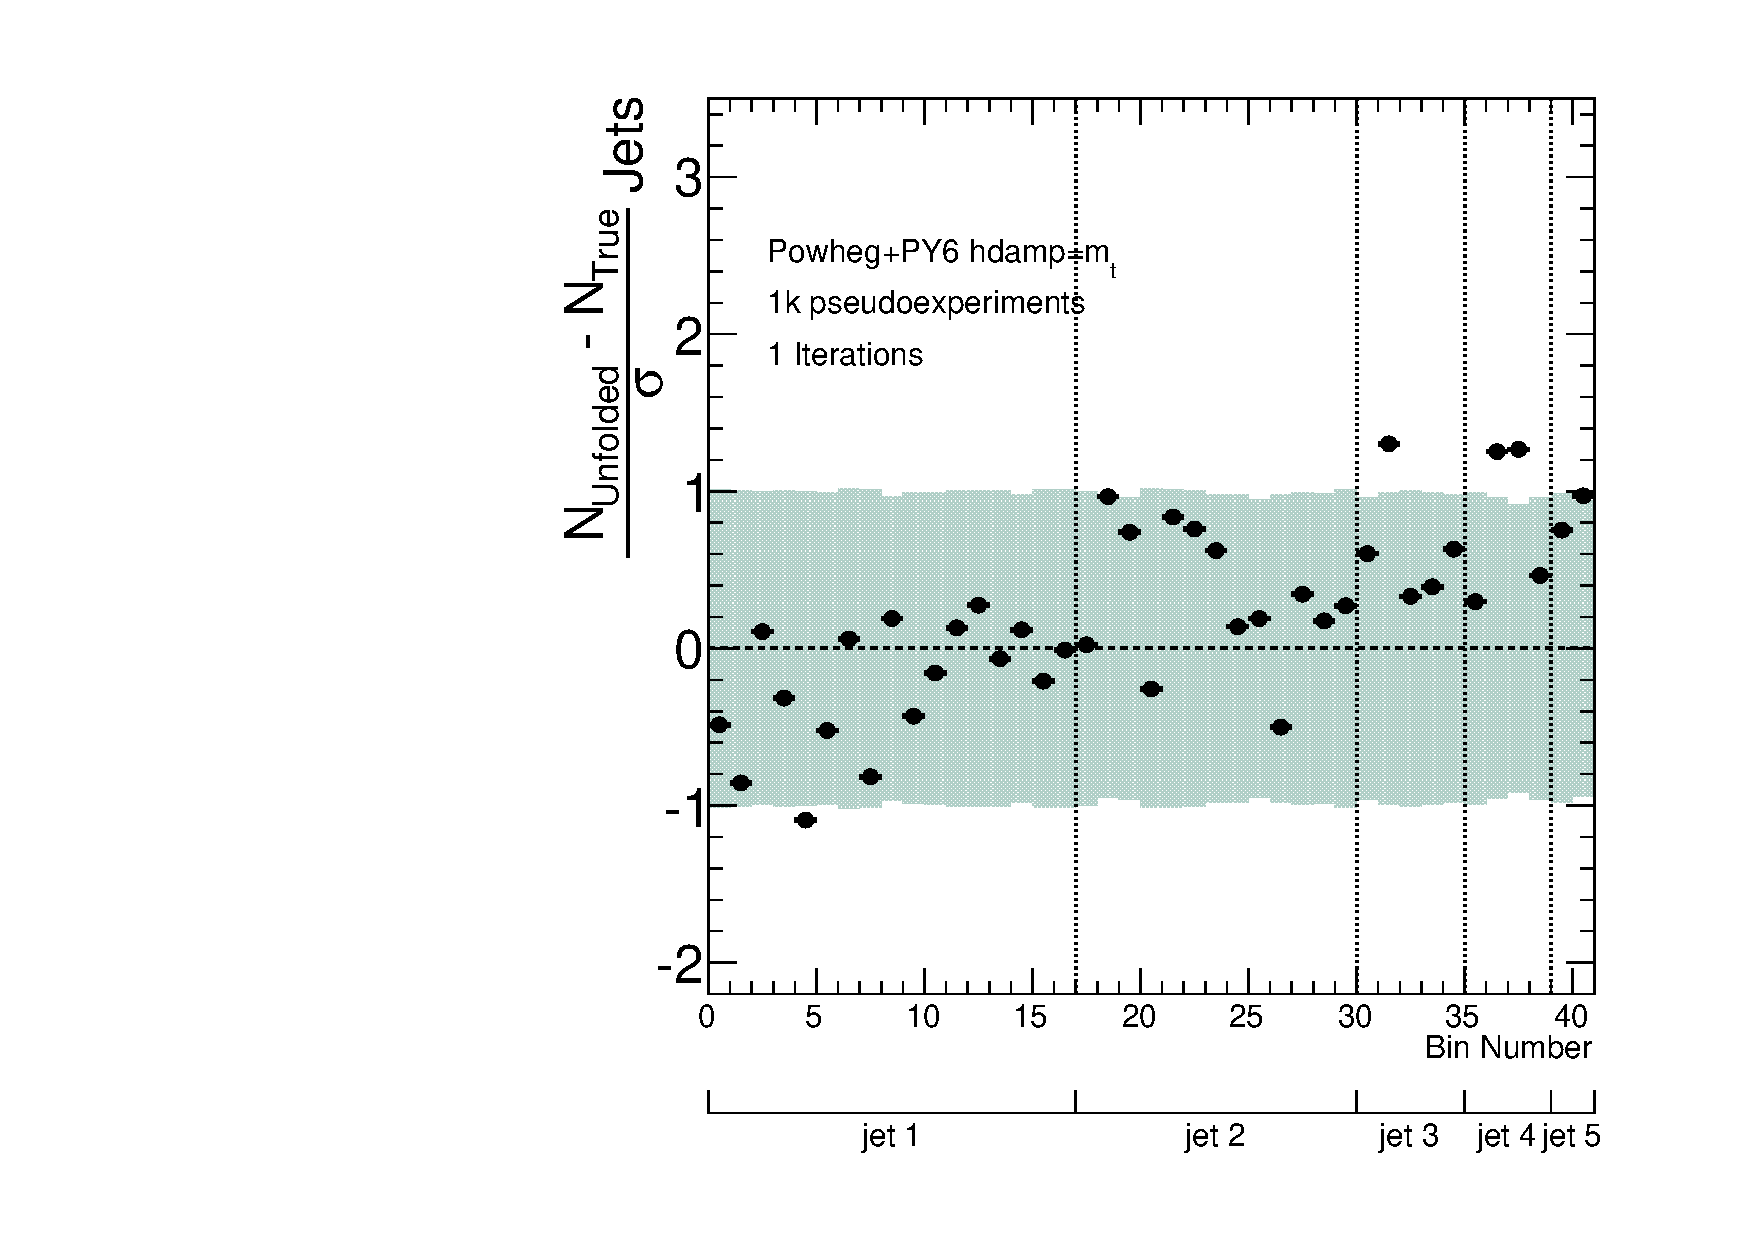
\includegraphics[width=\textwidth]{fig/Stress/110404atlfast/Pull1Iterations.pdf}
\end{subfigure}
~
\begin{subfigure}[]{0.5\textwidth}
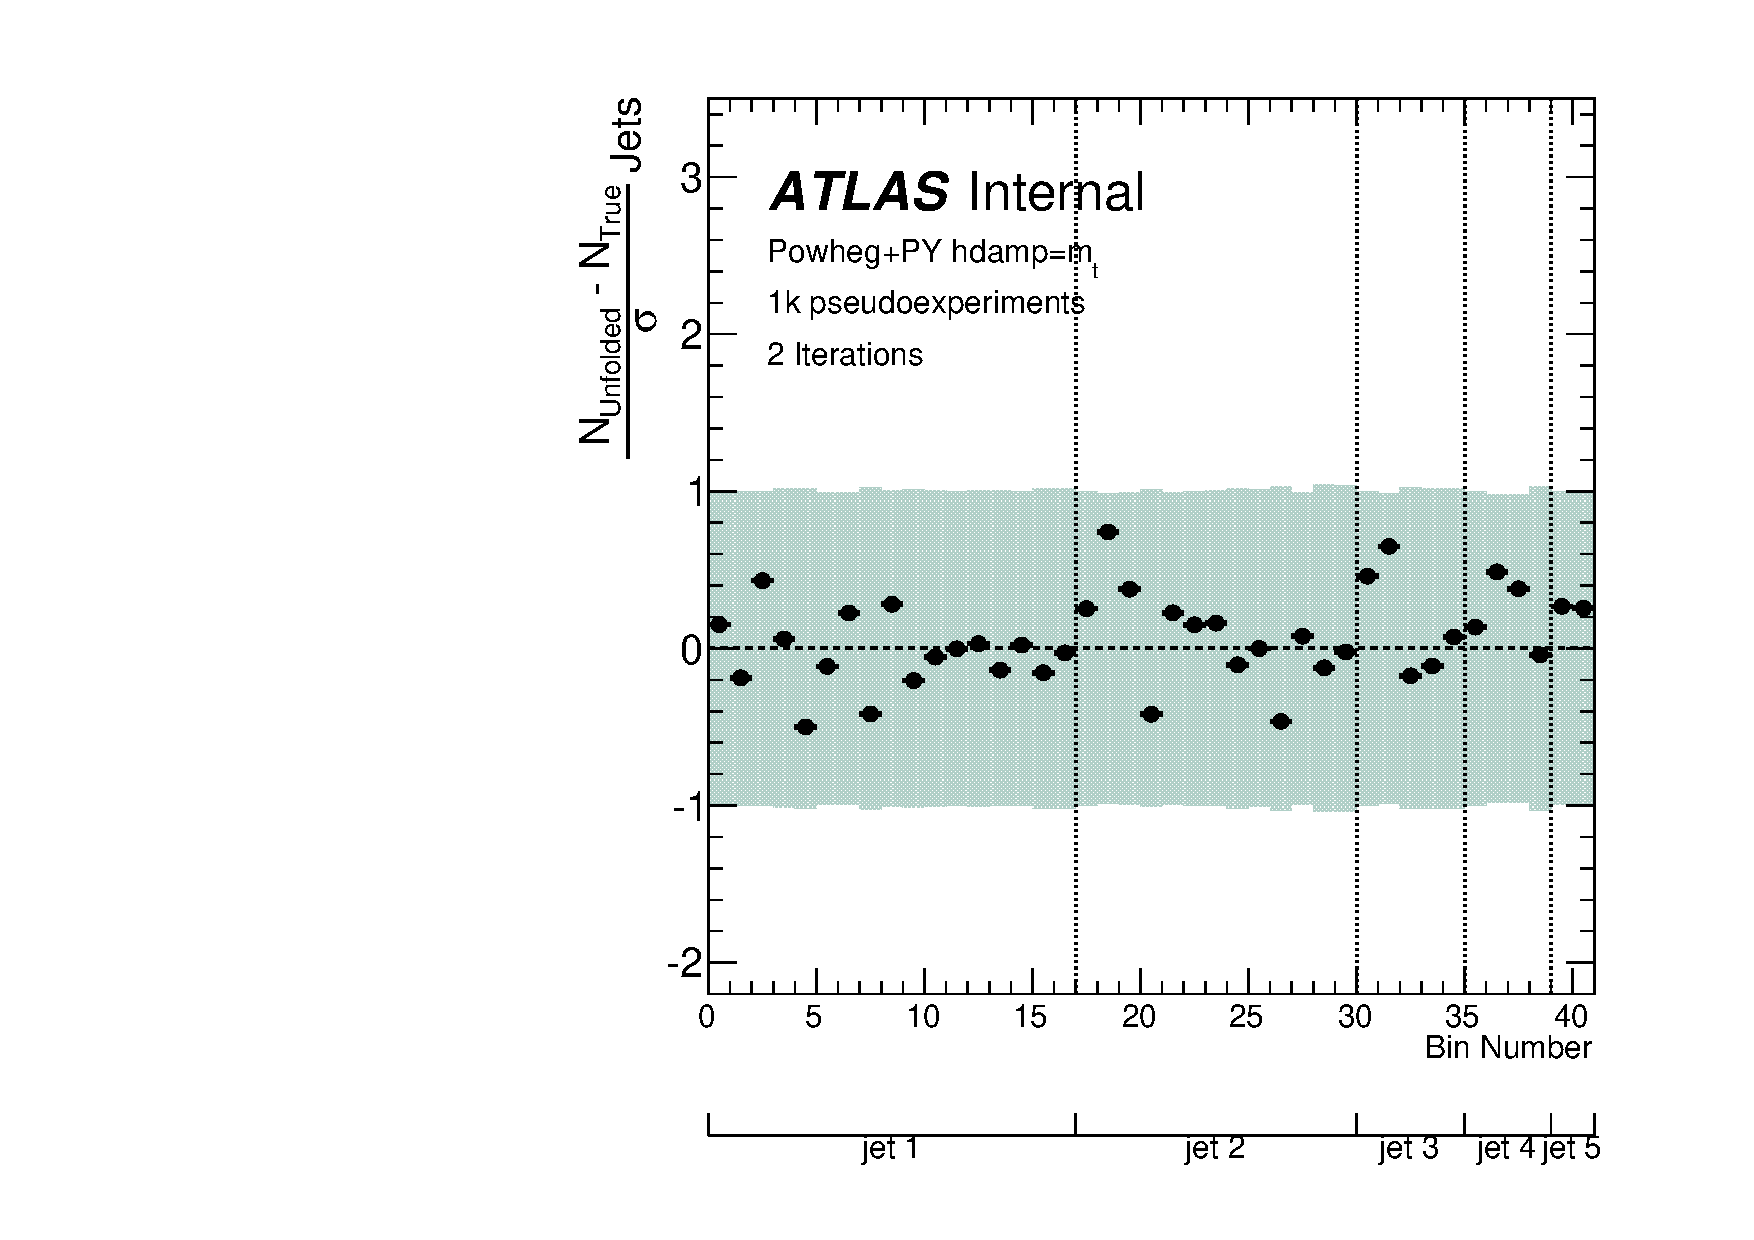
\includegraphics[width=\textwidth]{fig/Stress/110404atlfast/Pull2Iterations.pdf}
\end{subfigure}
\\
\begin{subfigure}[]{0.5\textwidth}
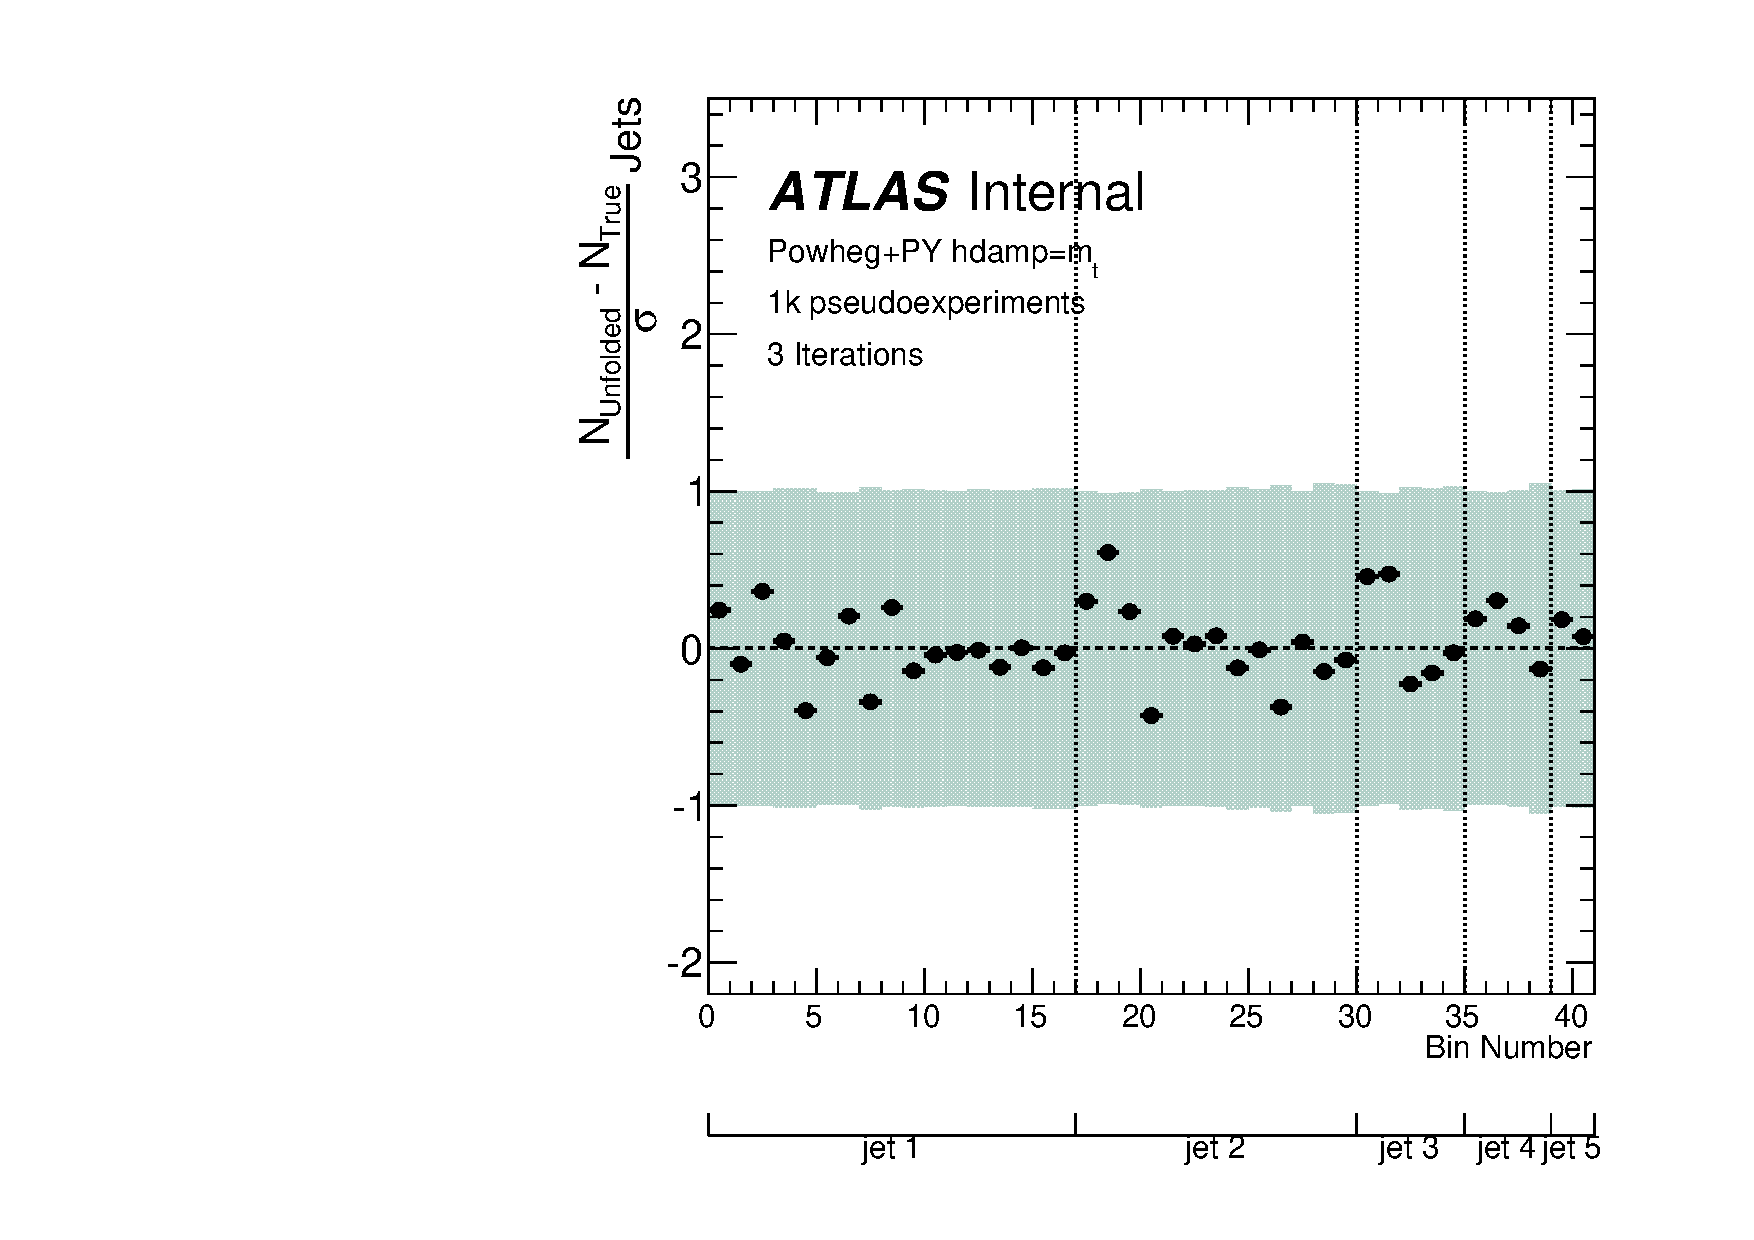
\includegraphics[width=\textwidth]{fig/Stress/110404atlfast/Pull3Iterations.pdf}
\end{subfigure}
~
\begin{subfigure}[]{0.5\textwidth}
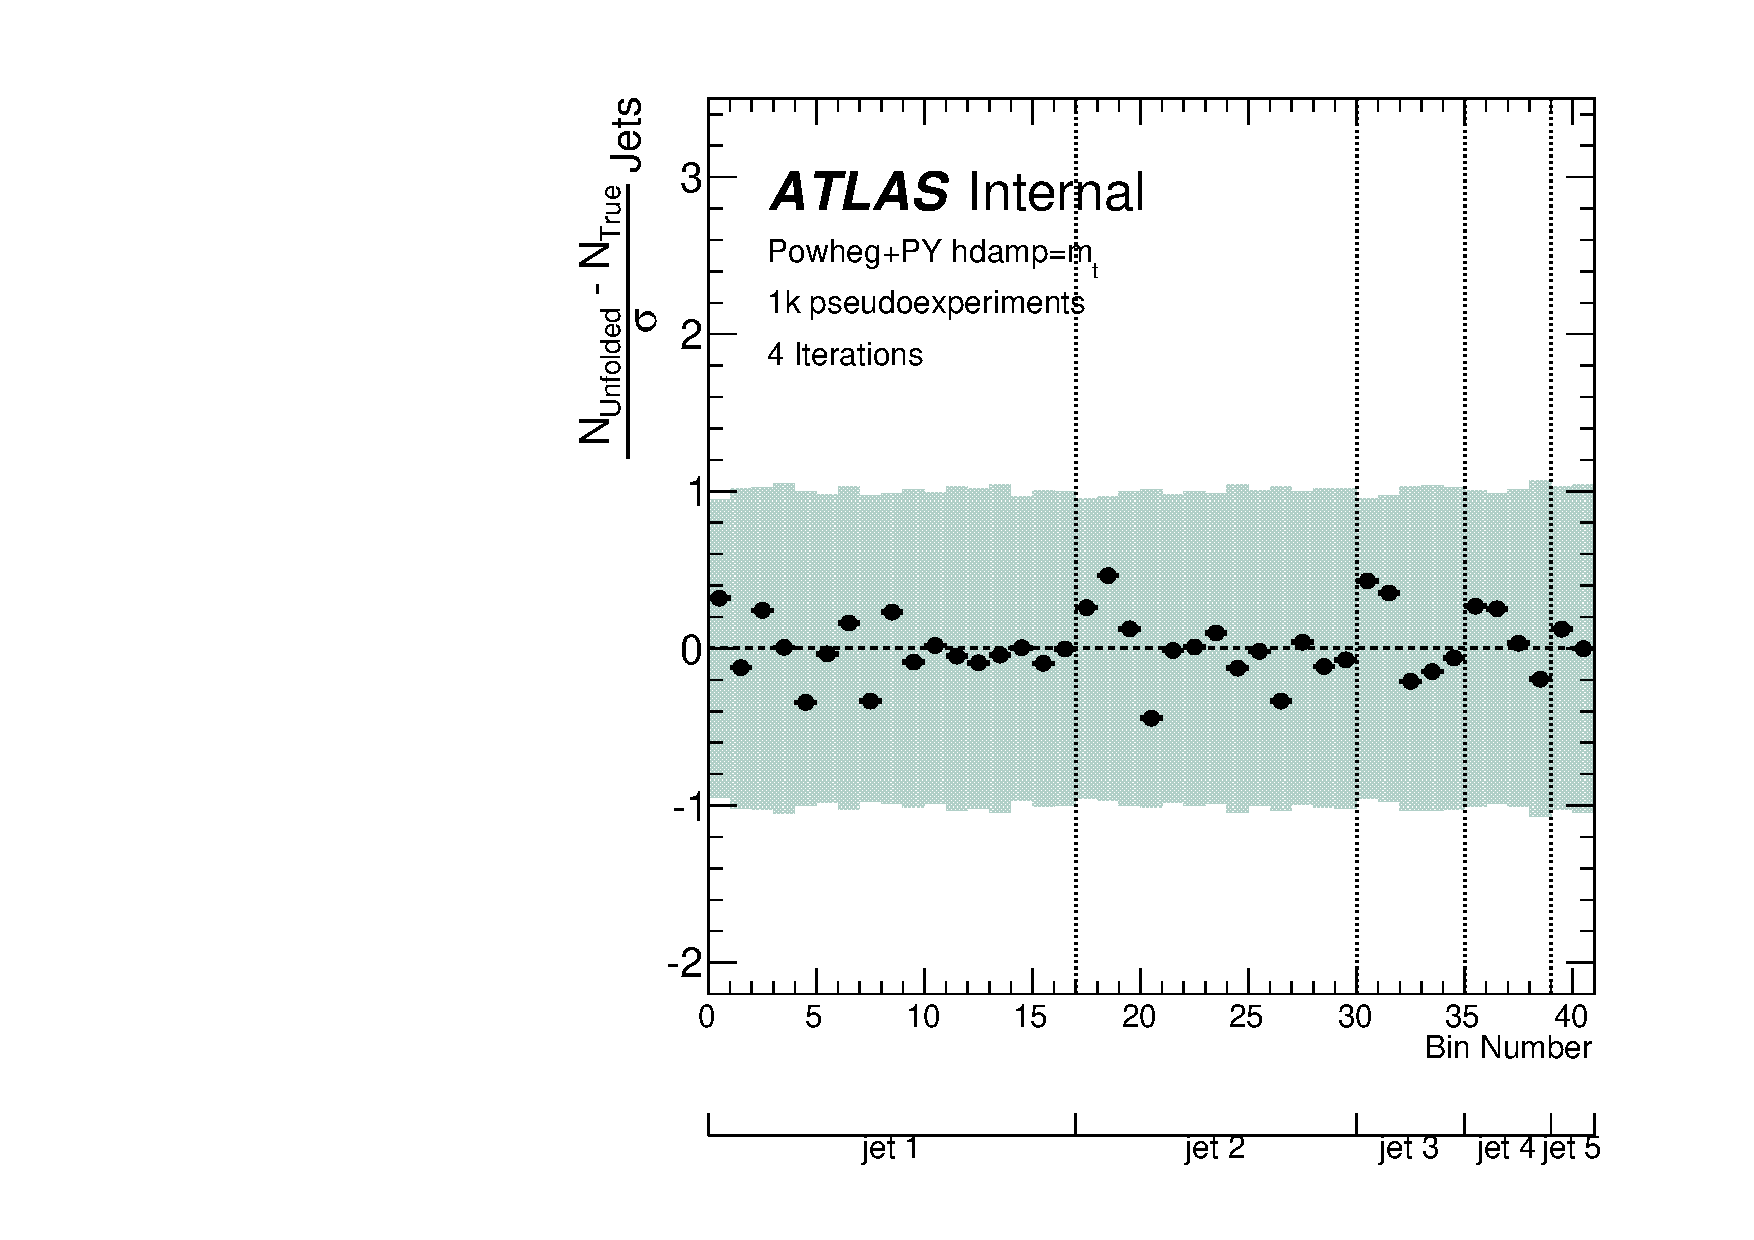
\includegraphics[width=\textwidth]{fig/Stress/110404atlfast/Pull4Iterations.pdf}
\end{subfigure}
\caption{Pull distribution for pseudoexperiments constructed from \newline \hdamp~ simulation unfolded against a matrix filled with the baseline simulation. One thousand pseudoexperiments, each the size of the events in data, are selected from the sample and unfolded. The Bayesian unfolding method with various numbers of iterations is used. Each bin of the distribution over the pseudoexperiments is fit with a gaussian. The black points show the fitted mean of each bin and the blue band shows the fitted sigma.}
\label{fig:hdamppull}
\end{figure}

\clearpage
%\section{Pull \peight}
\begin{figure}
\begin{subfigure}[]{0.5\textwidth}
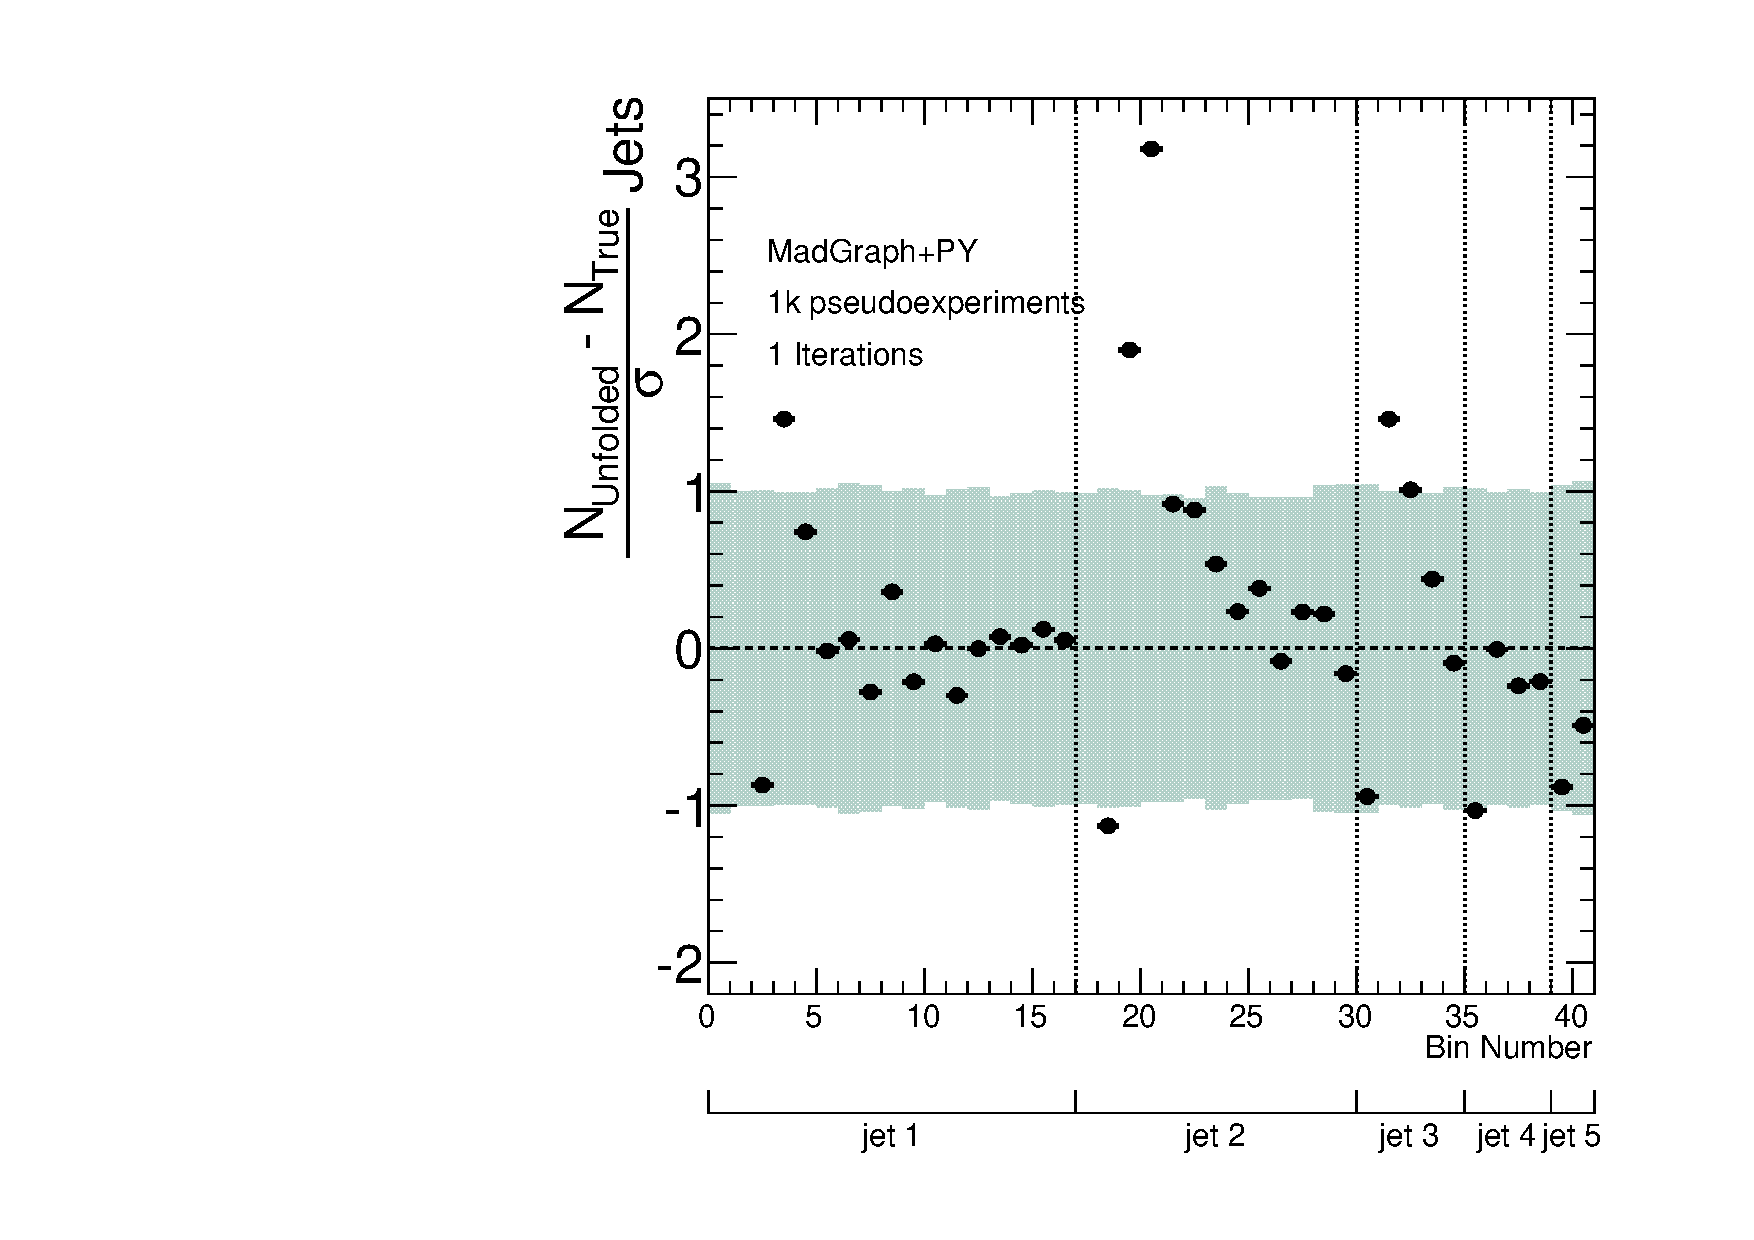
\includegraphics[width=\textwidth]{fig/Stress/110872atlfast/Pull1Iterations.pdf}
\end{subfigure}
~
\begin{subfigure}[]{0.5\textwidth}
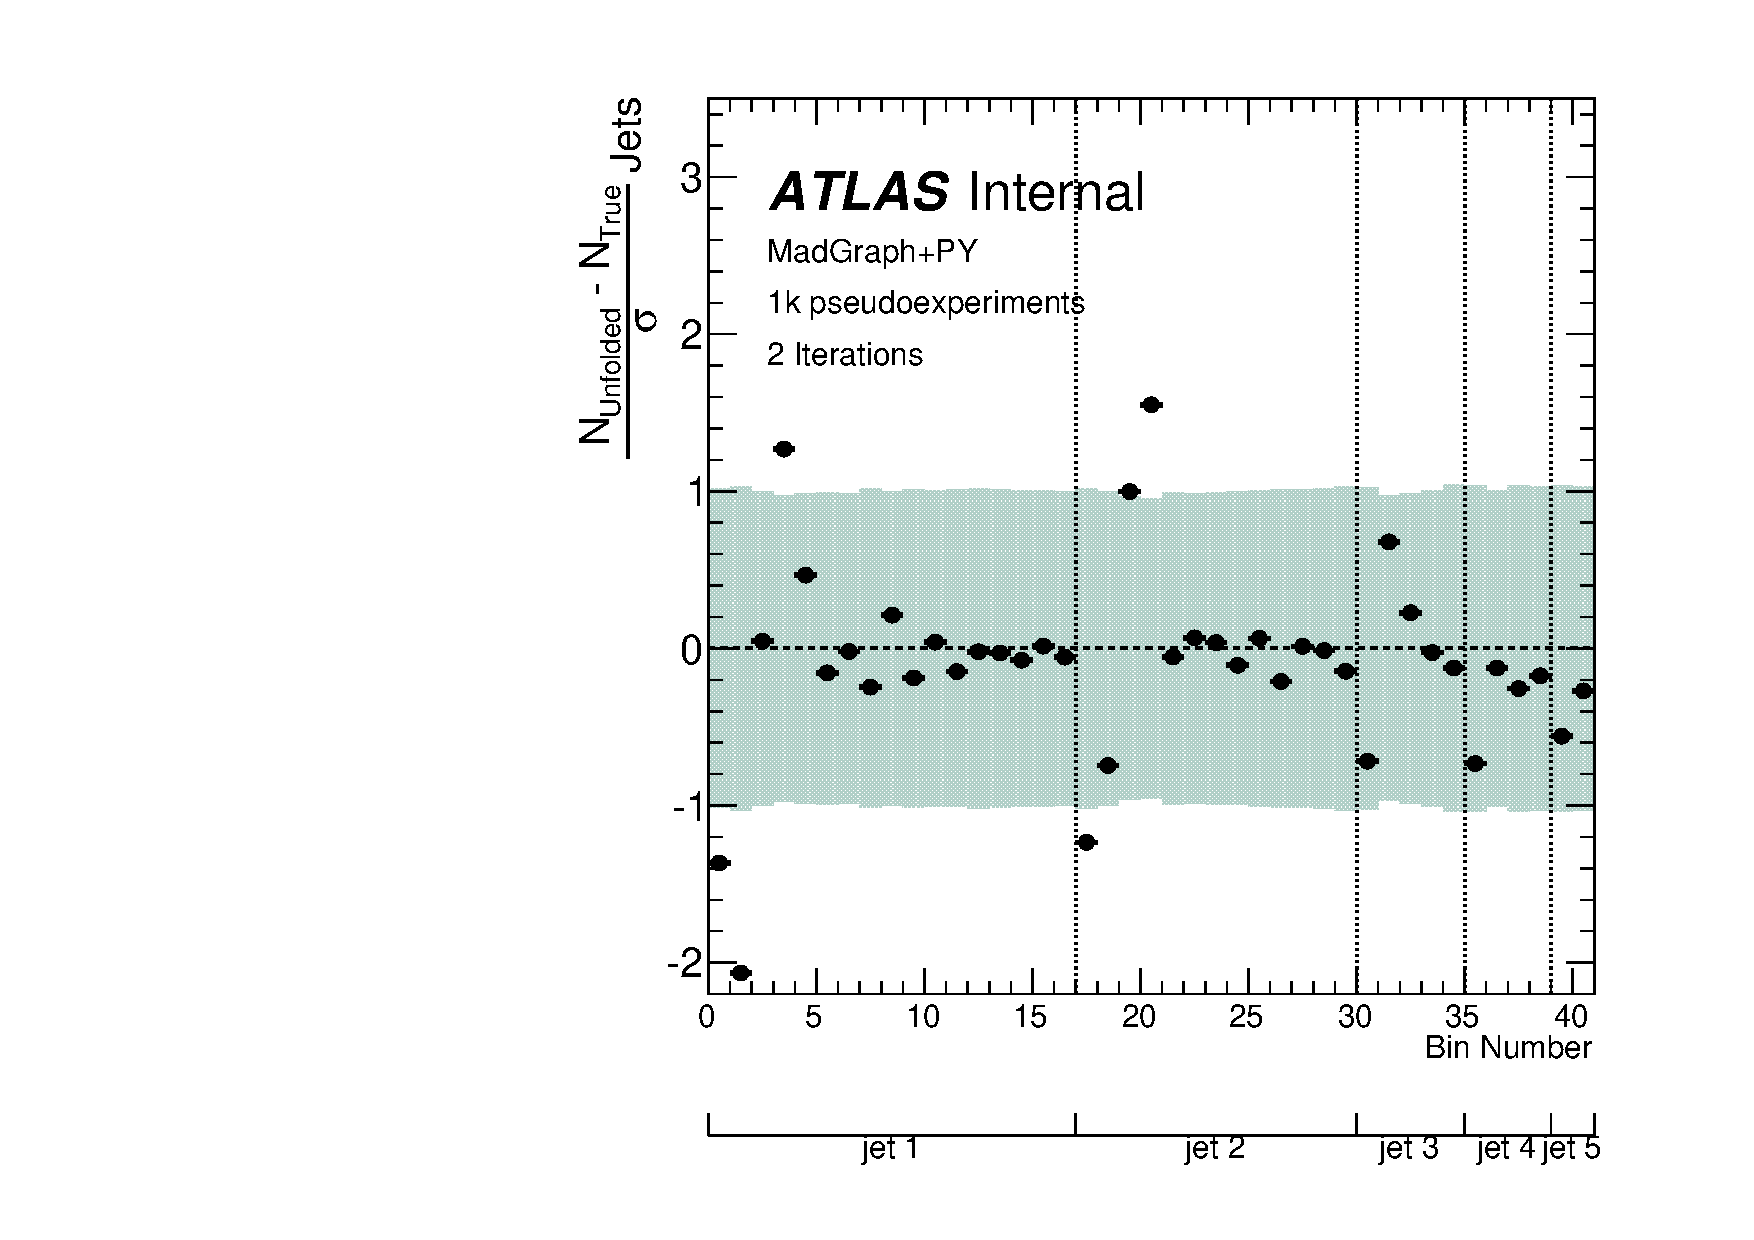
\includegraphics[width=\textwidth]{fig/Stress/110872atlfast/Pull2Iterations.pdf}
\end{subfigure}
\\
\begin{subfigure}[]{0.5\textwidth}
\includegraphics[width=\textwidth]{fig/Stress/110872atlfast/Pull3Iterations.pdf}
\end{subfigure}
~
\begin{subfigure}[]{0.5\textwidth}
\includegraphics[width=\textwidth]{fig/Stress/110872atlfast/Pull4Iterations.pdf}
\end{subfigure}
\caption{Pull distribution for pseudoexperiments constructed from \newline \peight~ simulation unfolded against a matrix filled with the baseline simulation. One thousand pseudoexperiments, each the size of the events in data, are selected from the sample and unfolded. The Bayesian unfolding method with various numbers of iterations is used. Each bin of the distribution over the pseudoexperiments is fit with a gaussian. The black points show the fitted mean of each bin and the blue band shows the fitted sigma.}
\label{fig:p8pull}
\end{figure}
\clearpage
%\section{Pull \powpy\ fullsim}
\begin{figure}
\begin{subfigure}[]{0.5\textwidth}
\includegraphics[width=\textwidth]{fig/Stress/117050fullsim/Pull1Iterations.pdf}
\end{subfigure}
~
\begin{subfigure}[]{0.5\textwidth}
\includegraphics[width=\textwidth]{fig/Stress/117050fullsim/Pull2Iterations.pdf}
\end{subfigure}
\\
\begin{subfigure}[]{0.5\textwidth}
\includegraphics[width=\textwidth]{fig/Stress/117050fullsim/Pull3Iterations.pdf}
\end{subfigure}
~
\begin{subfigure}[]{0.5\textwidth}
\includegraphics[width=\textwidth]{fig/Stress/117050fullsim/Pull4Iterations.pdf}
\end{subfigure}
\caption{Pull distribution for pseudoexperiments constructed from \newline \powpy~ fullsim simulation unfolded against a matrix filled with the baseline simulation. One thousand pseudoexperiments, each the size of the events in data, are selected from the sample and unfolded. The Bayesian unfolding method with various numbers of iterations is used. Each bin of the distribution over the pseudoexperiments is fit with a gaussian. The black points show the fitted mean of each bin and the blue band shows the fitted sigma.}
\label{fig:fspull}
\end{figure}
\clearpage
\begin{figure}
\begin{subfigure}[]{0.5\textwidth}
\includegraphics[width=\textwidth]{fig/Stress/105200atlfast/Pull1Iterations.pdf}
\end{subfigure}
\begin{subfigure}[]{0.5\textwidth}
\includegraphics[width=\textwidth]{fig/Stress/105200atlfast/Pull2Iterations.pdf}
\end{subfigure}
\\
\begin{subfigure}[]{0.5\textwidth}
\includegraphics[width=\textwidth]{fig/Stress/105200atlfast/Pull3Iterations.pdf}
\end{subfigure}
\begin{subfigure}[]{0.5\textwidth}
\includegraphics[width=\textwidth]{fig/Stress/105200atlfast/Pull4Iterations.pdf}
\end{subfigure}
\caption{Bias distribution for pseudoexperiments constructed from \newline \mcnlohw\ simulation unfolded against a matrix filled with the baseline simulation. One thousand pseudoexperiments, each the size of the events in data, are selected from the sample and unfolded. The Bayesian unfolding method with various numbers of iterations is used. Each bin of the distribution over the pseudoexperiments is fit with a gaussian. The black points show the fitted mean of each bin and the blue band shows the fitted sigma.}
\label{fig:mcnlopull}
\end{figure}
\clearpage
\begin{center}
\begin{table}
\begin{tabular}{|l|c|c|c|c|c|c|c|c|}
\hline
Method & 110404 & 117046 & 105860 & 105200 & 110872 & 117050 & 110875 & 110878\\
\hline
Bin-by-bin& -8.0\e{2}& -5.3\e{2}& -5.0\e{2}& -3.8\e{2}& -6.1\e{2}& -2.3\e{2}& -5.4\e{2}& -4.8\e{2}\\ 
1& 1.0& -2.2\e{-1}& 2.2& 4.0& -1.8& 1.2\e{-1}& -1.3& -2.3\\ 
2& 1.2& -8.8\e{-2}& 2.4& 4.4& -1.5& 4.2\e{-2}& -1.3& -2.4\\ 
3& 1.3& -1.1\e{-1}& 2.6& 4.7& -1.4& 4.6\e{-2}& -1.3& -2.4\\ 
4& 1.3& -1.1\e{-1}& 2.5& 4.7& -1.3& 1.2\e{-1}& -1.3& -2.5\\ 
5& 1.3& -1.1\e{-1}& 2.5& 4.8& -1.3& 1.3\e{-1}& -1.3& -2.5\\ 
6& 1.4& -7.2\e{-2}& 2.7& 5.0& -1.3& 9.8\e{-5}& -1.3& -2.5\\ 
7& 1.4& -7.5\e{-2}& 2.8& 5.1& -1.3& 3.4\e{-3}& -1.3& -2.5\\ 
8& 1.5& -2.0\e{-1}& 2.7& 5.1& -1.2& 1.4\e{-1}& -1.2& -2.7\\ 
9& 1.5& -2.0\e{-1}& 2.8& 5.2& -1.2& 1.5\e{-1}& -1.2& -2.7\\ 
\hline
\end{tabular}
\caption{Comparison of the average bias per bin for stress tests with several different ttbar generators and unfolding methods. All samples are atlfast. For each generator, the measured jets from one thousand pseudoexperiments are unfolded against the baseline \powpy\ atlfast response matrix and compared to the input truth spectrum.}
\label{t:bias}
\end{table}
\end{center}
\clearpage
\begin{center}
\begin{table}
\begin{tabular}{|l|c|c|c|c|c|c|c|c|}
\hline
 Iterations & 110404 & 117046 & 105860 & 105200 & 110872 & 117050 & 110875 & 110878\\
\hline
Bin-by-bin& 4.0\e{6}& 2.6\e{6}& 1.9\e{6}& 1.0\e{6}& 2.6\e{6}& 2.0\e{5}& 2.2\e{6}& 2.4\e{6}\\ 
1& 2.2\e{1}& 2.0\e{1}& 2.3\e{1}& 1.1\e{2}& 2.0\e{2}& 7.1\e{-1}& 1.7\e{2}& 3.2\e{2}\\ 
2& 1.4\e{1}& 9.1& 3.7\e{1}& 9.9\e{1}& 8.7\e{1}& 3.8\e{-1}& 1.5\e{2}& 2.9\e{2}\\ 
3& 1.6\e{1}& 7.0& 4.6\e{1}& 1.3\e{2}& 6.1\e{1}& 4.2\e{-1}& 1.5\e{2}& 2.8\e{2}\\ 
4& 1.7\e{1}& 6.7& 5.1\e{1}& 1.6\e{2}& 5.3\e{1}& 6.0\e{-1}& 1.5\e{2}& 2.8\e{2}\\ 
5& 1.8\e{1}& 6.3& 5.6\e{1}& 1.8\e{2}& 4.8\e{1}& 7.0\e{-1}& 1.4\e{2}& 2.8\e{2}\\ 
6& 2.1\e{1}& 5.6& 6.6\e{1}& 2.0\e{2}& 4.7\e{1}& 1.1& 1.4\e{2}& 2.7\e{2}\\ 
7& 2.2\e{1}& 5.5& 7.0\e{1}& 2.2\e{2}& 4.6\e{1}& 1.2& 1.4\e{2}& 2.6\e{2}\\ 
8& 2.2\e{1}& 5.4& 6.7\e{1}& 2.4\e{2}& 3.8\e{1}& 1.4& 1.4\e{2}& 2.7\e{2}\\ 
9& 2.3\e{1}& 5.3& 7.1\e{1}& 2.5\e{2}& 3.7\e{1}& 1.6& 1.4\e{2}& 2.7\e{2}\\ 
\hline
\end{tabular}
\caption{Comparison of the average bias squared per bin for stress tests with several different ttbar generators and unfolding methods. All samples are atlfast. For each generator, the measured jets from one thousand pseudoexperiments are unfolded against the baseline \powpy\ atlfast response matrix and compared to the input truth spectrum.}
\label{t:biassq}
\end{table}
\end{center}
\clearpage
\begin{center}
\begin{table}
\begin{tabular}{|l|c|c|c|c|c|c|c|c|}
\hline
 Method &110404 & 117046 & 105860 & 105200 & 110872 & 117050 & 110875 & 110878\\
\hline
1& 8.1  & 8.5  & 8.7  & 8.0  & 8.1  & 8.6  & 7.6  & 8.7  \\ 
2& 1.1\e{1}  & 1.2\e{1}  & 1.2\e{1}  & 1.1\e{1}  & 1.1\e{1}  & 1.2\e{1}  & 1.1\e{1}  & 1.2\e{1}  \\ 
3& 1.4\e{1}  & 1.4\e{1}  & 1.5\e{1}  & 1.3\e{1}  & 1.4\e{1}  & 1.5\e{1}  & 1.3\e{1}  & 1.5\e{1}  \\ 
4& 1.5\e{1}  & 1.6\e{1}  & 1.7\e{1}  & 1.5\e{1}  & 1.5\e{1}  & 1.6\e{1}  & 1.4\e{1}  & 1.7\e{1}  \\ 
5& 1.7\e{1}  & 1.8\e{1}  & 1.8\e{1}  & 1.6\e{1}  & 1.7\e{1}  & 1.8\e{1}  & 1.6\e{1}  & 1.8\e{1}  \\ 
6& 1.8\e{1}  & 1.9\e{1}  & 2.0\e{1}  & 1.8\e{1}  & 1.8\e{1}  & 1.9\e{1}  & 1.7\e{1}  & 2.0\e{1}  \\ 
7& 1.9\e{1}  & 2.0\e{1}  & 2.1\e{1}  & 1.9\e{1}  & 1.9\e{1}  & 2.0\e{1}  & 1.8\e{1}  & 2.1\e{1}  \\ 
8& 2.0\e{1}  & 2.1\e{1}  & 2.2\e{1}  & 2.0\e{1}  & 2.0\e{1}  & 2.1\e{1}  & 1.9\e{1}  & 2.2\e{1}  \\ 
9& 2.1\e{1}  & 2.2\e{1}  & 2.3\e{1}  & 2.1\e{1}  & 2.1\e{1}  & 2.2\e{1}  & 2.0\e{1}  & 2.3\e{1}  \\ 
\hline
\end{tabular}
\caption{Comparison of the average returned bin error for stress tests with several different ttbar generators and unfolding methods. All samples are atlfast. For each generator, the measured jets from one thousand pseudoexperiments are unfolded against the baseline \powpy\ atlfast response matrix and compared to the input truth spectrum.}
\label{t:err}
\end{table}
\end{center}
\clearpage
\begin{center}
\begin{table}
\begin{tabular}{|l|c|c|c|c|c|c|c|c|}
\hline
 Method & 110404 & 117046 & 105860 & 105200 & 110872 & 117050 & 110875 & 110878\\
\hline
1& 162.20 & 348.55 & 463.69 & 241.11 & 440.84 & 67.66 & 502.50 & 476.26 \\ 
2& 72.40 & 118.68 & 156.97 & 97.56 & 147.88 & 48.41 & 484.10 & 179.55 \\ 
3& 56.05 & 76.47 & 94.68 & 75.87 & 90.89 & 44.91 & 306.33 & 113.96 \\ 
4& 49.86 & 61.21 & 72.91 & 68.48 & 71.84 & 43.44 & 199.33 & 91.37 \\ 
5& 47.48 & 54.45 & 63.00 & 66.06 & 62.27 & 42.96 & 148.26 & 80.78 \\ 
6& 46.70 & 51.33 & 58.18 & 65.62 & 56.25 & 42.83 & 119.98 & 74.81 \\ 
7& 46.00 & 49.18 & 54.97 & 65.24 & 53.14 & 42.71 & 103.28 & 71.36 \\ 
8& 45.49 & 48.04 & 52.77 & 66.20 & 51.17 & 42.76 & 92.02 & 69.23 \\ 
9& 45.23 & 47.12 & 51.38 & 66.55 & 49.81 & 42.75 & 84.55 & 67.70 \\ 
\hline
\end{tabular}
\caption{The \chisq\ of extra jets from the each \ttbar simulation unfolded against a matrix filled with the same baseline \ttbar simulation (\powpy). All samples are atlfast. The same 3\% contribution from Wt is included in both the migration matrix and the unfolding. The Bayesian unfolding method is used with iterations ranging from 1 to 10. One thousand pseudoexperiments, each the size of the events in data, are randomly selected from the sample and unfolded. The \chisq is calculated according to Equation~\ref{eq:unfchi2}. 
The \chisq\ in compares the fully corrected reco jets to truth jets in truth events.}
\end{table}
\label{t:stresschi}
\end{center}
\clearpage
\begin{figure}
\begin{subfigure}[]{0.45\textwidth}
\includegraphics[width=\textwidth]{fig/Stress/105860atlfast/AvgChi2.pdf}
\end{subfigure}
~
\begin{subfigure}[]{0.45\textwidth}
\includegraphics[width=\textwidth]{fig/Stress/110872atlfast/AvgChi2.pdf}
\end{subfigure}
\\
\begin{subfigure}[]{0.45\textwidth}
\includegraphics[width=\textwidth]{fig/Stress/110404atlfast/AvgChi2.pdf}
\end{subfigure}
~
\begin{subfigure}[]{0.45\textwidth}
\includegraphics[width=\textwidth]{fig/Stress/105200atlfast/AvgChi2.pdf}
\end{subfigure}
~
\caption{The \chisq\ of extra jets from the each \ttbar simulation unfolded against a matrix filled with the same baseline \ttbar simulation (\powpy). All samples are atlfast. The same 3\% contribution from Wt is included in both the migration matrix and the unfolding. The Bayesian unfolding method is used with iterations ranging from 1 to 10. One thousand pseudoexperiments, each the size of the events in data, are randomly selected from the sample and unfolded. The \chisq is calculated according to Equation~\ref{eq:unfchi2}. 
The \chisq\ in compares the fully corrected reco jets to truth jets in truth events.}
\end{figure}
\label{f:stresschi}
\clearpage